\documentclass[12pt]{article}

\usepackage[a4paper,inner=1.5in,outer=1in,top=1in,bottom=1in]{geometry}

\usepackage{xcolor}
\usepackage{mathtools}
\DeclareMathOperator{\sech}{sech}

\usepackage{amsmath, amssymb}
\usepackage{algpseudocode}
\usepackage{caption}
\usepackage[most]{tcolorbox}

\newtcolorbox{numvaluesbox}{
    colback=blue!8,
    colframe=blue!45!black,
    boxrule=0.6pt,
    arc=2.5mm,
    left=1.5mm,
    right=1.5mm,
    top=1mm,
    bottom=1mm,
    title={Summary of numerical values},
    fonttitle=\bfseries
}

\newtcolorbox{terminationbox}{
    colback=blue!6,
    colframe=blue!50!black,
    boxrule=0.6pt,
    arc=2.5mm,
    left=1.5mm,
    right=1.5mm,
    top=1mm,
    bottom=1mm,
    title={Termination criteria},
    fonttitle=\bfseries
}

\begin{document}
% % Title page setup
% \title{Research Lab Course Report: Thermodynamics and dynamics of ternary phase separation}
% \author{Malcolm Steen}
% \date{\today}
% \maketitle
% \tableofcontents
% \clearpage  
\tableofcontents
\newpage


\section{Introduction}
There has been theoretical work on ternary systems \cite{Demarchi2023EnzymeEnriched}
There has been work on reconstructing the binodal from an interaction matrix including genetic models \cite{Milani2007,WEI200691} analytical approaches \cite{WEI200691} and convexification of the energy landscape \cite{Mao2019}
Phase separation in multicomponent fluids provides a general physical framework for understanding how a homogeneous mixture can spontaneously demix into coexisting phases with distinct compositions. At its core, this phenomenon emerges from the competition between entropy, which favors mixing and intermolecular interactions, which can favor segregation. In biological and soft-matter systems, this balance underlies liquid-liquid phase separation and the formation of condensed phases with well-defined interfaces and characteristic dynamical behavior. A theoretical description of such systems therefore requires linking equilibrium thermodynamics, interfacial physics and diffusive transport within a unified framework.


\section{Liquid-liquid phase separation}
In this chapter, we develop the theoretical basis for the ternary phase-separating system studied in this thesis. We begin with the thermodynamics of incompressible mixtures and derive the conditions for local and global stability, which define the spinodal, binodal and critical point. We then introduce a mean-field lattice description that leads to a Flory-Huggins free-energy functional with gradient terms, allowing spatially heterogeneous states and diffuse interfaces to be described on a continuum level. Building on this free-energy framework, we formulate the diffusive dynamics of phase separation in terms of coupled Cahn-Hilliard equations for the conserved volume fractions. We further discuss the thermodynamic definition of surface tension in ternary systems and, finally, outline the numerical methods used to compute equilibrium profiles and interfacial properties. Together, these results establish the theoretical framework that will be used throughout the remainder of this thesis to analyze phase behavior, interface formation and relaxation dynamics in ternary mixtures.
\subsection{Thermodynamics of a ternary mixture}\label{ss:thermodynamics}
We begin by considering the a complex mixture of three components at constant temperature \(T\), Volume \(V\) and particle numbers \(N_0, N_1, N_2\). This system is best described by the Helmholtz free-energy,
\(F=U-TS\).
For simplicity, we only consider an incompressible fluid with constant volume and molecular volume \(\nu\).
We also enforce the null-void condition meaning that vacancies caused by removing one particle must be filled by another particle.
Under these conditions we can introduce the relationship
\begin{equation}
    \phi_0 + \phi_1 + \phi_2 = 1
    \label{eq:incompressibility}
\end{equation}
where \(\phi_i = \frac{N_i \nu}{V}\) is the volume fraction of component \(i\). This relationship allows us to reduce the number of independent variables from three to two.
Thus the free-energy can be written as \(F(\phi_1, \phi_2)\).


\subsubsection{Local stability analysis}
In a homogeneous system the total free-energy is equal to \(F = V f(\phi_1, \phi_2)\), where \(f(\phi_1,\phi_2)\) is the free-energy density. The local stability of this system is determined by the curvature of \(f(\phi_1,\phi_2)\).
To make this precise we consider small spatial fluctuations \(\delta \phi_1(\mathbf{r})\) and \(\delta \phi_2(\mathbf{r})\) around a homogeneous state \((\phi_1,\phi_2)\). Since the total number of particles is conserved, these fluctuations satisfy
\[
    \int_V \delta \phi_i(\mathbf{r})\, d\mathbf{r} = 0, \qquad i \in \{1,2\}.
\]
Expanding the free-energy density to second order yields
\[
    f(\phi_1 + \delta \phi_1, \phi_2 + \delta \phi_2)
    = f(\phi_1,\phi_2)
    + \sum_{i=1}^2 \frac{\partial f}{\partial \phi_i} \delta \phi_i
    + \frac{1}{2} \sum_{i,j=1}^2 \frac{\partial^2 f}{\partial \phi_i \partial \phi_j} \delta \phi_i \delta \phi_j
    + \mathcal{O}(\delta \phi^3).
\]
After integrating over the volume, the linear term vanishes because the spatial average of each \(\delta \phi_i\) is zero. The corresponding change in free-energy is therefore
\[
    \delta F = \frac{1}{2} \int_V \sum_{i,j=1}^2 H_{ij} \, \delta \phi_i(\mathbf{r}) \, \delta \phi_j(\mathbf{r}) \, d\mathbf{r},
\]
where
\[
    H_{ij} = \frac{\partial^2 f}{\partial \phi_i \partial \phi_j}
\]
is the Hessian matrix of the free-energy density. Local stability requires \(\delta F > 0\) for every nonzero fluctuation, which is equivalent to the Hessian being positive definite.
If one eigenvalue of the Hessian becomes negative, then there exists a fluctuation that lowers the free-energy and the homogeneous state is locally unstable towards phase separation.
The set of points where one or both eigenvalues vanish defines the spinodal. For a system with two independent variables the spinodal is given by the condition
\[
    \det H = 0.
\]
Since the spinodal is given by a single condition, it generally forms one or more curves in the \((\phi_1, \phi_2)\) plane separating locally stable from locally unstable regions.


\subsubsection{Global stability analysis}
Local stability does not imply global stability. Although a homogeneous system does not spontaneously phase separate, there might still exist a phase separated state with lower free-energy. To determine whether such a state exists we examine the free-energy of a two-phase state.
Again neglecting the interfacial energy, the free-energy of a two-phase system is given by
\begin{equation}
    F = V_1 f(\phi_1^{(1)},\phi_2^{(1)}) + V_2 f(\phi_1^{(2)},\phi_2^{(2)})
    \label{eq:free_energy_two_phase}
\end{equation}
where \(V_1\) and \(V_2\) are the volumes of phase \(1\) and \(2\), respectively. The total volume and the total number of particles need to be conserved, which yields the three constraints
\[
    V_1 \phi_i^{(1)} + V_2 \phi_i^{(2)} = V\bar\phi_i, \qquad i \in \{1,2\},
\]
and
\[
     V_1 + V_2 = V,
\]
where \(\bar\phi_i\) is the mean volume fraction of species \(i\). Therefore the six variables reduce to three independent variables, which can be chosen as \(\phi_1^{(1)}, \phi_2^{(1)}, V_1\).
Minimizing the free-energy in Eq.~\ref{eq:free_energy_two_phase} with respect to these three variables yields the coexistence conditions
\begin{equation}
    \begin{aligned}
        \frac{\partial f}{\partial \phi_1}(\phi_1^{(1)},\phi_2^{(1)}) &= \frac{\partial f}{\partial \phi_1}(\phi_1^{(2)},\phi_2^{(2)}) \\
        \frac{\partial f}{\partial \phi_2}(\phi_1^{(1)},\phi_2^{(1)}) &= \frac{\partial f}{\partial \phi_2}(\phi_1^{(2)},\phi_2^{(2)}) \\
        \sum_{i=1}^2 \phi_i^{(1)} \frac{\partial f}{\partial \phi_i}(\phi_1^{(1)},\phi_2^{(1)}) - f(\phi_1^{(1)},\phi_2^{(1)}) &= \sum_{i=1}^2 \phi_i^{(2)} \frac{\partial f}{\partial \phi_i}(\phi_1^{(2)},\phi_2^{(2)}) - f(\phi_1^{(2)},\phi_2^{(2)})
    \end{aligned}
    \label{eq:coexistence_conditions_derivation}
\end{equation}

Identifying the exchange chemical potentials  and the osmotic pressure
\begin{subequations}
    \begin{align}
        \mu_i &= \frac{\partial f}{\partial \phi_i}, \\
    \Pi &= \sum_{i=1}^2 \phi_i \frac{\partial f}{\partial \phi_i} - f,
    \end{align}
    \label{eq:chemical_potential_and_pressure_definitions}
\end{subequations}
we see that at coexistence the chemical potentials and osmotic pressure of both phases need to be equal.
\begin{subequations}
    \begin{align}
        \mu_1(\phi_1^{(1)},\phi_2^{(1)}) &= \mu_1(\phi_1^{(2)},\phi_2^{(2)}) \\
        \mu_2(\phi_1^{(1)},\phi_2^{(1)}) &= \mu_2(\phi_1^{(2)},\phi_2^{(2)}) \\
        \Pi(\phi_1^{(1)},\phi_2^{(1)}) &= \Pi(\phi_1^{(2)},\phi_2^{(2)})
    \end{align}
    \label{eq:coexistence_conditions}
\end{subequations}
The pairs of compositions that satisfy these conditions define the coexistence points and the set of all such points forms the binodal in the \((\phi_1, \phi_2)\) plane.\\

\begin{minipage}{0.95\textwidth}
    \centering
    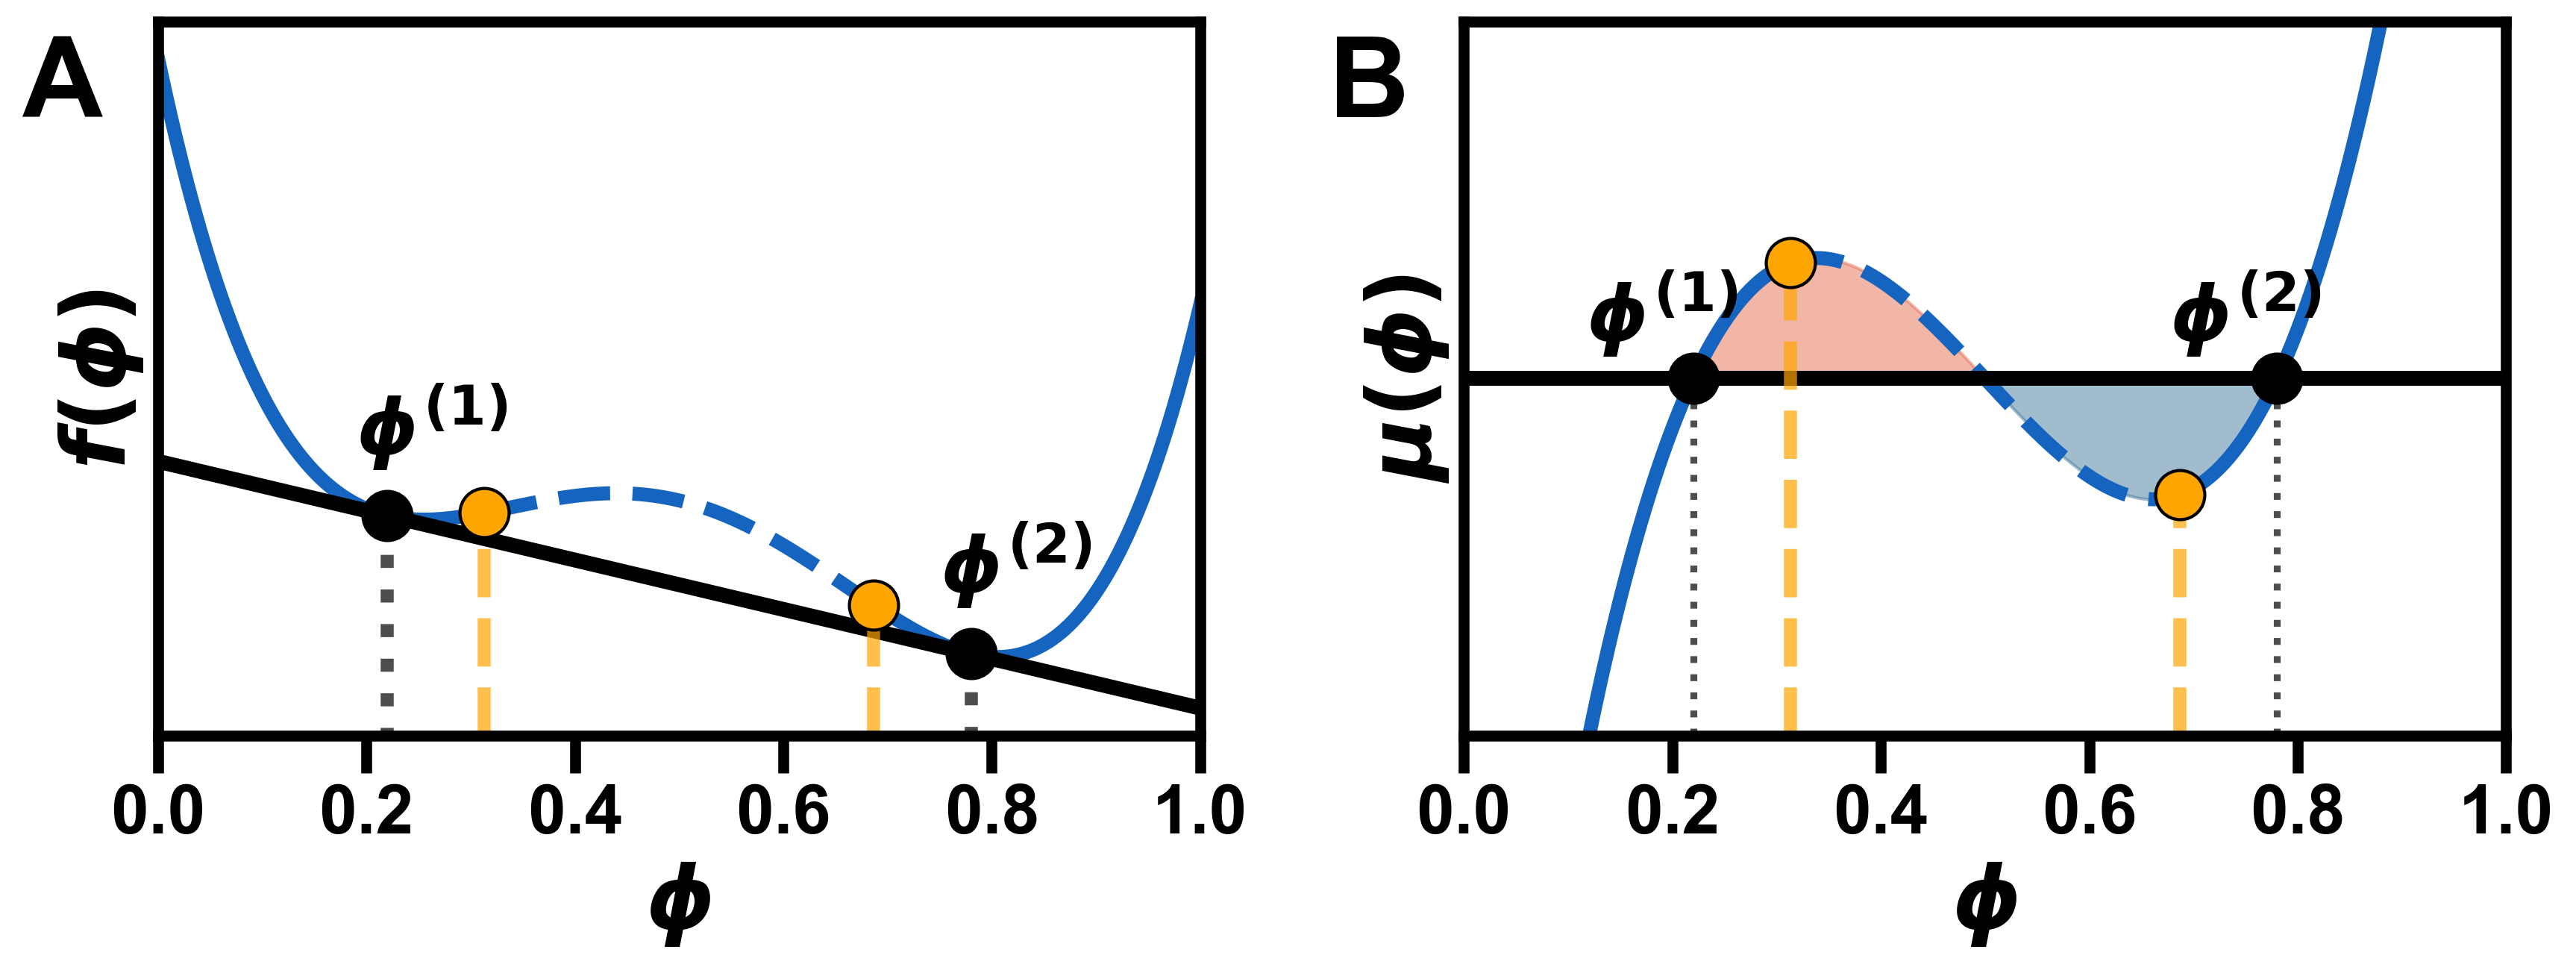
\includegraphics[width=0.98\textwidth]{figures/common_tangent.png}
    \captionof{figure}{Maxwell construction for a binary mixture. (A) The free-energy $f(\phi)$ (blue) and the common tangent (black) at the coexisting compositions $\phi^{(1)}$ and $\phi^{(2)}$. The spinodal points (orange) mark the limits of local stability. (B) The chemical potential $\mu(\phi)$ and the tangent slope (black). The blue and red areas between $\mu(\phi)$ and the tangent slope are equal at coexistence, reflecting the equal pressure requirement. Note that for the ternary system the geometric objects are more complicated, but the same principles apply.}
    \label{fig:common_tangent}
\end{minipage}\\

Geometrically, these conditions correspond to a Maxwell construction for the free-energy surface \(f(\phi_1, \phi_2)\). The slopes of the coexistence points are the same corresponding to equal chemical potentials (see Fig.~\ref{fig:common_tangent}A). The equal area condition in the Maxwell construction reflects the equal pressure requirement at coexistence (see Fig.~\ref{fig:common_tangent}B).\\


In general the spinodal lies inside the binodal, since local instability implies global instability.\\
\begin{minipage}{0.45\textwidth}
    The converse is not true: a system can be locally stable but globally unstable. The region between the binodal and spinodal is called the metastable region.
    In the metastable region phase separation is thermodynamically favorable, but it requires crossing a finite free-energy barrier, so demixing proceeds through nucleation of a droplet.
    Inside the spinodal this barrier disappears and the homogeneous phase becomes unstable with respect to infinitesimal fluctuations, leading instead to spontaneous spinodal decomposition
    (see Fig.~\ref{fig:metastable}).
\end{minipage}%
\hfill
\begin{minipage}{0.5\textwidth}
    \centering
    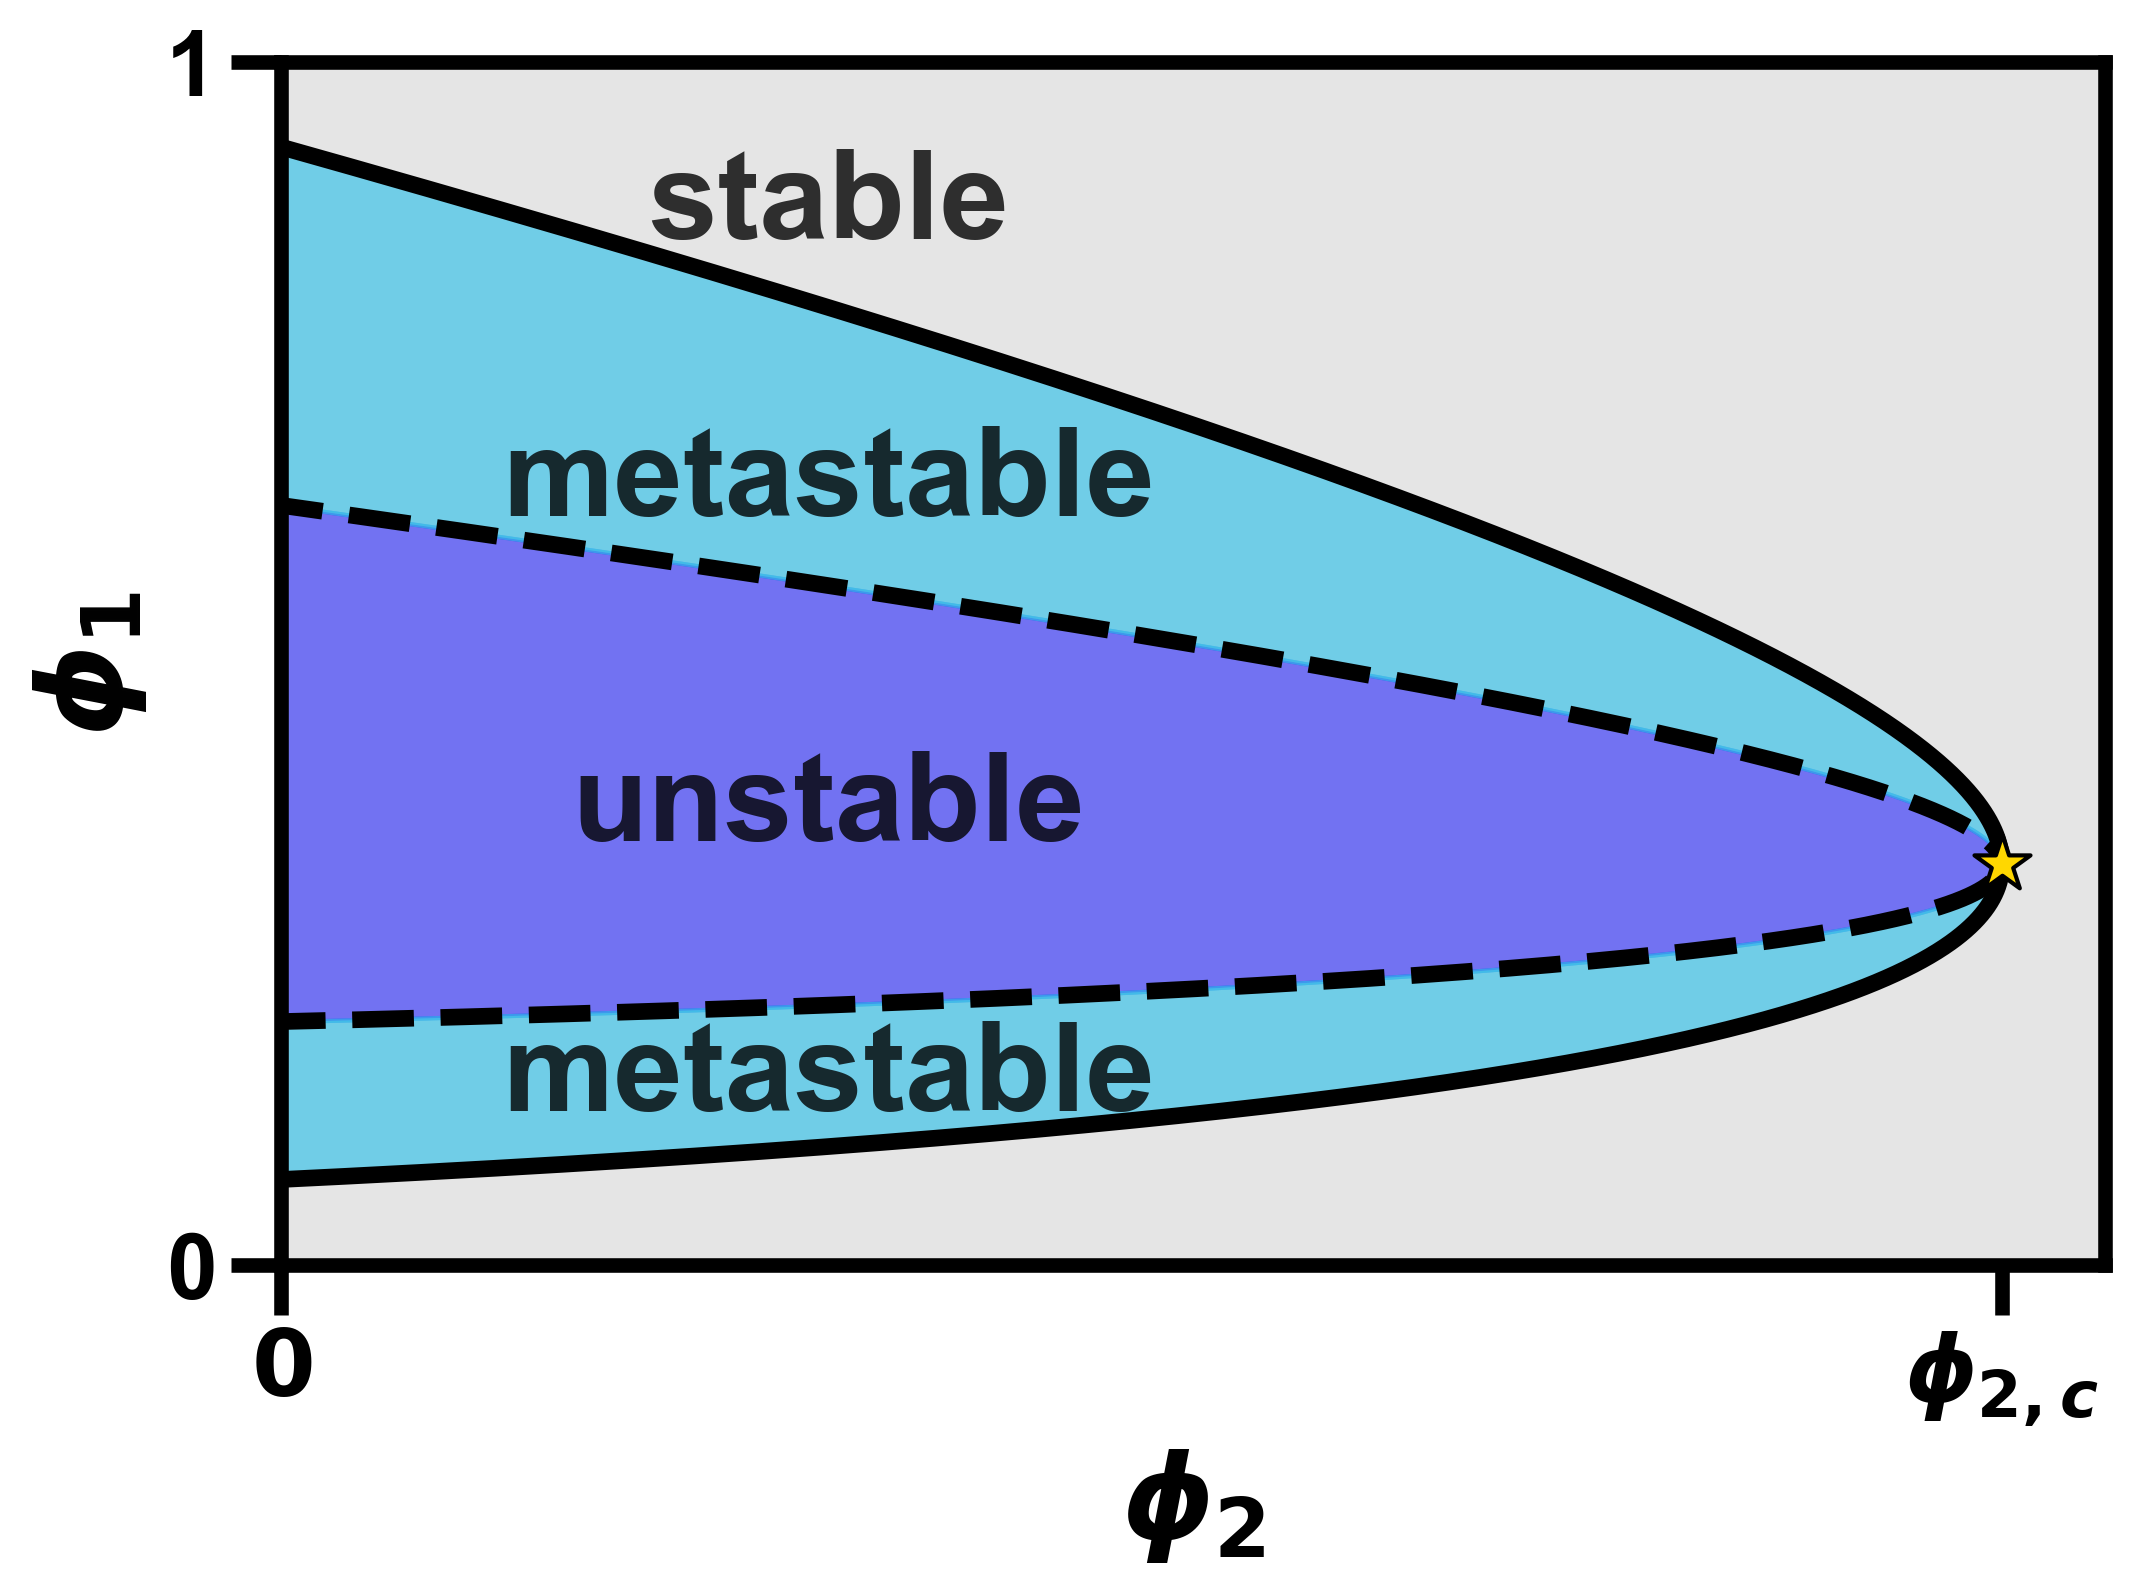
\includegraphics[width=0.98\textwidth]{figures/metastable.png}
    \captionof{figure}{Phase diagram of ternary system showing the binodal (solid black line), spinodal (dashed black line),
    and the regions of stability, metastability and instability of the homogenous state as well as the critical point (gold star).  }
    \label{fig:metastable}
\end{minipage}\\


\subsubsection{Critical point}\label{sss:critical_point}

The critical point is the endpoint of the binodal curve at which the two
coexisting phases become identical. At this point the difference between the
two equilibrium compositions vanishes continuously and the tie-line shrinks to
a single point in composition space. Consequently, the binodal and spinodal
curves intersect at the critical point (see Fig.~\ref{fig:metastable}).

Since the critical point lies on the spinodal, the free
energy must satisfy the same stability condition. In particular, the determinant of the Hessian vanishes,
\begin{equation}
\det\!\left(\frac{\partial^2 f}{\partial \phi_i \partial \phi_j}\right)=0.
\end{equation}

Geometrically, the critical point marks the transition between first- and
second-order phase transition behavior along the coexistence curve.
Here it helps to think about different paths in composition space that cross the binodal curve.
Away from the critical point, crossing the binodal leads to a discontinuous
change in the equilibrium composition. The system separates into two-phases
with finite differences in their volume fractions. This discontinuous change
is characteristic of a first-order phase transition.

At the critical point, however, the difference between the coexisting phase
compositions arises continuously. In this sense, the critical point represents
a second-order phase transition in composition space.

 Mathematically, the emergence of two minima from a single minimum in the free
energy occurs precisely when the third derivative of the free-energy vanishes
along the unstable direction. Denoting by $v_i$ the eigenvector corresponding
to the vanishing eigenvalue of the Hessian, this condition can be written as
\begin{equation}
\sum_{i,j,k} v_i v_j v_k
\frac{\partial^3 f}{\partial \phi_i \partial \phi_j \partial \phi_k}=0.
\label{eq:third_derivative}
\end{equation}
The emergence of two minima from a single minimum is illustrated in Fig.~\ref{fig:critical_point_schematic}.\\

\begin{minipage}{0.95\textwidth}
    \centering
    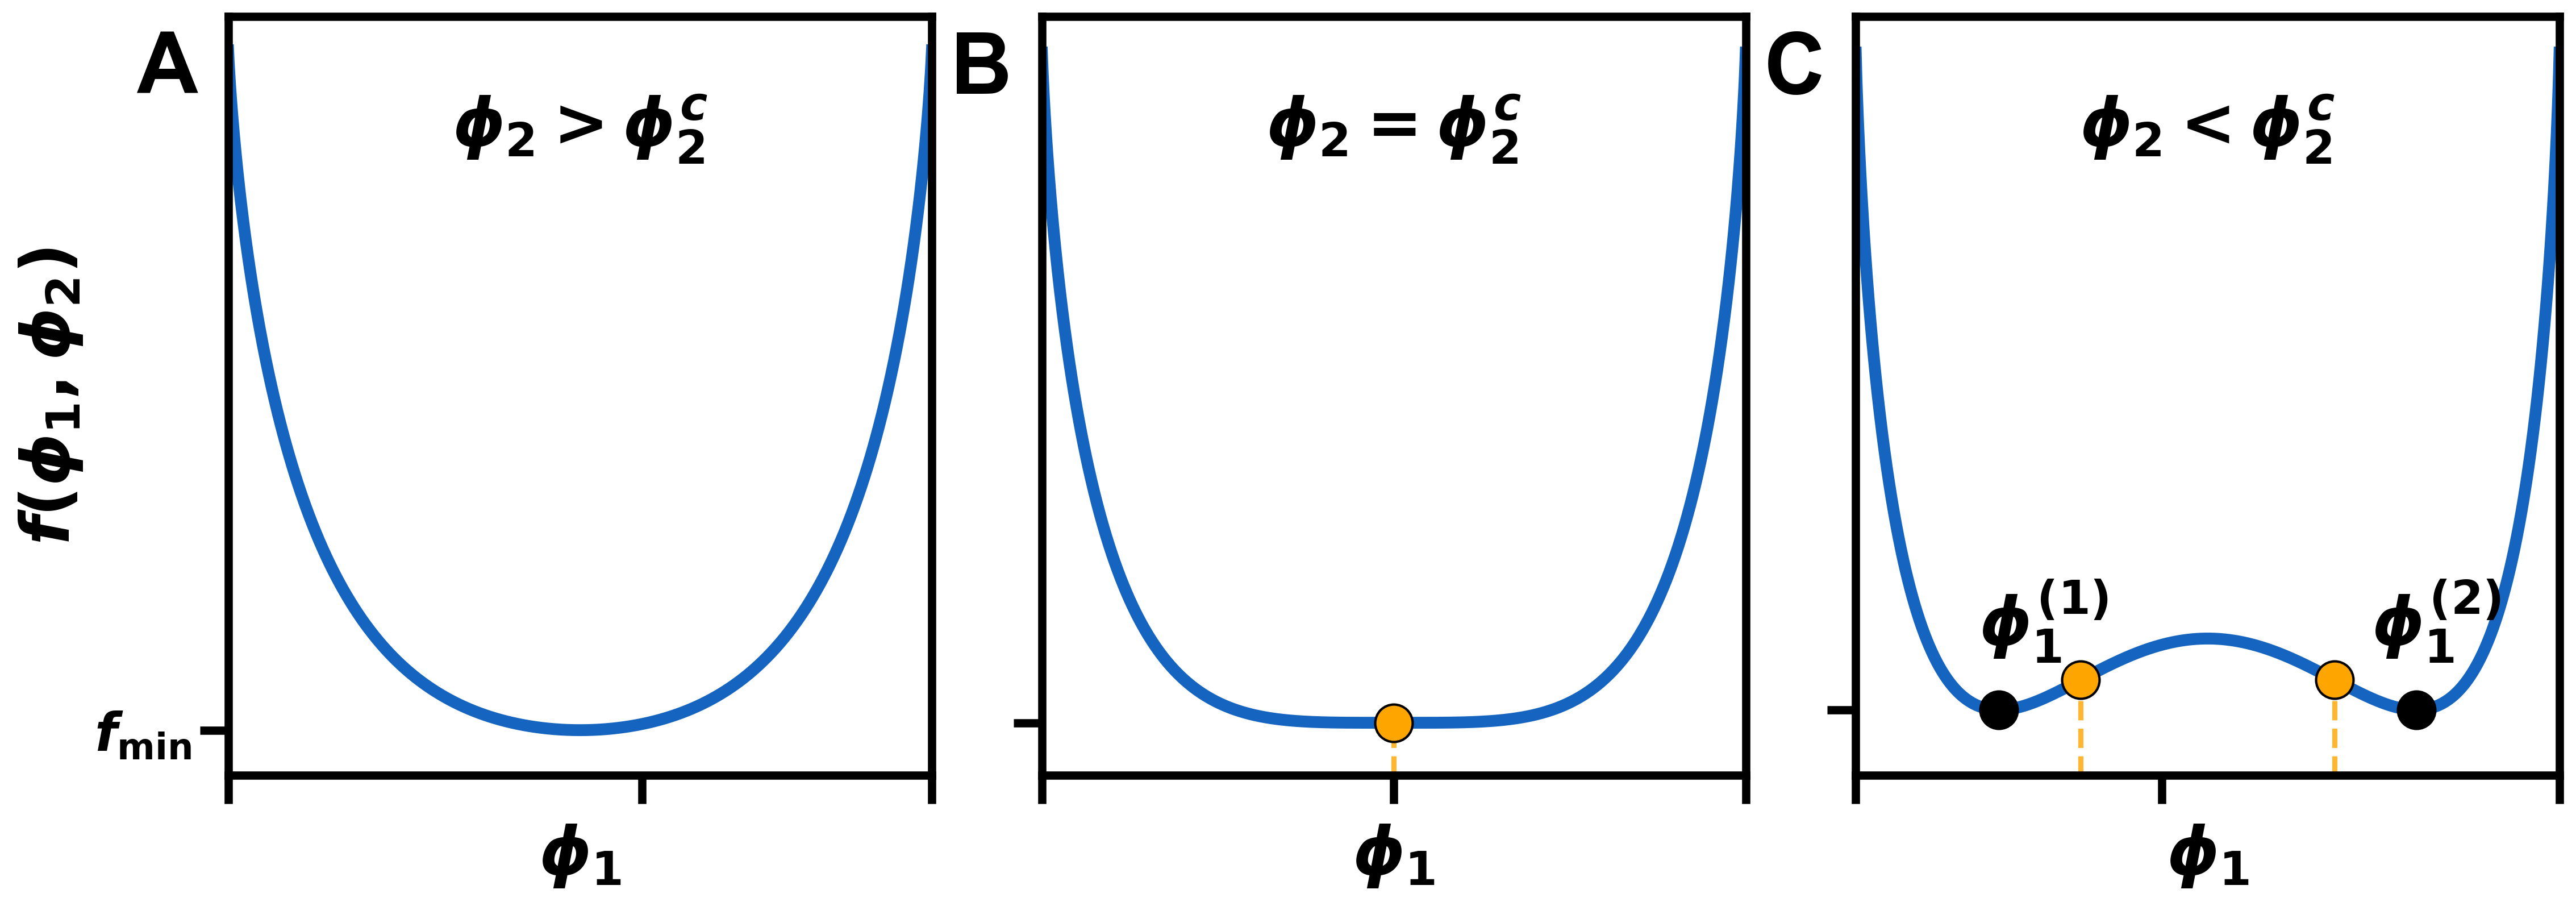
\includegraphics[width=0.98\textwidth]{figures/critical_point_schematic.png}
    \captionof{figure}{5hree cross-sections of the free-energy landscape of the ternary system in Fig.~\ref{fig:metastable}.
    For $\phi_2 > \phi_{2,c}$ (A) the free-energy has a single minimum corresponding to a homogeneous phase.
    For $\phi_2 < \phi_{2,c}$ (C) the free-energy has two minima corresponding to two coexisting phases.
    At the critical point $\phi_2 = \phi_{2,c}$ (B) the two minima merge into a single minimum, marking the onset of phase separation.}
    \label{fig:critical_point_schematic}
\end{minipage}\\

Close to the critical point, the system exhibits scaling behavior that is largely independent of microscopic details.
Within Flory-Huggins theory, this behavior is described by mean-field power laws.

In particular, the difference between the coexisting phase compositions and other
thermodynamic quantities follow power-law relations controlled by universal
critical exponents \cite{Sariban1987FloryHugginsCritical,Binder2005PolymerSolvent}.
These scaling relations will be of interest later on.



\subsection{Mean-field approximation of lattice interactions}
In the previous sections we have discussed properties of the free-energy and how these properties can drive phase separation. In this section we will focus on the exact form of the free-energy.
\subsubsection{Lattice model}
We start by considering a one dimensional lattice model with \(N\) lattice sites and three possible states at each lattice site \(0, 1, 2\) where the total number of each state is conserved.
The lattice sites all have equal lattice spacing \(a\) regardless of their state.
In the null-void case which we are investigating, vacant lattice sites are not allowed and thus the number of independent variables reduces from three to two
\[
\sigma_0 + \sigma_1 + \sigma_2 = 1.
\]
Interactions between lattice sites are restricted to nearest neighbors and have interaction energies \(\tilde{\epsilon}_{ij}\) where \(i,j \in \{1,2\}\).
Note that since we are investigating the reduced system the interaction energies \(\tilde{\epsilon}_{ij}\) have absorbed the interactions with the zeroth component.\\
The full Hamiltonian has the form:
\begin{equation}
\label{eq:ising_hamiltonian}
H = \sum_{n}^{N} \tilde{\epsilon}_{11} \sigma_1^{(n)} \sigma_1^{(n+1)} 
+ \tilde{\epsilon}_{22} \sigma_2^{(n)} \sigma_2^{(n+1)} 
+ \tilde{\epsilon}_{12} \left(\sigma_1^{(n)} \sigma_2^{(n+1)} + \sigma_2^{(n)} \sigma_1^{(n+1)}\right)
\end{equation}
Reducing the number of states introduces linear terms, but because the total number of each state is conserved these terms simply add a constant to the energy and can thus be neglected.

\subsubsection{Mean-field and continuum limit}

We now rewrite the same-species and cross-species nearest-neighbor interactions in a form that separates local and gradient contributions:
\[
\begin{aligned}
    2\sigma_j^n\sigma_j^{n+1}
    &= (\sigma_j^n)^2 + (\sigma_j^{n+1})^2 - (\sigma_j^{n+1}-\sigma_j^n)^2, \\
    \sigma_1^n \sigma_2^{n+1} + \sigma_2^n \sigma_1^{n+1}
    &= \sigma_1^n \sigma_2^n + \sigma_1^{n+1}\sigma_2^{n+1}
    - (\sigma_1^{n+1}-\sigma_1^n)(\sigma_2^{n+1}-\sigma_2^n).
\end{aligned}
\]

We then introduce a mean-field approximation by replacing the occupation variables \(\sigma_i^n\) by their local averages \(\langle \sigma_i^n \rangle\). In a second step, we assume that these local averages vary smoothly on the scale of the lattice spacing \(a\).
we define continuum fields \(\phi_i(x)\) through
\[
\langle \sigma_i^n \rangle \rightarrow \phi_i(x),
\qquad
\langle \sigma_i^{n+1} - \sigma_i^n \rangle \rightarrow a\,\phi_i'(x).
\]
where the prime denotes differentiation with respect to \(x\).

Using the continuum correspondence
\[
\sum_n \rightarrow \frac{1}{a}\int dx,
\]
the interaction energy in Eq.~\ref{eq:ising_hamiltonian} takes the form \textcolor{red}{Perhaps add the full calculations in the appendix?}
\[
E
=
\frac{1}{a}\int dx\,
\left[
\frac{1}{2}\phi_i(x)\tilde{\epsilon}_{ij}\phi_j(x)
-
\frac{a^2}{2}\phi_i'(x)\tilde{\epsilon}_{ij}\phi_j'(x)
\right],
\]
where Einstein summation over repeated indices is implied.

To obtain the entropic contribution, we consider a lattice with \(N\) sites, of which \(N_1\) are occupied by species 1, \(N_2\) by species 2 and \(N-N_1-N_2\) by species 0. The number of distinct arrangements is given by the multinomial coefficient
\[
\Omega = \frac{N!}{(N-N_1-N_2)!N_1!N_2!}.
\]
The entropy \(S = k_B \ln \Omega\) then yields, using Stirling's approximation,
\[
\frac{S}{N}
=
-k_B\left[
(1-\phi_1-\phi_2)\ln(1-\phi_1-\phi_2)
+\phi_1\ln\phi_1
+\phi_2\ln\phi_2
\right],
\]
where \(\phi_i = N_i/N\) are the volume fractions.

The transition from this global expression to a continuum entropy functional is more subtle; for a more detailed discussion, see \cite{Blom2024}. Here we employ a local density approximation and assume that the system can be partitioned into many small coarse-graining cells, each characterized by local volume fractions \(\phi_1(x)\) and \(\phi_2(x)\). The total mixing entropy is then approximated as the sum of the entropies of these cells, which in the continuum limit gives
\[
\begin{aligned}
TS
=
-\frac{k_B T}{a}\int dx\,
\Big[&
\phi_1(x)\ln\phi_1(x)
+\phi_2(x)\ln\phi_2(x)\\
+&(1-\phi_1(x)-\phi_2(x))\ln(1-\phi_1(x)-\phi_2(x))
\Big].\\
\end{aligned}
\]

Combining the energetic and entropic contributions, the free-energy functional \(F=E-TS\) becomes
\begin{equation}
\label{eq:fh_free_energy}
\begin{aligned}
F[\phi_1,\phi_2]
=
\frac{k_B T}{a}\int dx\,
\Big[&
\frac{1}{2}\phi_i\tilde{\chi}_{ij}\phi_j
+
\frac{1}{2}\phi_i'(x)\tilde{\kappa}_{ij}\phi_j'(x)\\
+&
\phi_1\ln\phi_1
+
\phi_2\ln\phi_2
+
(1-\phi_1-\phi_2)\ln(1-\phi_1-\phi_2)
\Big],\\
\end{aligned}
\end{equation}
where, in the present lattice model, we define
\[
\tilde{\chi}_{ij}=\frac{\tilde{\epsilon}_{ij}}{k_B T},
\qquad
\tilde{\kappa}_{ij}=-\frac{a^2}{k_B T}\tilde{\epsilon}_{ij}.
\]

The corresponding free-energy density \(f\) is therefore
\begin{equation}
\label{eq:fh_free_energy_density}
\begin{aligned}
\frac{f(\phi_1,\phi_2)}{k_B T a^{-1}}
=&
\frac{1}{2}\phi_i\tilde{\chi}_{ij}\phi_j
+
\frac{1}{2}\phi_i'(x)\tilde{\kappa}_{ij}\phi_j'(x)\\
+&
\phi_1\ln\phi_1
+
\phi_2\ln\phi_2
+
(1-\phi_1-\phi_2)\ln(1-\phi_1-\phi_2).\\
\end{aligned}
\end{equation}


For the inhomogeneous system, the corresponding exchange chemical potentials and osmotic pressure are

\begin{subequations}
\begin{align}
\frac{\mu_i}{k_B T a^{-1}}
&=
\tilde{\chi}_{ij}\phi_j
+
\ln\phi_i
-
\ln(1-\phi_1-\phi_2)
-
\tilde{\kappa}_{ij}\phi_j'',
\\
\frac{\Pi}{k_B T a^{-1}}
&=
-\ln(1-\phi_1-\phi_2)
+
\frac{1}{2}\phi_i\tilde{\chi}_{ij}\phi_j
-
\phi_i\tilde{\kappa}_{ij}\phi_j''
+
\frac{1}{2}\phi_i'\tilde{\kappa}_{ij}\phi_j'.
\end{align}
\label{eq:chemical_potential_and_pressure}
\end{subequations}


In this derivation, the reduced Flory-Huggins interaction parameters and the reduced gradient coefficients are both determined by the microscopic interaction matrix \(\tilde{\epsilon}_{ij}\) and are therefore not independent. It should be emphasized, however, that alternative derivations of Flory-Huggins free energies can lead to different relations between \(\tilde{\chi}_{ij}\) and \(\tilde{\kappa}_{ij}\) and the gradient coefficients may even depend on the local volume fractions \cite{Tang1991FreeEnergyFunctional,Lifschitz1993InterfacialBehavior}. Biological systems are considerably more complex than what any of these idealized models can capture. The purpose of the present derivation is therefore not to claim a unique microscopic mapping, but rather to motivate one possible relation between the interaction and gradient parameters and additionally to reduce the number of independent parameters of the model.

In the literature one often encounters species-dependent molecular sizes \(\nu_i\) \cite{Luo2025ChargeAsymmetry,Kirschbaum2021Controlling,zwicker2025physicsdropletregulationbiological}. Differences in molecular size modify the combinatorics and hence the entropic contribution to the free-energy. We do not consider this generalization here, since all components are assumed to occupy the same lattice volume.
\subsubsection{Interface stability}

The free-energy functional in Eq.~\ref{eq:fh_free_energy} contains gradient terms, that penalize sharp spatial variations and thereby stabilize smooth interfaces between coexisting phases. For this penalty to be non-negative, the gradient matrix of the reduced system
\[
\tilde{\kappa}=
\begin{pmatrix}
\tilde{\kappa}_{11} & \tilde{\kappa}_{12} \\
\tilde{\kappa}_{12} & \tilde{\kappa}_{22}
\end{pmatrix}
\]
must be positive definite. For a symmetric \(2\times2\) matrix, this requires
\[
\tilde{\kappa}_{11}>0,\qquad \tilde{\kappa}_{22}>0,\qquad \det\tilde{\kappa}>0.
\]

Using the relation
\[
\tilde{\kappa}_{ij}=-a^2\tilde{\chi}_{ij},
\]
these conditions imply
\[
\tilde{\chi}_{11}<0,\qquad \tilde{\chi}_{22}<0,\qquad \det\tilde{\chi}>0.
\]
Thus, the requirement of interface stability imposes constraints on the allowed values of the interaction parameters in the full system.
The interaction matrix of the full system is given by
\[
\chi=
\begin{pmatrix}0 & \chi_{01} & \chi_{02} \\
\chi_{01} & 0 & \chi_{12} \\
\chi_{02} & \chi_{12} &0 
\end{pmatrix}.
\]

The reduced interaction matrix can be written in terms of the full interaction matrix as
\begin{equation}
\tilde{\chi}=
\begin{pmatrix}
-2\chi_{01} & \chi_{12}-\chi_{01}-\chi_{02} \\
\chi_{12}-\chi_{01}-\chi_{02} & -2\chi_{02}
\end{pmatrix}.
\label{eq:reduced_chi}
\end{equation}

The conditions \(\tilde{\chi}_{11}<0\) and \(\tilde{\chi}_{22}<0\) immediately imply

\[
\chi_{01}>0,\qquad \chi_{02}>0.
\]

Moreover, the determinant condition

\[
\det\tilde{\chi}
=
4\chi_{01}\chi_{02}
-
(\chi_{12}-\chi_{01}-\chi_{02})^2
>0
\]

requires

\[
\chi_{12}\in
\left(
(\sqrt{\chi_{01}}-\sqrt{\chi_{02}})^2,\,
(\sqrt{\chi_{01}}+\sqrt{\chi_{02}})^2
\right).
\]

Hence, within this reduced parametrization, interface stability restricts the possible interaction parameters to positive values. At first sight this may seem counterintuitive, since negative interaction parameters are often associated with effective attraction. However, what matters here is the relative magnitude of the interactions. For instance, if \(\chi_{01}\) and \(\chi_{02}\) are both large compared to \(\chi_{12}\), components \(1\) and \(2\) may still colocalize because both strongly repel component \(0\).

As discussed in \cite{zwicker2025physicsdropletregulationbiological}, binary mixtures phase separate only when the interaction parameter exceeds the critical value \(\chi = 2\). This shows that positive values of \(\chi_{ij}\) do not by themselves imply phase separation and can still be compatible with homogeneous mixtures.

From this point onward, we denote reduced-system parameters by a tilde, i.e. \(\tilde{\chi}_{ij}\) and \(\tilde{\kappa}_{ij}\), whereas full-system parameters are written without a tilde, i.e. \(\chi_{ij}\) and \(\kappa_{ij}\).

\subsection{Dynamics of phase separation}

In this section, we derive the equations governing phase-separation dynamics in multicomponent mixtures.
In the present work, we neglect hydrodynamic flow, chemical reactions and thermal fluctuations and therefore restrict ourselves to the deterministic diffusive limit of these equations.
The resulting evolution equations are thermodynamically consistent and guarantee non-negative entropy production.

\subsubsection{Conservation laws}

Mass conservation implies that each component satisfies a continuity equation of the form
\[
\frac{\partial \phi_i}{\partial t} + \nabla \cdot \boldsymbol{J}_i = 0,
\]
where \(\boldsymbol{J}_i\) denotes the spatial flux of component \(i\).

The flux \(\boldsymbol{J}_i\) can be decomposed into an advective part and a diffusive part,
\[
\boldsymbol{J}_i = \phi_i \boldsymbol{v} + \boldsymbol{j}_i,
\]
where \(\boldsymbol{v}\) is the center-of-mass velocity field and \(\boldsymbol{j}_i = \phi_i(\boldsymbol{v}_i-\boldsymbol{v})\) is the relative flux of component \(i\), with \(\boldsymbol{v}_i = \boldsymbol{J}_i/\phi_i\). The continuity equation can therefore be written as
\begin{equation}
\frac{\partial \phi_i}{\partial t} + \nabla \cdot (\phi_i \boldsymbol{v}) + \nabla \cdot \boldsymbol{j}_i = 0.
\label{eq:continuity_equation}
\end{equation}

In the following, we restrict ourselves to systems in which diffusion dominates over advection, so that the advective term in Eq.~\ref{eq:continuity_equation} can be neglected. This approximation is valid for systems with a small Péclet number,
\[
Pe=\frac{Lv}{D}\ll 1,
\]
where \(L\) is a characteristic length scale, \(v\) a characteristic velocity scale and \(D\) a characteristic diffusion coefficient.

To determine the relation between the diffusive fluxes and the chemical potential gradients, we consider the entropy production of the system. For a closed system at constant temperature and volume, the entropy change is related to the free-energy change by
\[
\frac{dS}{dt} = -\frac{1}{T}\frac{dF}{dt}.
\]
Using the chain rule, the time derivative of the free-energy functional can be written as
\[
\frac{dF}{dt}
=
\int d\boldsymbol{r}\,
\frac{\delta F}{\delta \phi_i}
\frac{\partial \phi_i}{\partial t}
=
\int d\boldsymbol{r}\,
\mu_i
\frac{\partial \phi_i}{\partial t},
\]

Neglecting advection and inserting the continuity equation yields
\[
\frac{dF}{dt}
=
-\int d\boldsymbol{r}\,
\mu_i \nabla\cdot \boldsymbol{j}_i.
\]
Integration by parts then gives
\[
\frac{dF}{dt}
=
\int d\boldsymbol{r}\,
\nabla \mu_i \cdot \boldsymbol{j}_i,
\]
where we have assumed vanishing fluxes at the system boundaries. The entropy production is therefore
\[
\frac{dS}{dt}
=
-\frac{1}{T}
\int d\boldsymbol{r}\,
\nabla \mu_i \cdot \boldsymbol{j}_i.
\]
To ensure non-negative entropy production in accordance with the second law of thermodynamics, we choose the simplest linear relation
\begin{equation}
\boldsymbol{j}_i
=
-\sum_{j=1}^{N_c}
\Lambda_{ij}\nabla \mu_j,
\label{eq:flux_mobility}
\end{equation}
where \(\Lambda_{ij}\) is a symmetric positive semidefinite mobility matrix of the reduced system. Due to Onsager reciprocity, it satisfies
\[
\Lambda_{ij}=\Lambda_{ji}.
\]

Substituting Eq.~\ref{eq:flux_mobility} into Eq.~\ref{eq:continuity_equation} yields the general form of the Cahn-Hilliard equations for a ternary mixture in the absence of hydrodynamics and thermal fluctuations:
\begin{equation}
\frac{\partial \phi_i}{\partial t}
=
\nabla \cdot
\left(
\sum_{j=1}^{N_c}
\Lambda_{ij}(\boldsymbol{\phi})\,\nabla \mu_j
\right),
\label{eq:cahn_hilliard_general}
\end{equation}
where, in general, the mobility matrix may depend on the local volume fractions.

For completeness, we note that the full thermodynamically consistent dynamics of an incompressible multicomponent mixture can be written as \cite{zwicker2025physicsdropletregulationbiological}
\[
\partial_t \phi_i + \nabla \cdot (\phi_i \boldsymbol{v})
=
\nabla \cdot \left(
\sum_{j=1}^{N_c}\Lambda_{ij}\nabla \mu_j
\right)
+ s_i
+ \nabla \cdot \boldsymbol{\xi}_i,
\]
supplemented by the incompressible Navier-Stokes equation
\[
\partial_t \boldsymbol{v} + \rho\,\boldsymbol{v}\cdot\nabla \boldsymbol{v}
=
\nabla\cdot \boldsymbol{\sigma},
\qquad
\nabla\cdot \boldsymbol{v}=0,
\]
where \(s_i\) accounts for chemical reactions, \(\boldsymbol{\xi}_i\) denotes thermal noise obeying the fluctuation-dissipation relation and \(\boldsymbol{\sigma}\) is the stress tensor, which incorporates viscous dissipation, equilibrium stresses due to phase separation, elastic effects and possible active stresses \cite{annurev:/content/journals/10.1146/annurev.fluid.30.1.139,Michieletto2022Rheology,RevModPhys.85.1143,Ramaswamy_2010}.

\subsection{Surface tension}\label{ss:surface_tension}

Surface tension is a thermodynamic quantity that measures the excess free-energy per unit area associated with an interface between two coexisting phases. It plays an important role in the description of hydrodynamic effects and nucleation phenomena \cite{K_stler_2026,annurev:/content/journals/10.1146/annurev.fluid.30.1.139}.

To compute the surface tension, one must first determine the interface profile between the two phases. In a binary system with a planar interface, this can often be done by introducing an interface position \(x_I\), for instance at the inflection point of the concentration profile and subtracting the bulk free-energy contributions on either side. If \(f(\phi^{(1)})\) and \(f(\phi^{(2)})\) denote the bulk free-energy densities of the two coexisting phases, one may write
\[
\gamma = \frac{F}{A} - x_I f(\phi^{(1)}) - (L-x_I) f(\phi^{(2)}),
\]
where \(A\) is the cross-sectional area and \(L\) is the system size in the direction normal to the interface.

In a ternary system, however, the situation is more subtle. Since there are multiple independent composition fields, there is in general no unique choice of interface location for which all interfacial excesses vanish simultaneously. It is therefore more natural to regard the surface tension as a thermodynamic property of the entire interfacial region rather than as a purely geometric quantity tied to a specific interface position.

In the following, we present a thermodynamic approaches for deriving the surface tension of a ternary system and then showcase the explicit form for our model.

\subsubsection{Thermodynamic derivation}
\textcolor{red}{TODO: Find reference which derives the surface tension similarly to the following and check if surface excess is defined in the same way.}

We begin by dividing the system into two bulk regions and one interfacial region. The free-energy, entropy and particle numbers are then decomposed as
\[
\begin{aligned}
    F &= F^{(1)} + F^s + F^{(2)}, \\
    S &= S^{(1)} + S^s + S^{(2)}, \\
    N_i &= N_i^{(1)} + N_i^s + N_i^{(2)},
\end{aligned}
\]
where the superscript \(s\) denotes quantities associated with the interface, also called excess quantities.

For a reversible transformation, the differential of the internal energy is
\[
dU = T\,dS + \sum_i \mu_i\,dN_i - p\,dV + \gamma\,dA.
\]
Accordingly, the differential of the Helmholtz free-energy \(F=U-TS\) is
\[
dF = -S\,dT - p\,dV + \gamma\,dA + \sum_i \mu_i\,dN_i.
\]

Introducing the excess free-energy of the interfacial region, one obtains the corresponding Gibbs relation
\[
dF^s = -S^s\,dT + \gamma\,dA + \sum_i \mu_i\,dN_i^s.
\]
At constant temperature and chemical potentials, this reduces to
\[
dF^s = \gamma\,dA + \sum_i \mu_i\,dN_i^s.
\]

It is convenient to define the surface excess of species \(i\) as
\[
\Gamma_i = \frac{N_i^s }{A}= \frac{1}{A}(N_i - N_i^{(1)} - N_i^{(2)}).
\]
The surface tension can then be written as
\begin{equation}
\gamma = \frac{F^s}{A} - \sum_i \mu_i \Gamma_i.
\label{eq:surface_tension_thermodynamic}
\end{equation}

In a ternary system, the surface excesses \(\Gamma_i\) generally cannot
all be eliminated simultaneously by a suitable choice of dividing surface. In a binary system, by contrast, one can choose the
dividing surface such that the excess vanishes yielding the familiar expression \(\gamma = F^s/A\).
\subsubsection{Surface tension of the Flory-Huggins model}

We now apply the thermodynamic definition of the surface tension to our particular model. A more detailed derivation can be found in \cite{Ip1994}.
For a planar interface, the surface tension is given by Eq.~\ref{eq:surface_tension_thermodynamic}.

To make this expression explicit, we consider a one-dimensional system of length \(L\) with cross-sectional area \(A\) and an interface located at \(x=0\). The two coexisting bulk phases are characterized by constant compositions \((\phi_1^{(1)},\phi_2^{(1)})\) and \((\phi_1^{(2)},\phi_2^{(2)})\), which are approached far from the interface for \(x\to -L/2\) and \(x\to L/2\), respectively. The excess free-energy is then obtained by subtracting the bulk contributions from the full free-energy,
\[
F^s
=
A\int_{-L/2}^{L/2} dx\,
\left[
f(\phi_1(x),\phi_2(x))
-\frac{1}{2}\left(f(\phi_1^{(1)},\phi_2^{(1)})+f(\phi_1^{(2)},\phi_2^{(2)})\right)
\right].
\]
Similarly, the excess particle number of component \(i\) is
\[
\Gamma_i
=
\int_{-L/2}^{L/2} dx\,
\left[
\phi_i(x)
-\frac{1}{2}\left(\phi_i^{(1)}+\phi_i^{(2)}\right)
\right].
\]

Inserting these expressions into the thermodynamic definition of \(\gamma\) yields
\[
\begin{aligned}
\gamma
=&
\int_{-L/2}^{L/2} dx\,
\bigg[
f(\phi_1(x),\phi_2(x)) -\frac{1}{2}\left(f(\phi_1^{(1)},\phi_2^{(1)})+f(\phi_1^{(2)},\phi_2^{(2)})\right)\\
&-\sum_i \mu_i
\left(
\phi_i(x)-\frac{1}{2}\left(\phi_i^{(1)}+\phi_i^{(2)}\right)
\right)
\bigg].
\end{aligned}
\]
From this expression it is easy to see that the surface tension measures the excess free-energy stored in the transition region between the two coexisting phases after subtracting the bulk contributions and the corresponding chemical work (see Fig.~\ref{fig:st_schematic}).

\begin{minipage}{\textwidth}
    \centering
    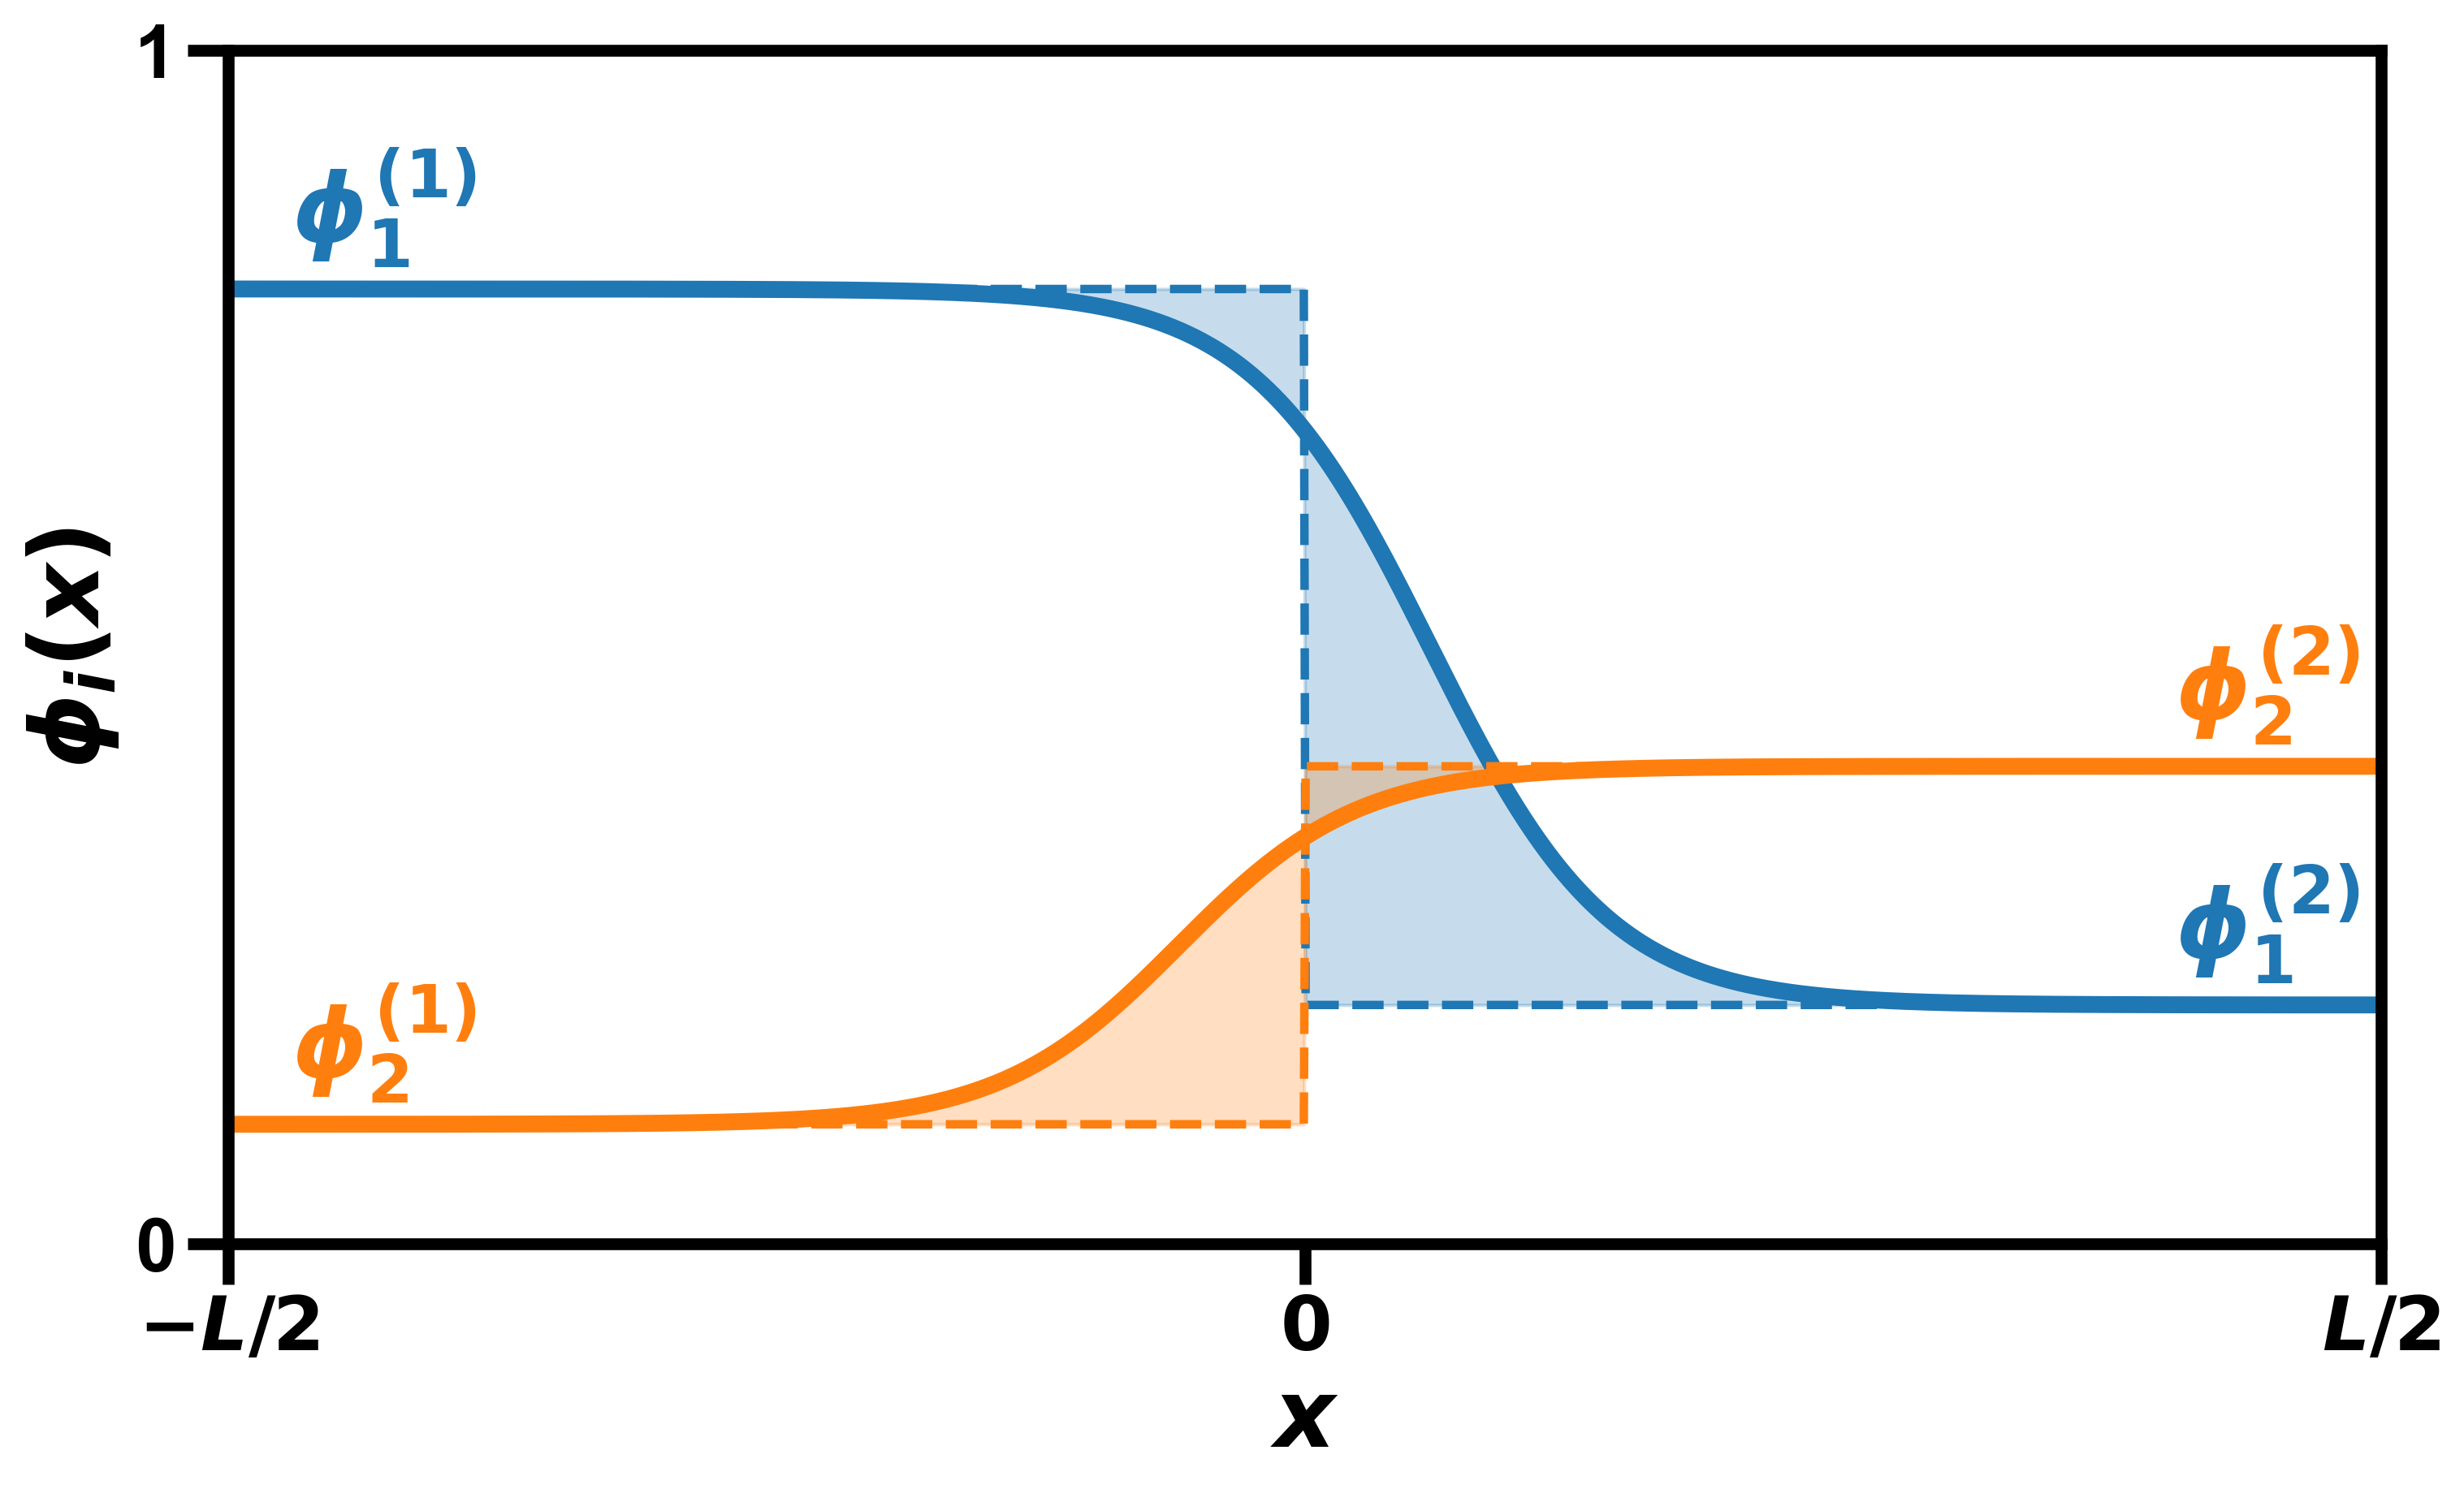
\includegraphics[width=0.98\textwidth]{figures/st_schematic.png}
    \captionof{figure}{Profiles of \(\phi_1(x)\) (blue) and \(\phi_2(x)\) (orange) everywhere. The solid lines show the smooth interfacial profiles, while the dashed lines denote the corresponding hard interface reference profiles with interface position \(x=0\). The shaded areas represent the excess material \(\Gamma_i\), given by the difference between the soft and hard interface profiles.}
    \label{fig:st_schematic}
\end{minipage}\\

Using the definition of the osmotic pressure in Eq.~\eqref{eq:chemical_potential_and_pressure_definitions}, the surface tension can be simplified to
\begin{equation}
\gamma
=
\int_{-L/2}^{L/2} dx\,
\bigg[
f(\phi_1(x),\phi_2(x)) 
-\sum_i \mu_i \phi_i(x) +\Pi
\bigg].
\label{eq:surfacetension_flory}
\end{equation}
where we have used the fact that the osmotic pressures of the coexisting phases are equal, \(\Pi^{(1)} = \Pi^{(2)} = \Pi\).\\
Importantly, the resulting surface tension is independent of the precise choice of interface location. This reflects the fact that the surface tension is a thermodynamic property of the interfacial region as a whole rather than a geometric quantity tied to a particular dividing surface.



\subsection{Numerical methods}

\subsubsection{Euler-Lagrange formalism}

In the previous sections, we derived the kinetics of phase separation from continuity equations and thermodynamic arguments. The stationary solutions of the resulting Cahn-Hilliard equations correspond to equilibrium profiles of the free-energy functional subject to mass conservation. However, solving the Cahn-Hilliard equations numerically can be challenging because they involve fourth-order spatial derivatives.

Alternatively, the equilibrium profiles can be obtained directly from variational calculus by minimizing the free-energy functional with respect to the volume fractions.
This yields the constrained Euler-Lagrange equations 
\[
\frac{\delta F[\phi_1,\phi_2]}{\delta \phi_i(x)} = 0,
\qquad i\in\{1,2\},
\]

The constraints of mass conservation would typically require a Lagrange multiplier on the right-hand side. However, later on we will enforce mass conservation differently.
For a one-dimensional system, the Euler-Lagrange equations take the form
\[
\frac{\partial f}{\partial \phi_i}
-
\partial_x\!\left(\frac{\partial f}{\partial \phi_i'}\right)
=0,
\qquad i\in\{1,2\}.
\]
Inserting the Flory-Huggins free-energy density from Eq.~\ref{eq:fh_free_energy_density} yields the coupled second-order equations
\[
\begin{aligned}
\ln \phi_1 - \ln(1-\phi_1-\phi_2)
+ \tilde\chi_{11}\phi_1 + \tilde\chi_{12}\phi_2
- \tilde\kappa_{11}\phi_1'' - \tilde\kappa_{12}\phi_2''
&=0, \\
\ln \phi_2 - \ln(1-\phi_1-\phi_2)
+ \tilde\chi_{21}\phi_1 + \tilde\chi_{22}\phi_2
- \tilde\kappa_{21}\phi_1'' - \tilde\kappa_{22}\phi_2''
&= 0.
\end{aligned}
\]
These equations can be rearranged into the fixed-point form
\[
\begin{aligned}
\phi_1 &= T_1(\phi_1,\phi_2), \\
\phi_2 &= T_2(\phi_1,\phi_2),
\end{aligned}
\]
where
\[
\begin{pmatrix}
T_1(\phi_1,\phi_2) \\
T_2(\phi_1,\phi_2)
\end{pmatrix}
=
\boldsymbol{\tilde{\chi}}^{-1}
\begin{pmatrix}
\tilde\kappa_{11}\phi_1'' + \tilde\kappa_{12}\phi_2'' - \ln \phi_1 + \ln(1-\phi_1-\phi_2)  \\
\tilde\kappa_{21}\phi_1'' + \tilde\kappa_{22}\phi_2'' - \ln \phi_2 + \ln(1-\phi_1-\phi_2) 
\end{pmatrix}.
\]

This suggests a fixed-point iteration scheme. Since the mapping \(T_i\) is generally not contractive, the naive iteration
\[
\phi_i^{n+1}(x)=T_i(\phi_1^n(x),\phi_2^n(x)),
\qquad i\in\{1,2\},
\]
may oscillate or diverge. Instead, we introduce a pseudo-time relaxation with step size \(0<h\le 1\),
\[
\begin{aligned}
\phi_i^{n+1}(x)
&=
\phi_i^n(x)+h\left[T_i(\phi_1^n(x),\phi_2^n(x))-\phi_i^n(x)\right]\\
&=
\phi_i^n(x)+h\,G_i(\phi_1^n(x),\phi_2^n(x)),\\
\end{aligned}
\]
where
\[
G_i(\phi_1,\phi_2)=T_i(\phi_1,\phi_2)-\phi_i.
\]

To enforce mass conservation of each component at every iteration step, we subtract the spatial average of the update and use
\begin{equation}
\phi_i^{n+1}(x)
=
\phi_i^n(x)
+
h\left[
G_i(\phi_1^n(x),\phi_2^n(x))
-
\left\langle G_i(\phi_1^n,\phi_2^n)\right\rangle_x
\right],
\qquad i\in\{1,2\},
\label{eq:fixed_point_iteration}
\end{equation}
where \(\langle\cdot\rangle_x\) denotes the spatial average. By construction, the spatial average of the update vanishes, so the total mass of each component is conserved throughout the iteration.

This dynamical system is artificial and does not represent the physical evolution of the system. Nevertheless, it relaxes toward the same constrained stationary profiles as the Cahn-Hilliard equations while requiring only the solution of coupled second-order equations instead of fourth-order ones.



\subsubsection{Pseudo-spectral method}

To solve the fixed-point iteration in Eq.~\ref{eq:fixed_point_iteration}, we employ a pseudo-spectral method.
This method is well suited because the second-derivative terms appearing in the Euler-Lagrange equations can be evaluated efficiently in Fourier space, while the nonlinear terms are treated in real space.
Compared with finite-difference or finite-element approaches, spectral methods typically yield much smaller discretization errors for smooth periodic fields and therefore achieve high accuracy with relatively few grid points \cite[Chs.~1.1--1.4]{Boyd2000Chebyshev}

The central idea of the pseudo-spectral method is to use the Fourier transform to convert spatial derivatives into algebraic multiplications in Fourier space. For each component \(i\in\{1,2\}\), the second derivative is computed as
\[
\phi_i''(x)
=
\mathcal{F}^{-1}\!\left[-k^2\,\mathcal{F}[\phi_i(x)]\right],
\]
where \(\mathcal{F}\) denotes the Fourier transform and \(k\) is the wavevector. This allows the second-derivative terms in the operators \(G_i\) to be evaluated efficiently in Fourier space, while the logarithmic and other nonlinear terms are computed pointwise in real space.

Since the pseudo-spectral method relies on Fourier transforms, periodic boundary conditions are required. 
We therefore construct the initial condition by taking a profile with a sharp interface and concatenating it with a flipped copy of itself.
The resulting domain contains two interfaces and is periodic by construction, which avoids discontinuities at the boundaries.

\subsubsection{Semi-implicit stepping scheme}

For diffusion-dominated PDEs, explicit time-stepping schemes can be inefficient because stability imposes a severe restriction on the time step size. For example, the diffusion equation
\[
\frac{d\phi(x,t)}{ dt} = D\,\frac{d^2\phi(x,t)}{dx^2}
\]
requires
\[
\Delta t < \frac{\Delta x^2}{2D}
\]
for stability when discretized with an explicit Euler scheme \cite{Jeong2018StabilityOF}. This restriction arises from the amplification of high-wavevector modes.

A common way to suppress these instabilities is to introduce a semi-implicit stabilization of the update. Instead of using the explicit discretization
\[
\frac{1}{h}\left(\boldsymbol{\phi}^{n+1}-\boldsymbol{\phi}^{n}\right),
\]
we apply the modified operator
\[
\left(\frac{1}{h}-\lambda \partial_{xx}\right)
\left(\boldsymbol{\phi}^{n+1}-\boldsymbol{\phi}^{n}\right),
\]
where \(\lambda>0\) is a stabilization parameter. 

Inserting this into the fixed-point iteration scheme from Eq.~\ref{eq:fixed_point_iteration} and rearranging yields
\begin{equation}
    \phi_i^{n+1}
=
\phi_i^n
+
\frac{h}{1-h\lambda \partial_{xx}}
\left[
G_i(\phi_1^n,\phi_2^n)
-
\langle G_i(\phi_1^n,\phi_2^n)\rangle_x
\right],
\qquad i\in\{1,2\}.
\end{equation}

In Fourier space, the second derivative transforms as \(\partial_{xx} \to -k^2\), so the prefactor becomes
\[
\frac{1}{1+h\lambda k^2}.
\]
Thus, modes with large wavevector \(k\) are strongly damped. This suppresses the short wavelength instabilities that limit explicit schemes and typically allows for much larger time steps.

For \(h\to 0\), the operator \((1-h\lambda\partial_{xx})^{-1}\) approaches the identity and the semi-implicit scheme reduces to the explicit update.

\clearpage
\section{Surface tension of phase interfaces in ternary mixtures}\label{s:surface_tension}
In this chapter, we investigate the surface tension of interfaces in ternary mixtures composed of three components, labeled 0, 1 and 2, with repulsive cross-interactions \(\chi_{ij}>0\).
Without loss of generality, we choose component 2 to have the weakest repulsive interactions with the other two species.
It can accumulate at phase interfaces and therefore partially screen the stronger repulsion between components 0 and 1.

This chapter is organized as follows. We first determine the interfacial profiles and surface tension numerically.
We then introduce a class of approximate interfacial profiles that yields an analytical expression for the surface tension
and show that this approximation retains the correct critical scaling near the critical point.
Next, we compare these predictions with the numerical solutions, to assess the validity and limitations of the approximation and to discuss the role of interfacial adsorption.
Finally, we elucidate the importance of preferential interfacial adsorption by examining the symmetric case.

\subsection{Determining the interfacial profiles and surface tension numerically}\label{sec:interfacial_profiles_numerical}
\subsubsection{Model setup and numerical scheme}
After setting the temperature \(k_B T=1\) and the lattice size \(a=1\) in the free-energy density in Eq.~\eqref{eq:fh_free_energy_density}, the model only depends on the Flory-Huggins interaction matrix \(\tilde\chi_{ij}\).
With the convention used in Eq.~\eqref{eq:fh_free_energy_density}, the gradient coefficient matrix is then
\begin{equation}
    \tilde\kappa_{ij} = -\tilde\chi_{ij}.
\end{equation}
For the purposes of this chapter, we focus on interaction matrices that yield a single interface and therefore avoid parameter regimes with three-phase coexistence, in which multiple interfaces with distinct properties can coexist.

\begin{equation}
    \chi_{12}\in[0.8,1.5],\quad \chi_{02}=1.5, \quad \chi_{01}\in[2.3, 3.0]
    \label{eq:interaction_parameters}
\end{equation}

Accordingly, the parameter range in Eq.~\eqref{eq:interaction_parameters} is chosen to reliably produce liquid-liquid phase separation with two-phase coexistence while, as far as possible, avoiding three-phase coexistence.\\

\noindent
\begin{minipage}{0.45\textwidth}
For a given interaction matrix \(\chi\) and mean compositions \(\bar\phi_1, \bar\phi_2\), we can compute the coexisting phases with the \texttt{flory} package \cite{Yicheng2025flory}.
The coexisting phases are then used to initialize the profiles of each species as two step functions, ensuring periodic boundary conditions at the start of the simulation (see Fig.~\ref{fig:profiles_init}).\\

The grid spacing \(\Delta x\) is set such that the interfacial region spans approximately
\(40\) grid points. The total domain contains \(512\) grid points, which allows the fields to relax to
their bulk values well between the two interfaces.
\end{minipage}
\hfill
\begin{minipage}{0.5\textwidth}
    \centering
    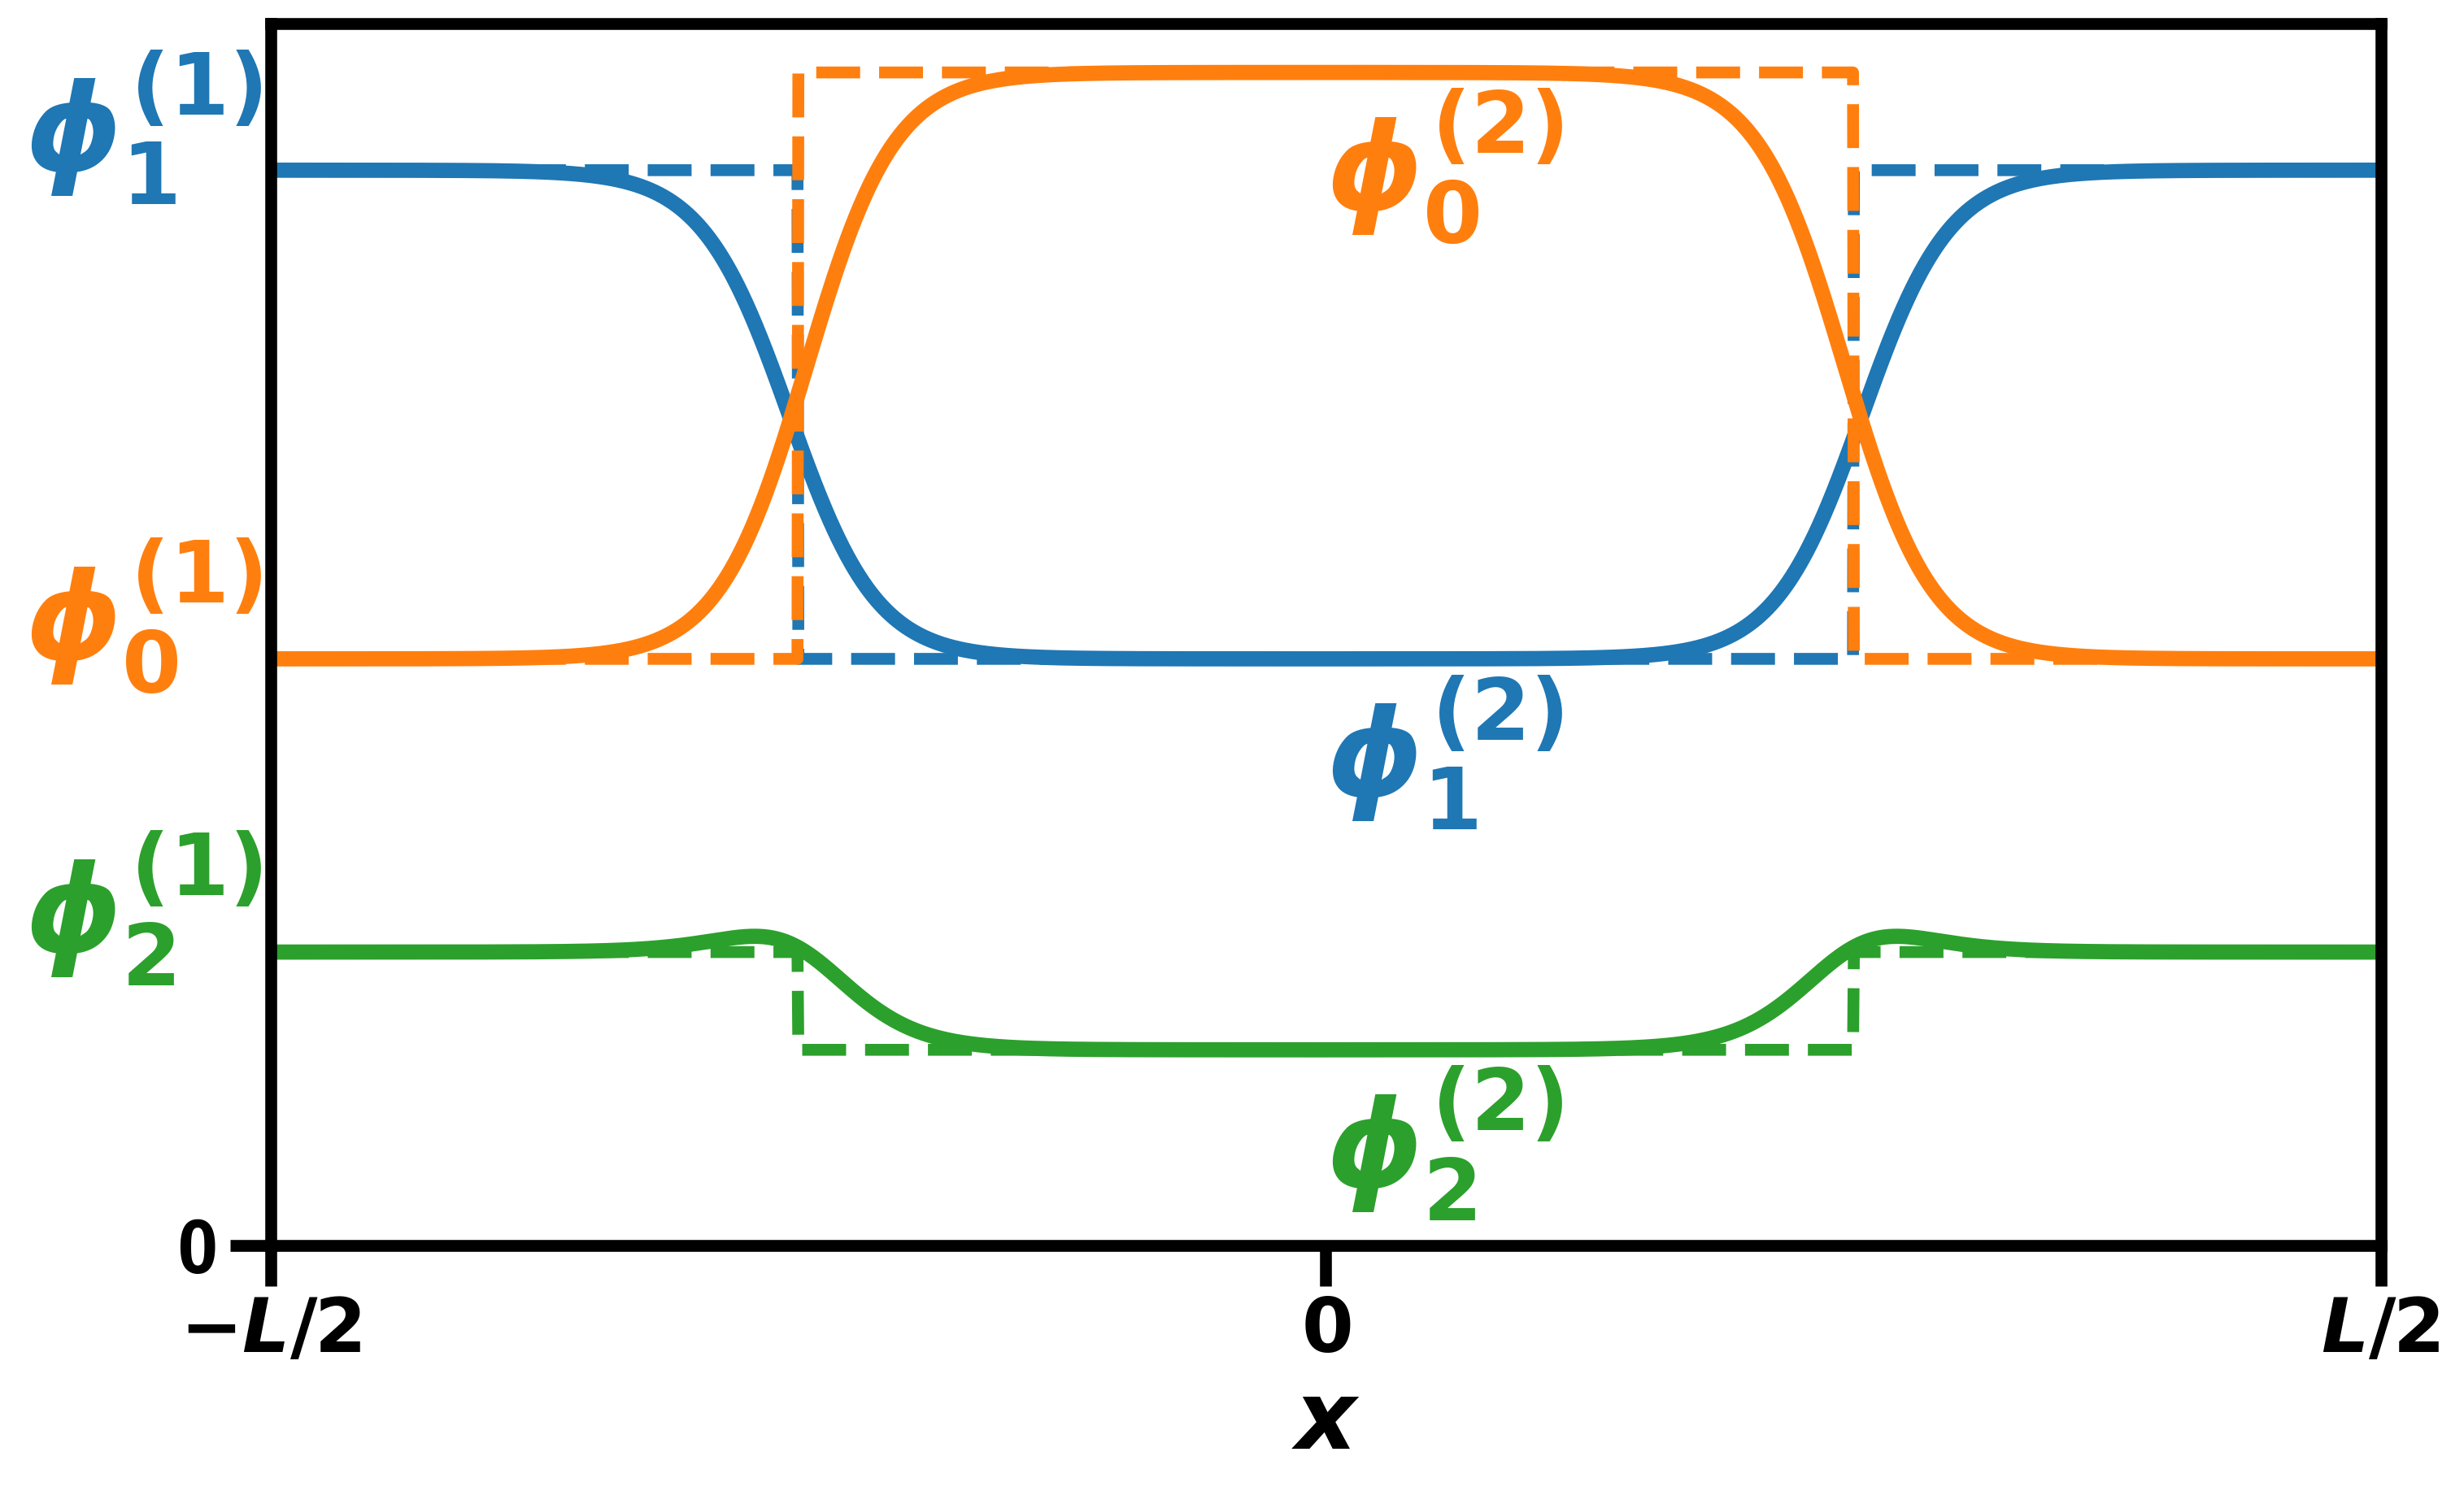
\includegraphics[width=\textwidth]{figures/profiles_init.png}
    \captionof{figure}{Profile initialization: the dashed lines denote the initial profiles and the solid lines the equilibrated profiles. The bulk volume fractions \(\phi_i^{(j)}\) are computed with the \texttt{flory} package \cite{Yicheng2025flory}.}
    \label{fig:profiles_init}
\end{minipage}\\





\subsubsection{Equilibration dynamics and interfacial structure}

Starting from the initial step profile, we relax the system to equilibrium using the fixed-point iteration in Eq.~\eqref{eq:fixed_point_iteration}. Because we are only interested in the equilibrium profiles, the step size \(h\) is chosen as large as numerical stability permits. The semi-implicit update strongly suppresses high-wavenumber modes, allowing us to use \(h=\mathcal{O}(10^{-1})\), typically one to two orders of magnitude larger than in a fully explicit scheme.
Close to the boundary of composition space (\(\bar\phi_2 \sim 0\)), smaller step sizes are required because the logarithmic terms in the free-energy become large and can lead to numerical instabilities.

We declare convergence when the maximum change of the two-phase compositions \(\boldsymbol\phi =(\phi_1^{(1)}\,\phi_2^{(1)},\phi_1^{(2)}\,\phi_2^{(2)})^T\) between two iterations satisfies
\[
\max_x\, \lVert \boldsymbol{\phi}^{n+1}(x)-\boldsymbol{\phi}^{n}(x)\rVert < 10^{-10}.
\]
Depending on the interaction parameters and initialization, this criterion is reached after \(10^4\)-\(10^5\) iterations.
Repeating this equilibration for increasing \(\bar\phi_2\) allows us to track the interfacial profiles up to the critical point,
beyond which two-phase coexistence is no longer possible (Fig.~\ref{fig:workflow}).



\noindent
\begin{minipage}{0.95\textwidth}
    \centering
    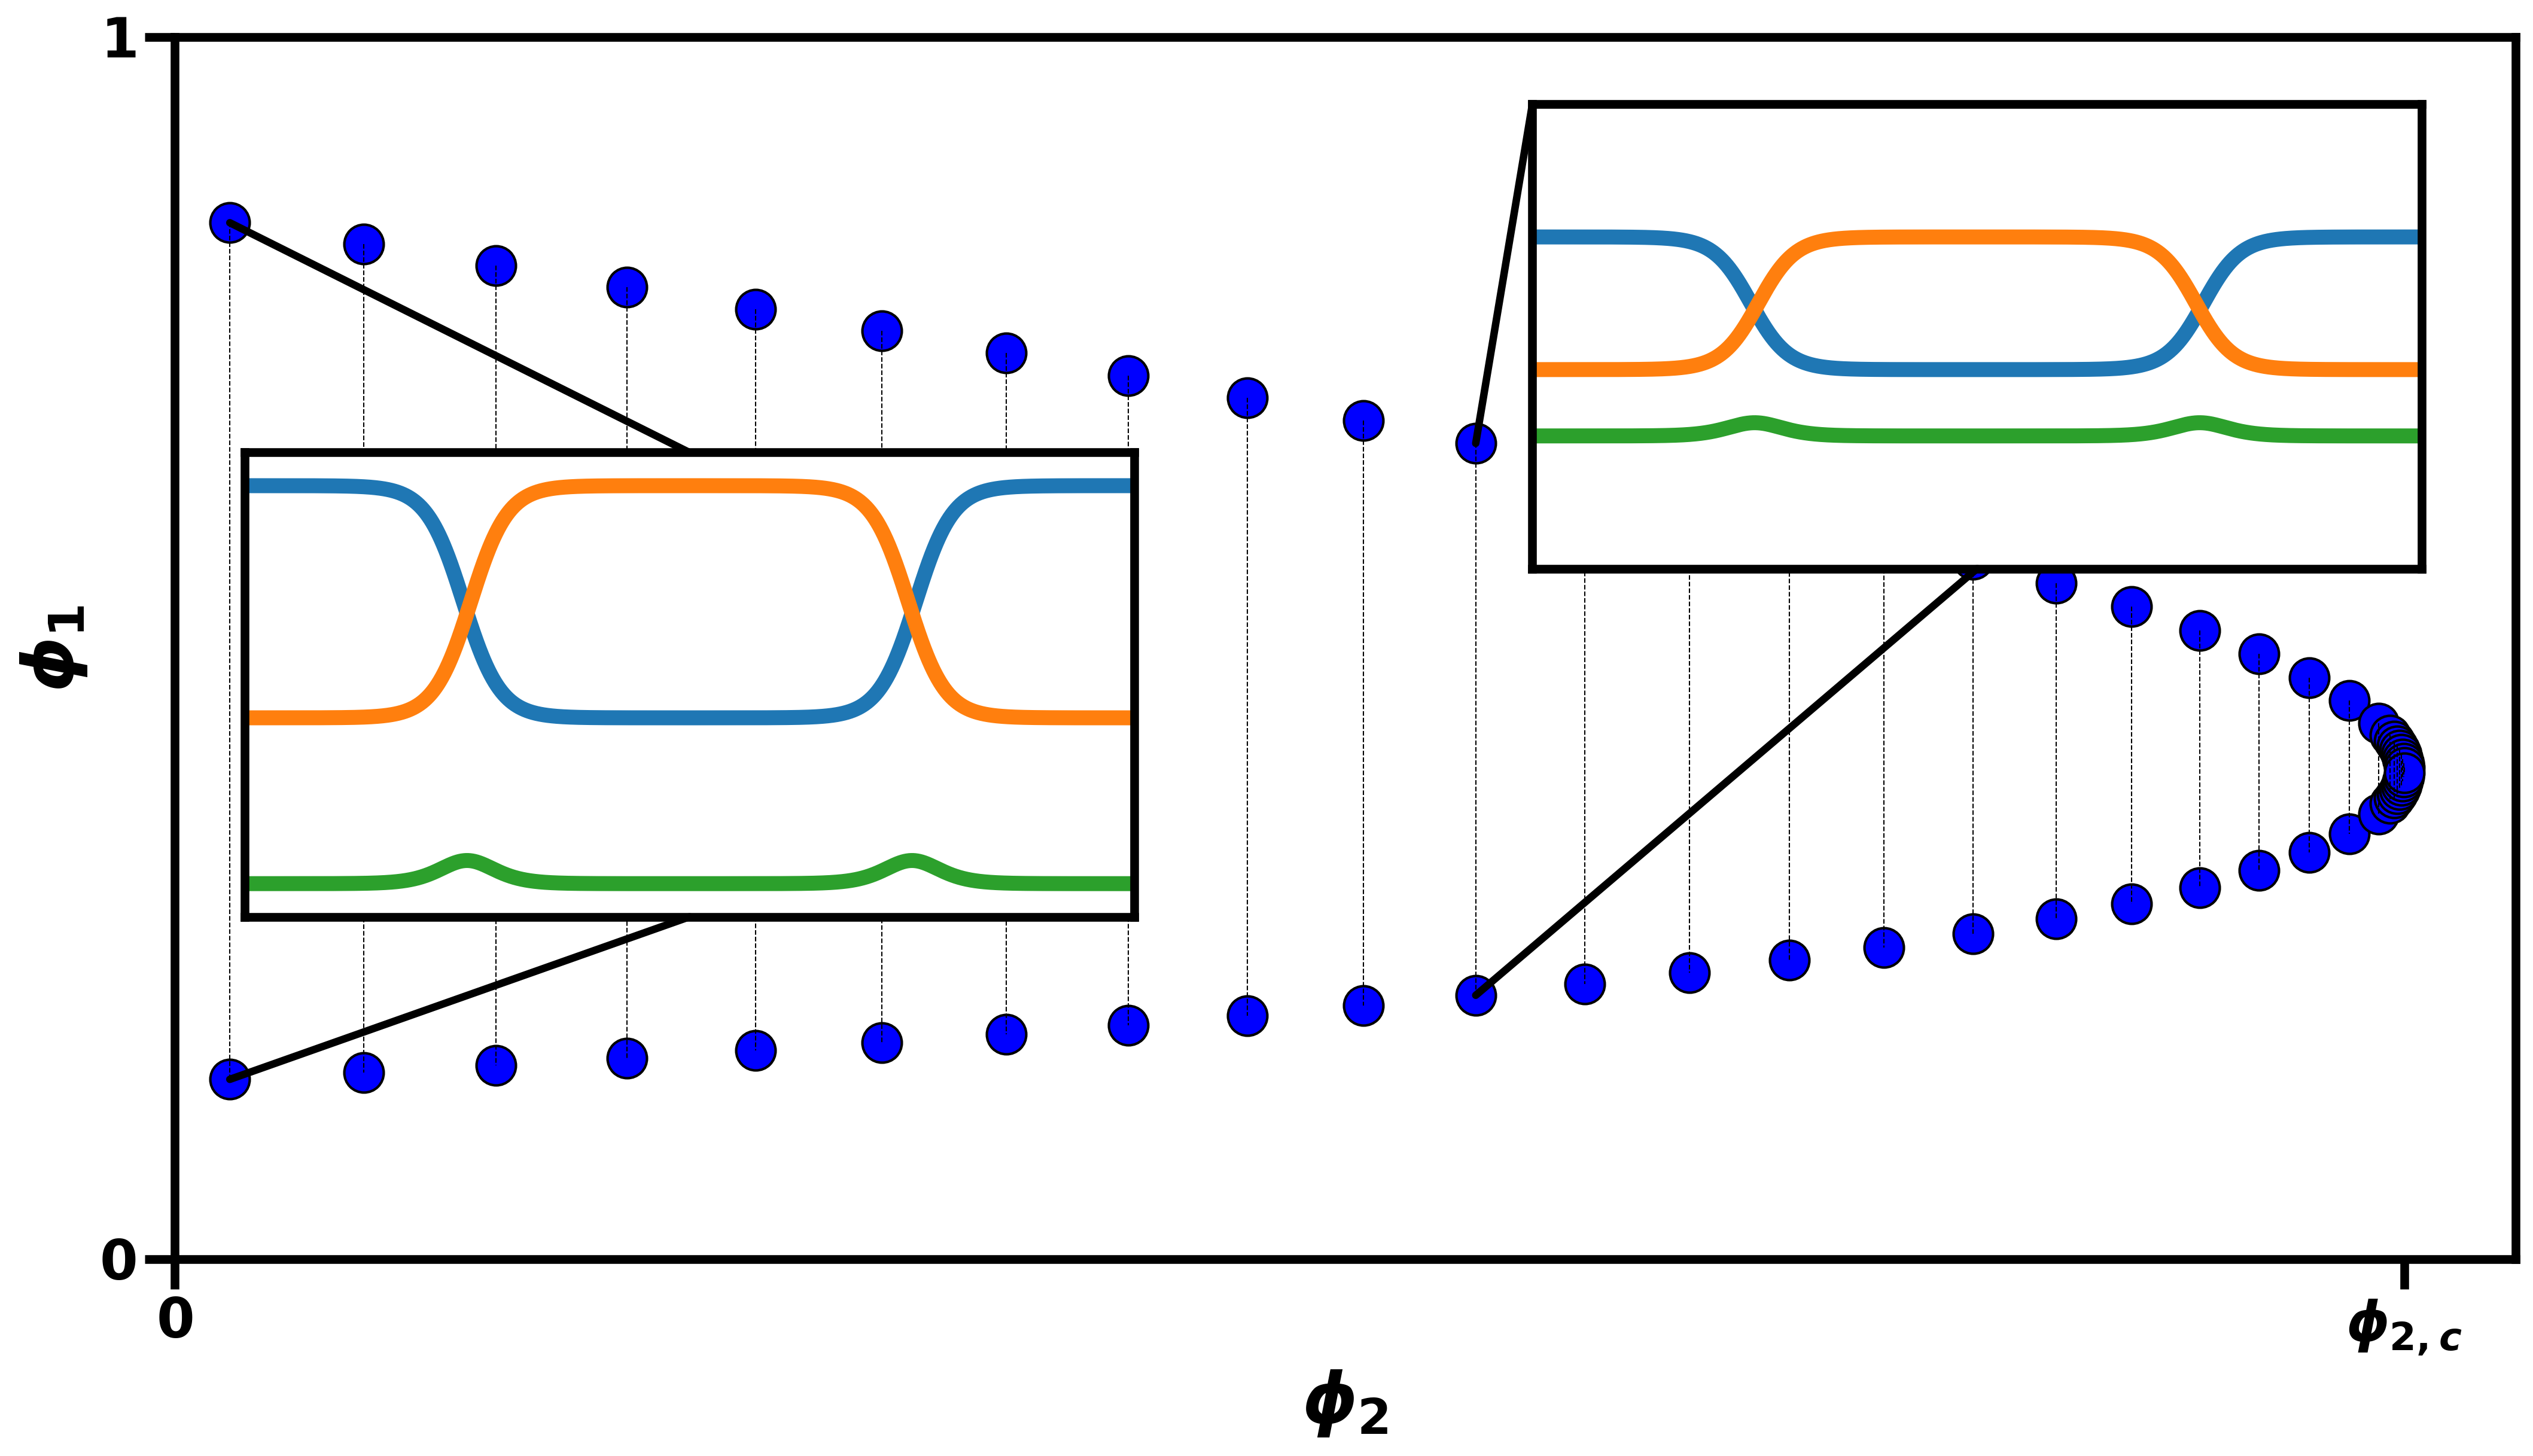
\includegraphics[width=\textwidth]{figures/workflow_chapter_two.png}
    \captionof{figure}{Workflow: Selecting volume fractions along the binodal in phase space (blue dots) and then equilibrating the interfacial profiles (insets).
    Starting from the dilute limit (\(\bar\phi_2\sim 0\)), we repeat this procedure until the critical point is reached.}
    \label{fig:workflow}
\end{minipage}\\

At equilibrium, components \(0\) and \(1\) vary smoothly across the interface, whereas species \(2\) may become enriched there. This is intuitive, as its accumulation screens the strongest repulsive interactions between species \(0\) and \(1\).

This adsorption becomes more pronounced as \(\chi_{01}\) increases and, for sufficiently strong repulsion between species \(0\) and \(1\), may even promote the appearance of a third phase.
This trend is consistent with the symmetric case \(\chi_{02} = \chi_{12}\) studied in \cite{Huang1999}, where the interfacial adsorption of species \(2\) was found to scale with \(\chi_{01}/\chi_{12}\).


\subsubsection{Critical scaling of the surface tension}
\textcolor{red}{Perhaps add a figure in supplement showing numerical fit of simulation data to power law and resulting critical exponent.}
After obtaining the equilibrium profiles, we compute the surface tension using the derived expression in Eq.~\eqref{eq:surfacetension_flory}.
In this way, we collect surface-tension values along the binodal for different mean volume fraction of species 2.
In the following we will display the surface-tension as a function of the distance to the critical chemical potential \(\mu_{2,c}-\mu_2\) of species 2.
The chemical potential relates to the volume fraction \(\phi_2\) through Eq.~\eqref{eq:chemical_potential_and_pressure}.
The critical point is then located at \(\mu_{2,c}=\mu_2(\phi_{2,c})\).
The results for the surface tensions are shown in Fig.~\ref{fig:surface_tension_numerical}.



\noindent
\begin{minipage}{\textwidth}
    \centering
    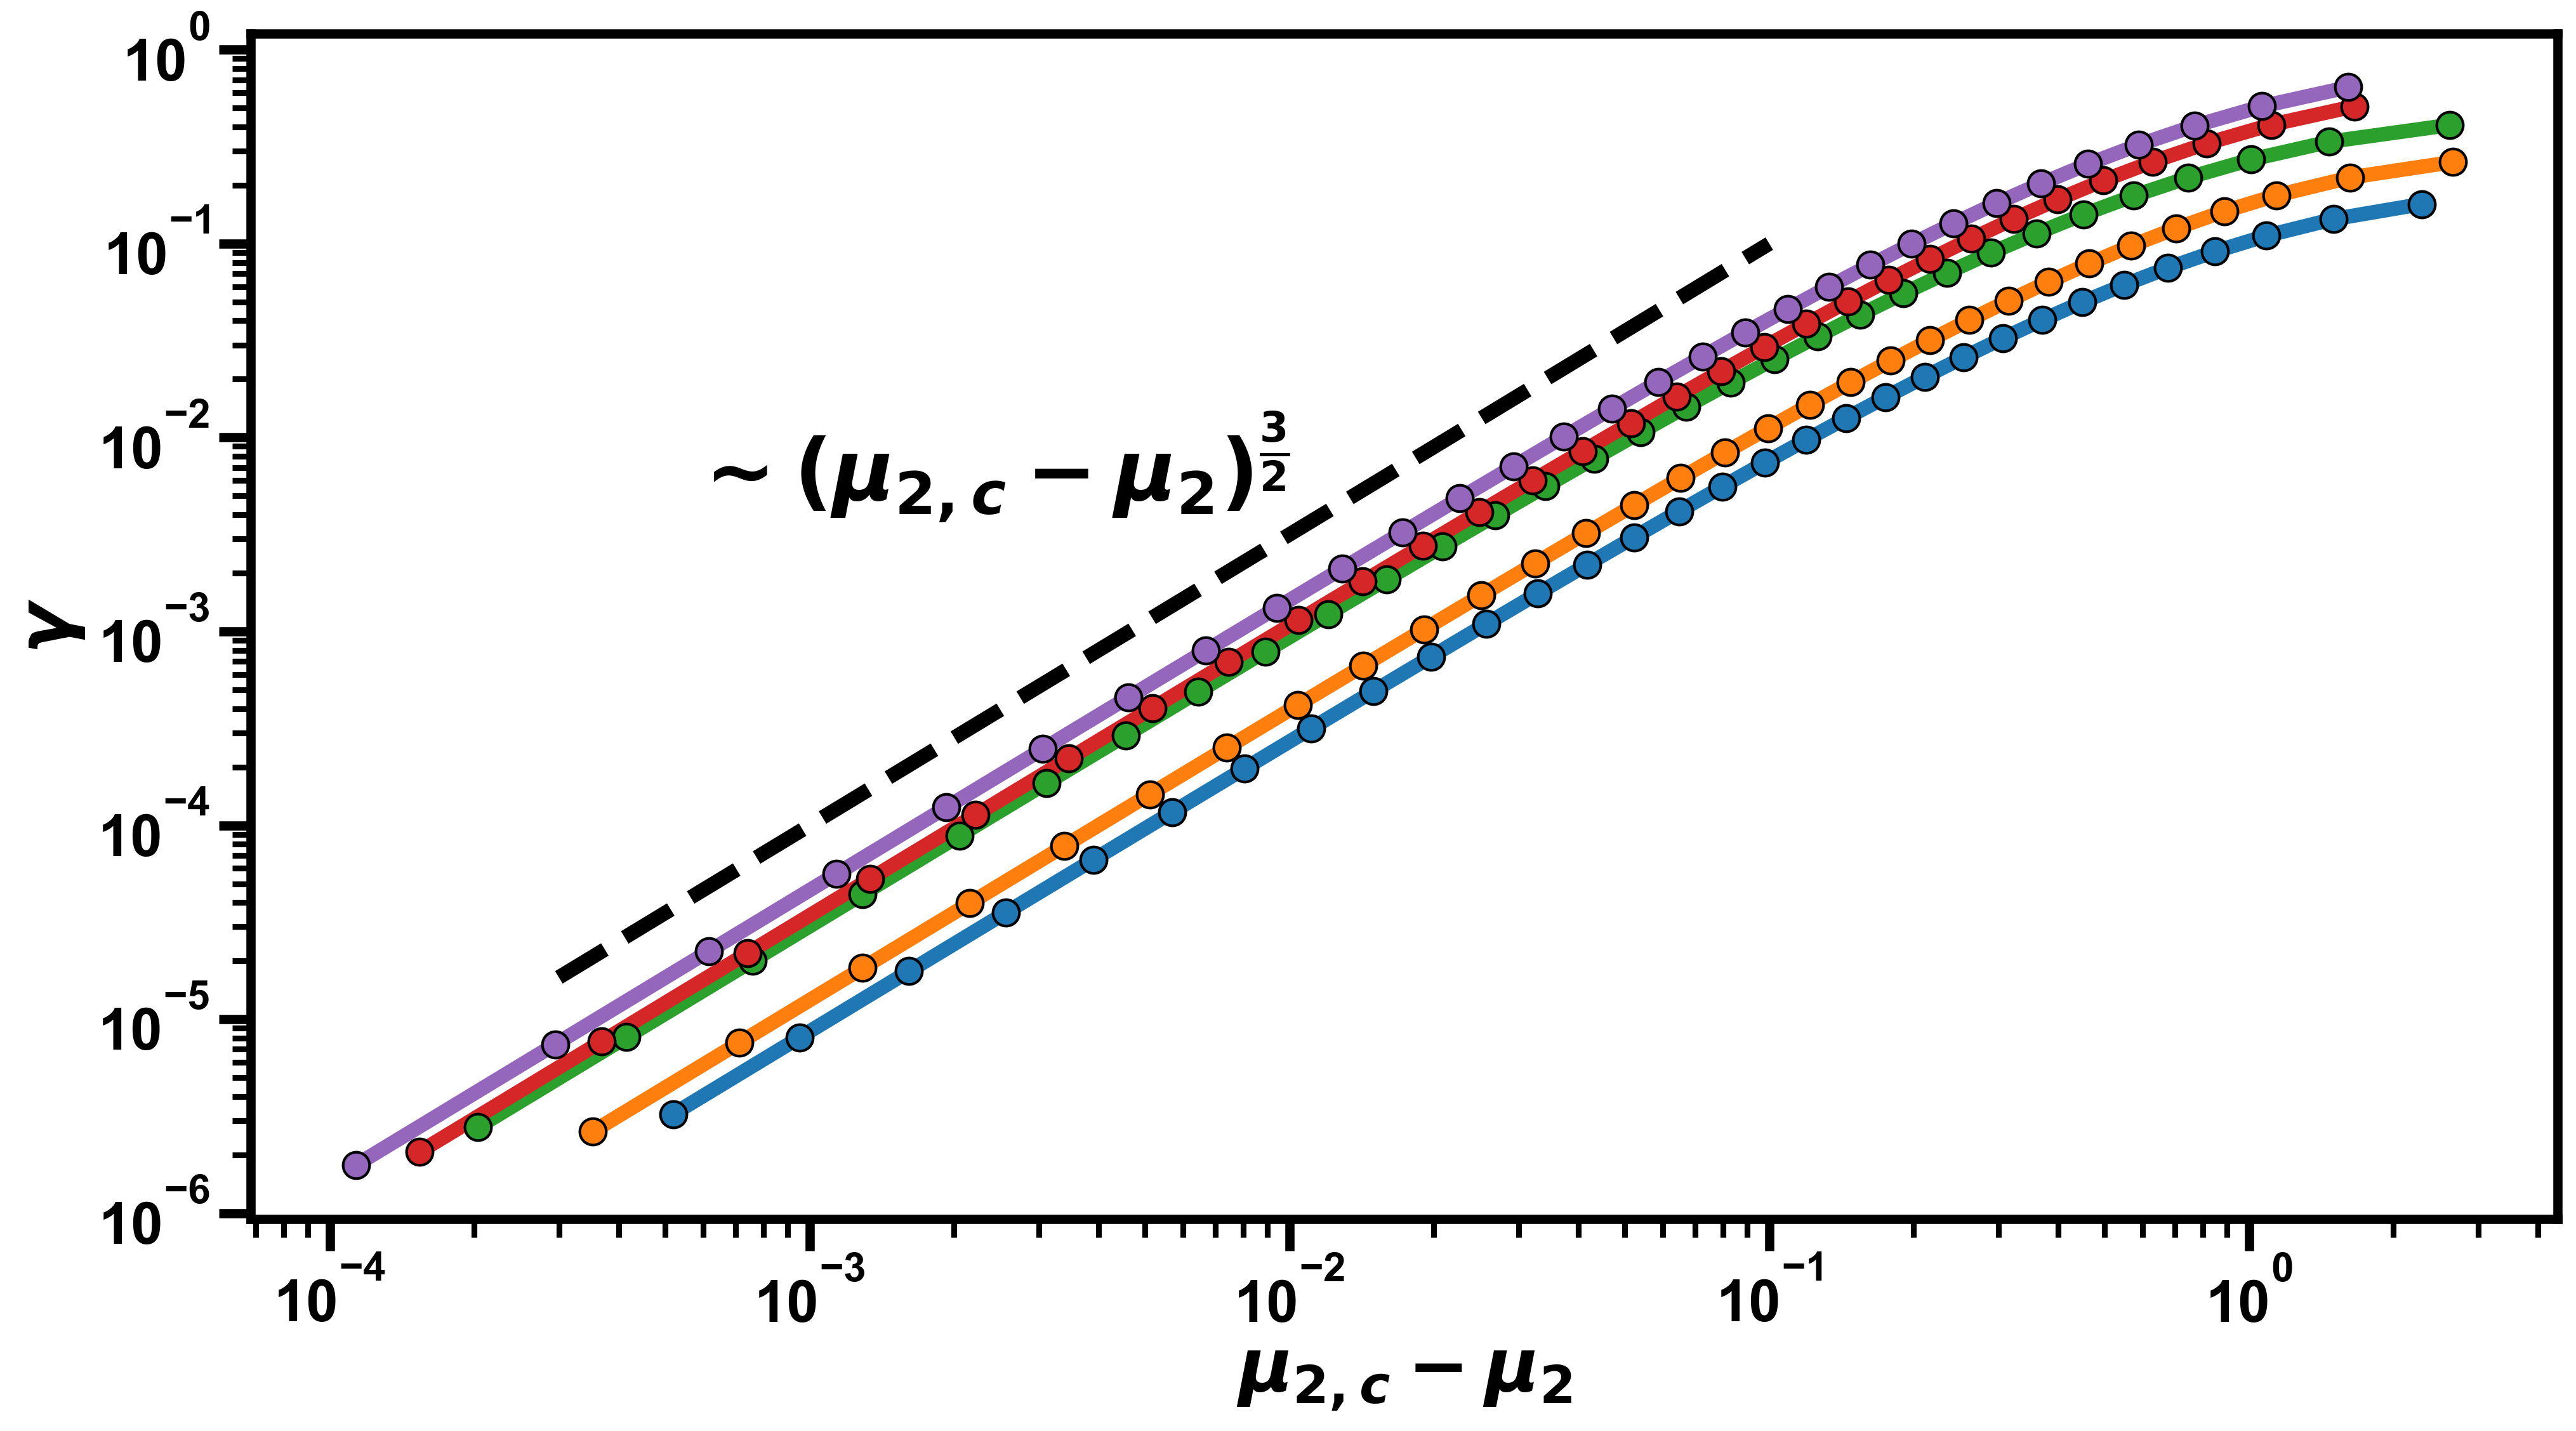
\includegraphics[width=0.95\textwidth]{figures/st_simulation_results.png}
    \captionof{figure}{Surface tension as a function of the chemical potential distance to the critical point, \(\mu_{2,c}-\mu_2\),
    for various interaction parameters (colored lines) in the range specified by Eq.~\eqref{eq:interaction_parameters}.
    Close to criticality, the surface tension exhibits the power-law scaling \(\gamma \sim (\mu_{2,c}-\mu_2)^{3/2}\) (dashed line).\\}
    \label{fig:surface_tension_numerical}
\end{minipage}

As the system approaches the critical point, the two coexisting phases merge continuously and the surface tension vanishes.

Close to criticality, we observe a clear power-law dependence of the surface
tension on the chemical potential difference, \(\mu_{2,c}-\mu_2\):
\[
\gamma \sim (\mu_{2,c}-\mu_2)^{\frac{3}{2}}.
\]
This scaling is essentially the same for all interaction parameters considered.

To quantify this behavior, we fit the numerical data close to criticality to the form
\[
\gamma = A(\mu_{2,c}-\mu_2)^{\delta},
\]
where \(A\) is a prefactor and \(\delta\) is the critical exponent. These fits yield \(\delta \approx 3/2\) within numerical uncertainty.
\footnote{The fitted critical exponent typically deviates by more than \(0.1\) from \(3/2\) if points farther than \(10^{-2}\) from the critical point are included in the fit.}

Additionally, the critical exponent is consistent with previous work \cite{Huang1996AnalyticInterface}. In contrast, the prefactor of the power law
is not universal and varies substantially with the choice of interaction
parameters (nearly an order of magnitude in Fig.~\ref{fig:surface_tension_numerical}).



\subsection{An effective interfacial model to approximate the surface tension}

While the critical scaling of the surface tension near the critical point is physically insightful, because it separates universal critical behavior from the non-universal prefactor set by the interaction parameters, obtaining a closed-form expression for $\gamma$ from the full ternary Flory-Huggins free-energy appears, as far as we know, to be intractable.


Consequently, for each choice of interaction parameters and mean compositions, the surface
tension must be computed by solving the full numerical interfacial problem, as has been done in Section~\ref{sec:interfacial_profiles_numerical}.\\




\noindent
\begin{minipage}{0.6\textwidth}

To avoid this computational cost, we now introduce an analytical approximation that
estimates the surface tension using only the bulk volume fractions of the coexisting
phases and the interaction parameters, thereby removing the need to equilibrate the spatially extended system.
The approximation provides good qualitative agreement over a broad range of interaction parameters and reproduces the
correct scaling near the critical point, as we will demonstrate later.

\subsubsection{Derivation of a piecewise-linear interface}

As shown in the previous sections, interfacial profiles in ternary mixtures can be
highly nontrivial (see Fig.~\ref{fig:approx_intuition}A). To obtain an analytically tractable approximation, we represent
the interface by a piecewise-linear profile that connects the two coexisting bulk
phases over a finite interfacial width. In this approximation, all species share the same
interfacial width, as illustrated in Fig.~\ref{fig:approx_intuition}B.\\
This approximation relies on two nontrivial assumptions. First, it ignores the intrinsic nonlinearity of the equilibrium profiles.
Second, by enforcing a common interfacial window for all components, it rules out interfacial adsorption, since the accumulation of one species would shift the others relative to it along the $x$-axis.
We discuss the implications of these assumptions later.\\

To derive the approximation for the surface tension, we will
first identify a conserved quantity of the equilibrium interfacial problem. For a
one-dimensional interface at equilibrium, the Euler-Lagrange equations imply the
existence of a quantity that is constant across the interface.\\
Writing the free-energy density as a sum of a local and a gradient
contribution and adopting Einstein summation convention, we define
\begin{equation}
    f(\{\phi_i(x)\})
    = f_{\mathrm{local}}(\{\phi_i(x)\})
    + \frac{1}{2}\, \phi_i'(x)\,\tilde\kappa_{ij}\, \phi_j'(x).
\end{equation}
\end{minipage}
\hfill
\begin{minipage}{0.35\textwidth}
    \centering
    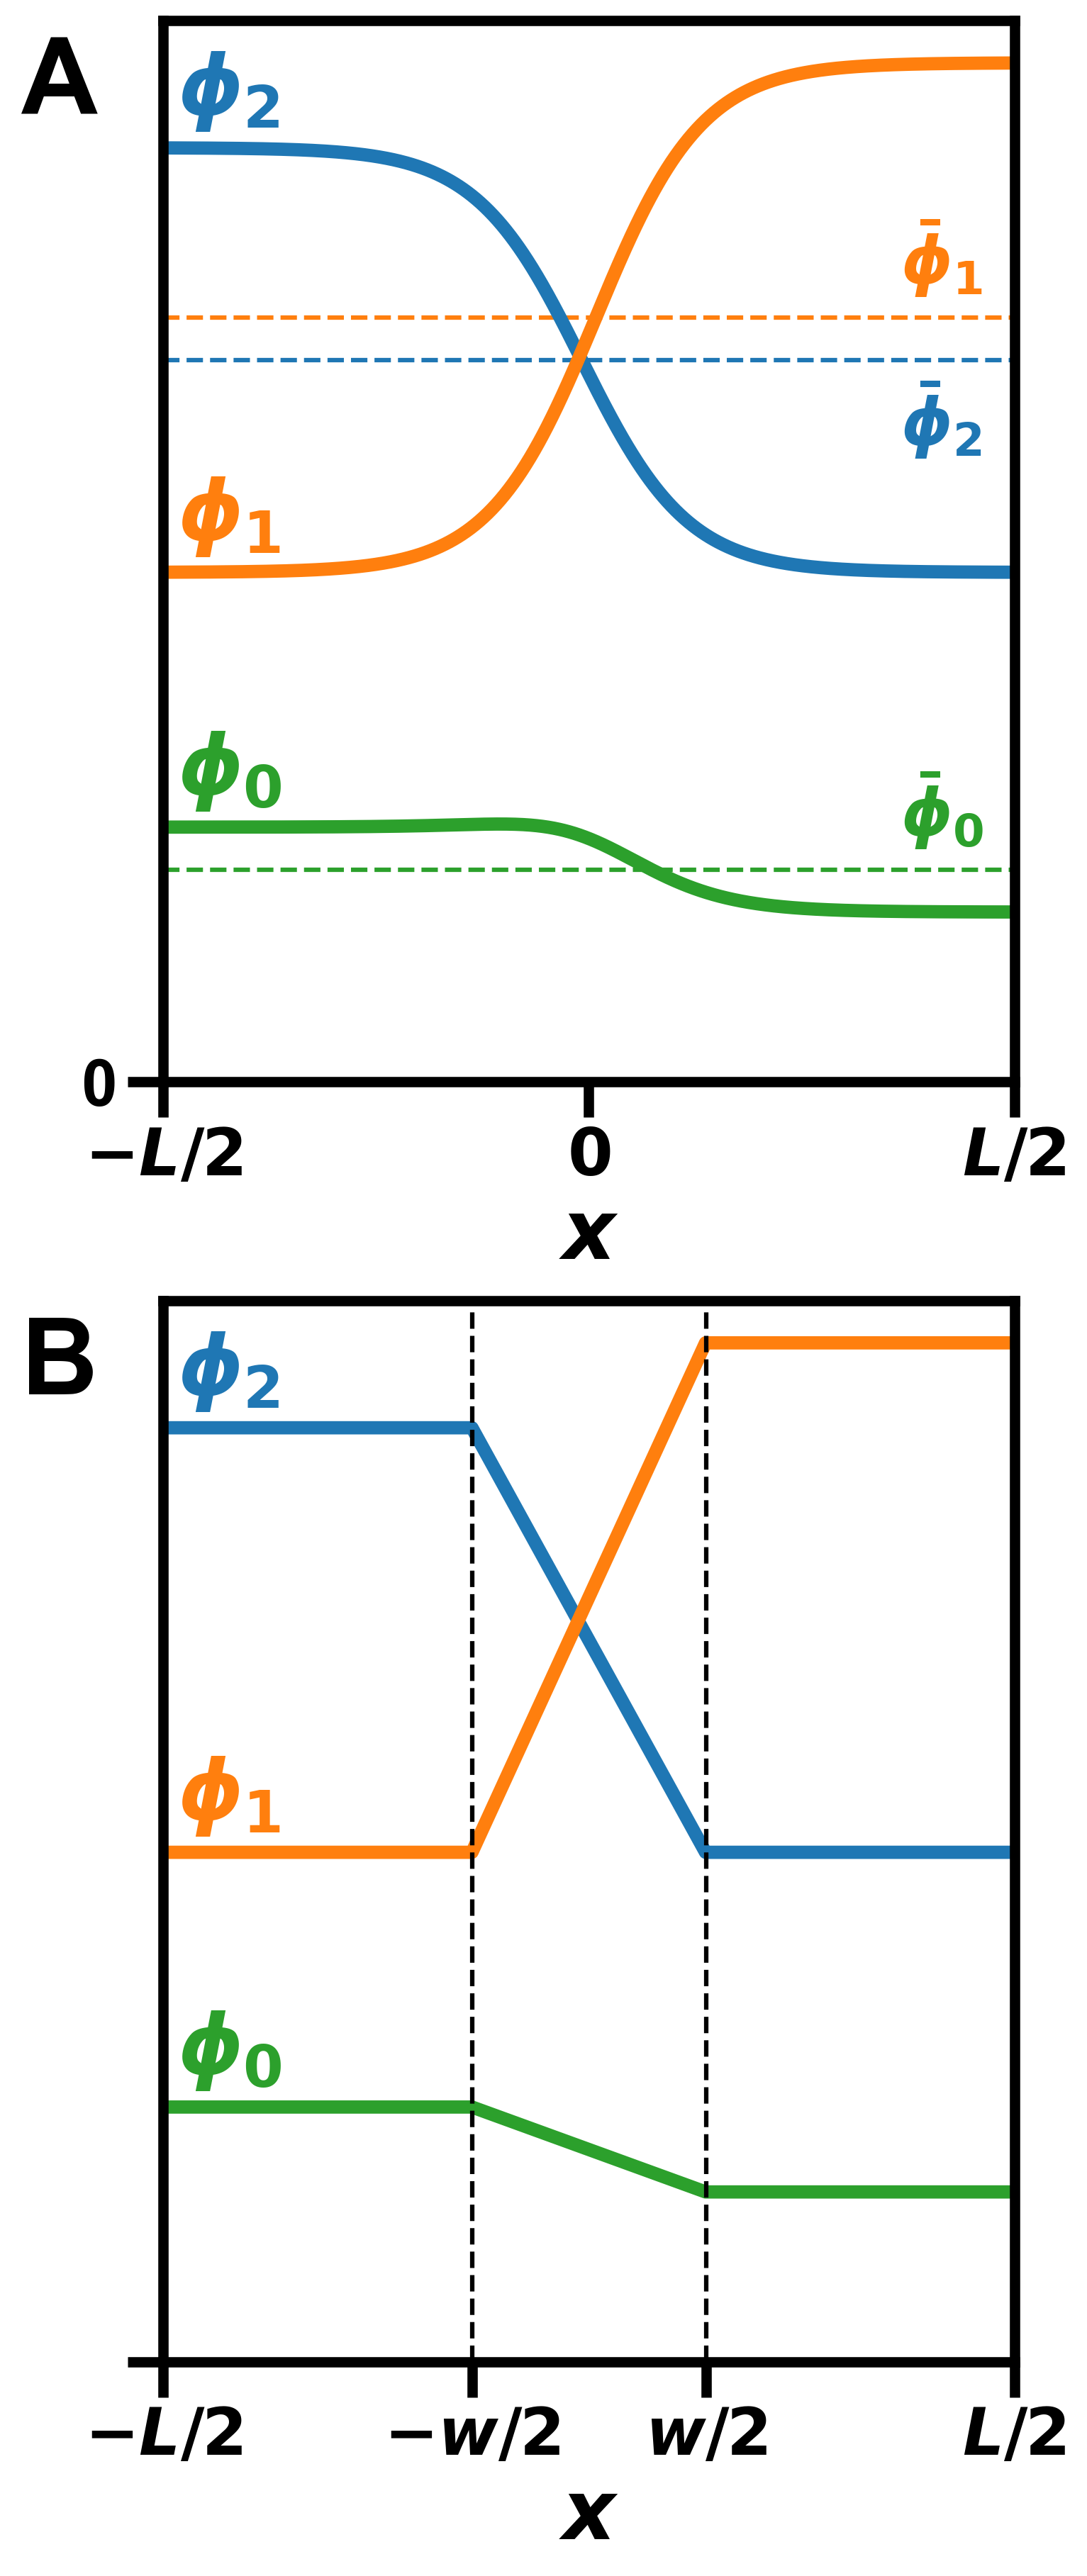
\includegraphics[width=\textwidth]{figures/approximation_intuition.png}
    \captionof{figure}{(A) Schematic of the true interfacial profile (solid lines) compared with (B) the piecewise-linear approximation. The dashed horizontal lines in (A) denote the midpoint compositions \(\bar\phi_i\). The dashed vertical lines in (B) indicate the interfacial width \(w\).}
    \label{fig:approx_intuition}
\end{minipage}\\

Introducing the exchange chemical potentials $\mu_i$ and osmotic pressure $\Pi$, the
combination

\begin{equation}
    0=f_{\mathrm{local}}(\{\phi_i(x)\})
    - \mu_i \phi_i(x)
    + \Pi
    - \frac{1}{2}\, \phi_i'(x)\,\tilde\kappa_{ij}\, \phi_j'(x)
    \eqcolon -V(\{\phi_i(x)\}) - T(\{ \phi_i'(x)\})
    \label{eq:invariant_quantity}
\end{equation}

vanishes everywhere. Here, the terms $V$ and $T$ play roles analogous
to potential and kinetic energy in classical mechanics.

To verify this invariance, we take the spatial derivative of Eq.~\eqref{eq:invariant_quantity}, which yields

\[
\begin{aligned}
    \frac{d}{dx} \Bigl(
    f_{\mathrm{local}}(\{\phi_i\})
    - \mu_i \phi_i
    + \Pi
    - \frac{1}{2}\, \phi_i'(x)\,\tilde\kappa_{ij}\, \phi_j'(x)
    \Bigr)
    &=
    \left(
    \frac{\partial f_{\mathrm{local}}}{\partial \phi_i}
    - \mu_i
    - \tilde\kappa_{ij}  \phi_j''(x)
    \right)
    \frac{d\phi_i}{dx} \\
    &= 0,
\end{aligned}
\]

where the expression in parentheses vanishes by virtue of the Euler–Lagrange
equations. Consequently, we have found a conserved quantity in Eq.~\eqref{eq:invariant_quantity}.
\textcolor{red}{Should I move this to the first chapter?}\\


We now return to the piecewise-linear approximation.
% Its simplicity comes at the
% cost of two important assumptions. First, by imposing a common interfacial window
% for all components, it excludes adsorption at the interface, since the accumulation
% of one species would shift the profiles of the others relative to one another along
% the \(x\)-axis. Second, it neglects the intrinsic nonlinearity of the equilibrium
% profiles. We will discuss the implications of these assumptions later on.
Within the approximation, each component varies linearly across an interface of width $w$,
connecting the bulk values $\phi_i^{(1)}$ and $\phi_i^{(2)}$ for $i \in \{1,2\}$. The magnitude of the
gradient at the interface \(x=0\) is therefore given by (see Fig.~\ref{fig:approx_intuition})
\[
    | \phi_i'(0)|= \frac{|\Delta \phi_i|}{w},
\]
where $\Delta \phi_i = \phi_i^{(1)} - \phi_i^{(2)}$ denotes the difference between the
coexisting bulk phases and \(\phi_i'(0)\) is the gradient at the interface.

Substituting the gradient approximation into the quadratic gradient term
yields
\[
      {\phi}_i'(0)\, \tilde\kappa_{ij}\,  \phi_j'(0)
    =
    w^{-2}\,\Delta \phi_i\, \tilde\kappa_{ij}\, \Delta \phi_j.
\]
Solving for the interfacial width gives
\begin{equation}
    w
    =
    \sqrt{
    \frac{
        \Delta \phi_i\, \tilde\kappa_{ij}\, \Delta \phi_j
    }{
        \phi_i'(0)\, \tilde\kappa_{ij}\, \phi_j'(0)
    }
    }.
    \label{eq:interface_width_initial}
\end{equation}
Next, we can substitute the expression in the denominator using the invariant quantity from Eq.~\eqref{eq:invariant_quantity}:
\begin{equation}
        \phi_i'(0)\, \tilde\kappa_{ij}\, \phi_j'(0) = 2\left(
        f_{\mathrm{local}}(\{\phi_i(0)\})
        - \mu_i \phi_i(0)
        + \Pi
        \right)
    \label{eq:gradient_substitution}
\end{equation}
In this approximation, the volume fractions at the interface are equal to the midpoint compositions
\[
    \phi_i(0)=\bar{\phi}_i = \frac{1}{2}\left(\phi_i^{(1)} + \phi_i^{(2)}\right),
\]

Plugging Eq.~\eqref{eq:gradient_substitution} into Eq.~\eqref{eq:interface_width_initial} yields the final expression for the interfacial width:
\begin{equation}
    w
    =
    \sqrt{
    \frac{
        \Delta \phi_i\, \tilde\kappa_{ij}\, \Delta \phi_j
    }{
        2\left(
        f_{\mathrm{local}}(\{\bar{\phi}_i\})
        - \mu_i \bar{\phi}_i
        + \Pi
        \right)
    }}
    \label{eq:interface_width_approximation}
\end{equation}

Next we will derive the corresponding approximation for the surface tension.
The surface tension is given by Eq.~\eqref{eq:surfacetension_flory}:

\[
\begin{aligned}
\gamma
&=
\int_{-L/2}^{L/2} dx\,
\bigg[
f(\{\phi_i(x)\}) 
-\sum_i \mu_i \phi_i(x) +\Pi
\bigg]\\
    &=\int_{-L/2}^{L/2} dx\, \phi_i'(x)\, \tilde\kappa_{ij}\, \phi_j'(x)
\end{aligned}
\]

where in the second equality we used the invariant quantity from Eq.~\eqref{eq:invariant_quantity}.

Within the linear-profile approximation, the gradients are constant across the
interface and vanish in the bulk. The integral therefore reduces to

\[
    \gamma_\mathrm{approx}
    =
    w\, \phi_i'(0)\, \tilde\kappa_{ij}\, \phi_j'(0),
\]

Substituting the expression for $w$ from
Eq.~\eqref{eq:interface_width_approximation} yields the approximate surface tension

\begin{equation}
    \gamma_\mathrm{approx}
    =
    \sqrt{
    2\left(
        \Delta \phi_i\, \tilde\kappa_{ij}\, \Delta \phi_j
    \right)
    \left(
        f_{\mathrm{local}}(\{\bar{\phi}_i\})
        - \mu_i \bar{\phi}_i
        + \Pi
    \right)
    }
    \label{eq:surface_tension_approximation}
\end{equation}

As anticipated, this expression depends only on \(\Delta\phi_i\) and the midpoint compositions \(\bar\phi_i\), which in turn depend
on the bulk compositions \(\{\phi_i^{(1)}, \phi_i^{(2)}\}\) of the coexisting phases.
Importantly, the closed-form nature of
Eq.~\eqref{eq:surface_tension_approximation} allows derivatives of the surface
tension with respect to the bulk phase compositions to be evaluated analytically.

The quantitative comparison between the analytical approximation and the numerical
results is shown in Fig.~\ref{fig:approximation_compare}.\\

\begin{minipage}{\textwidth}
    \centering
    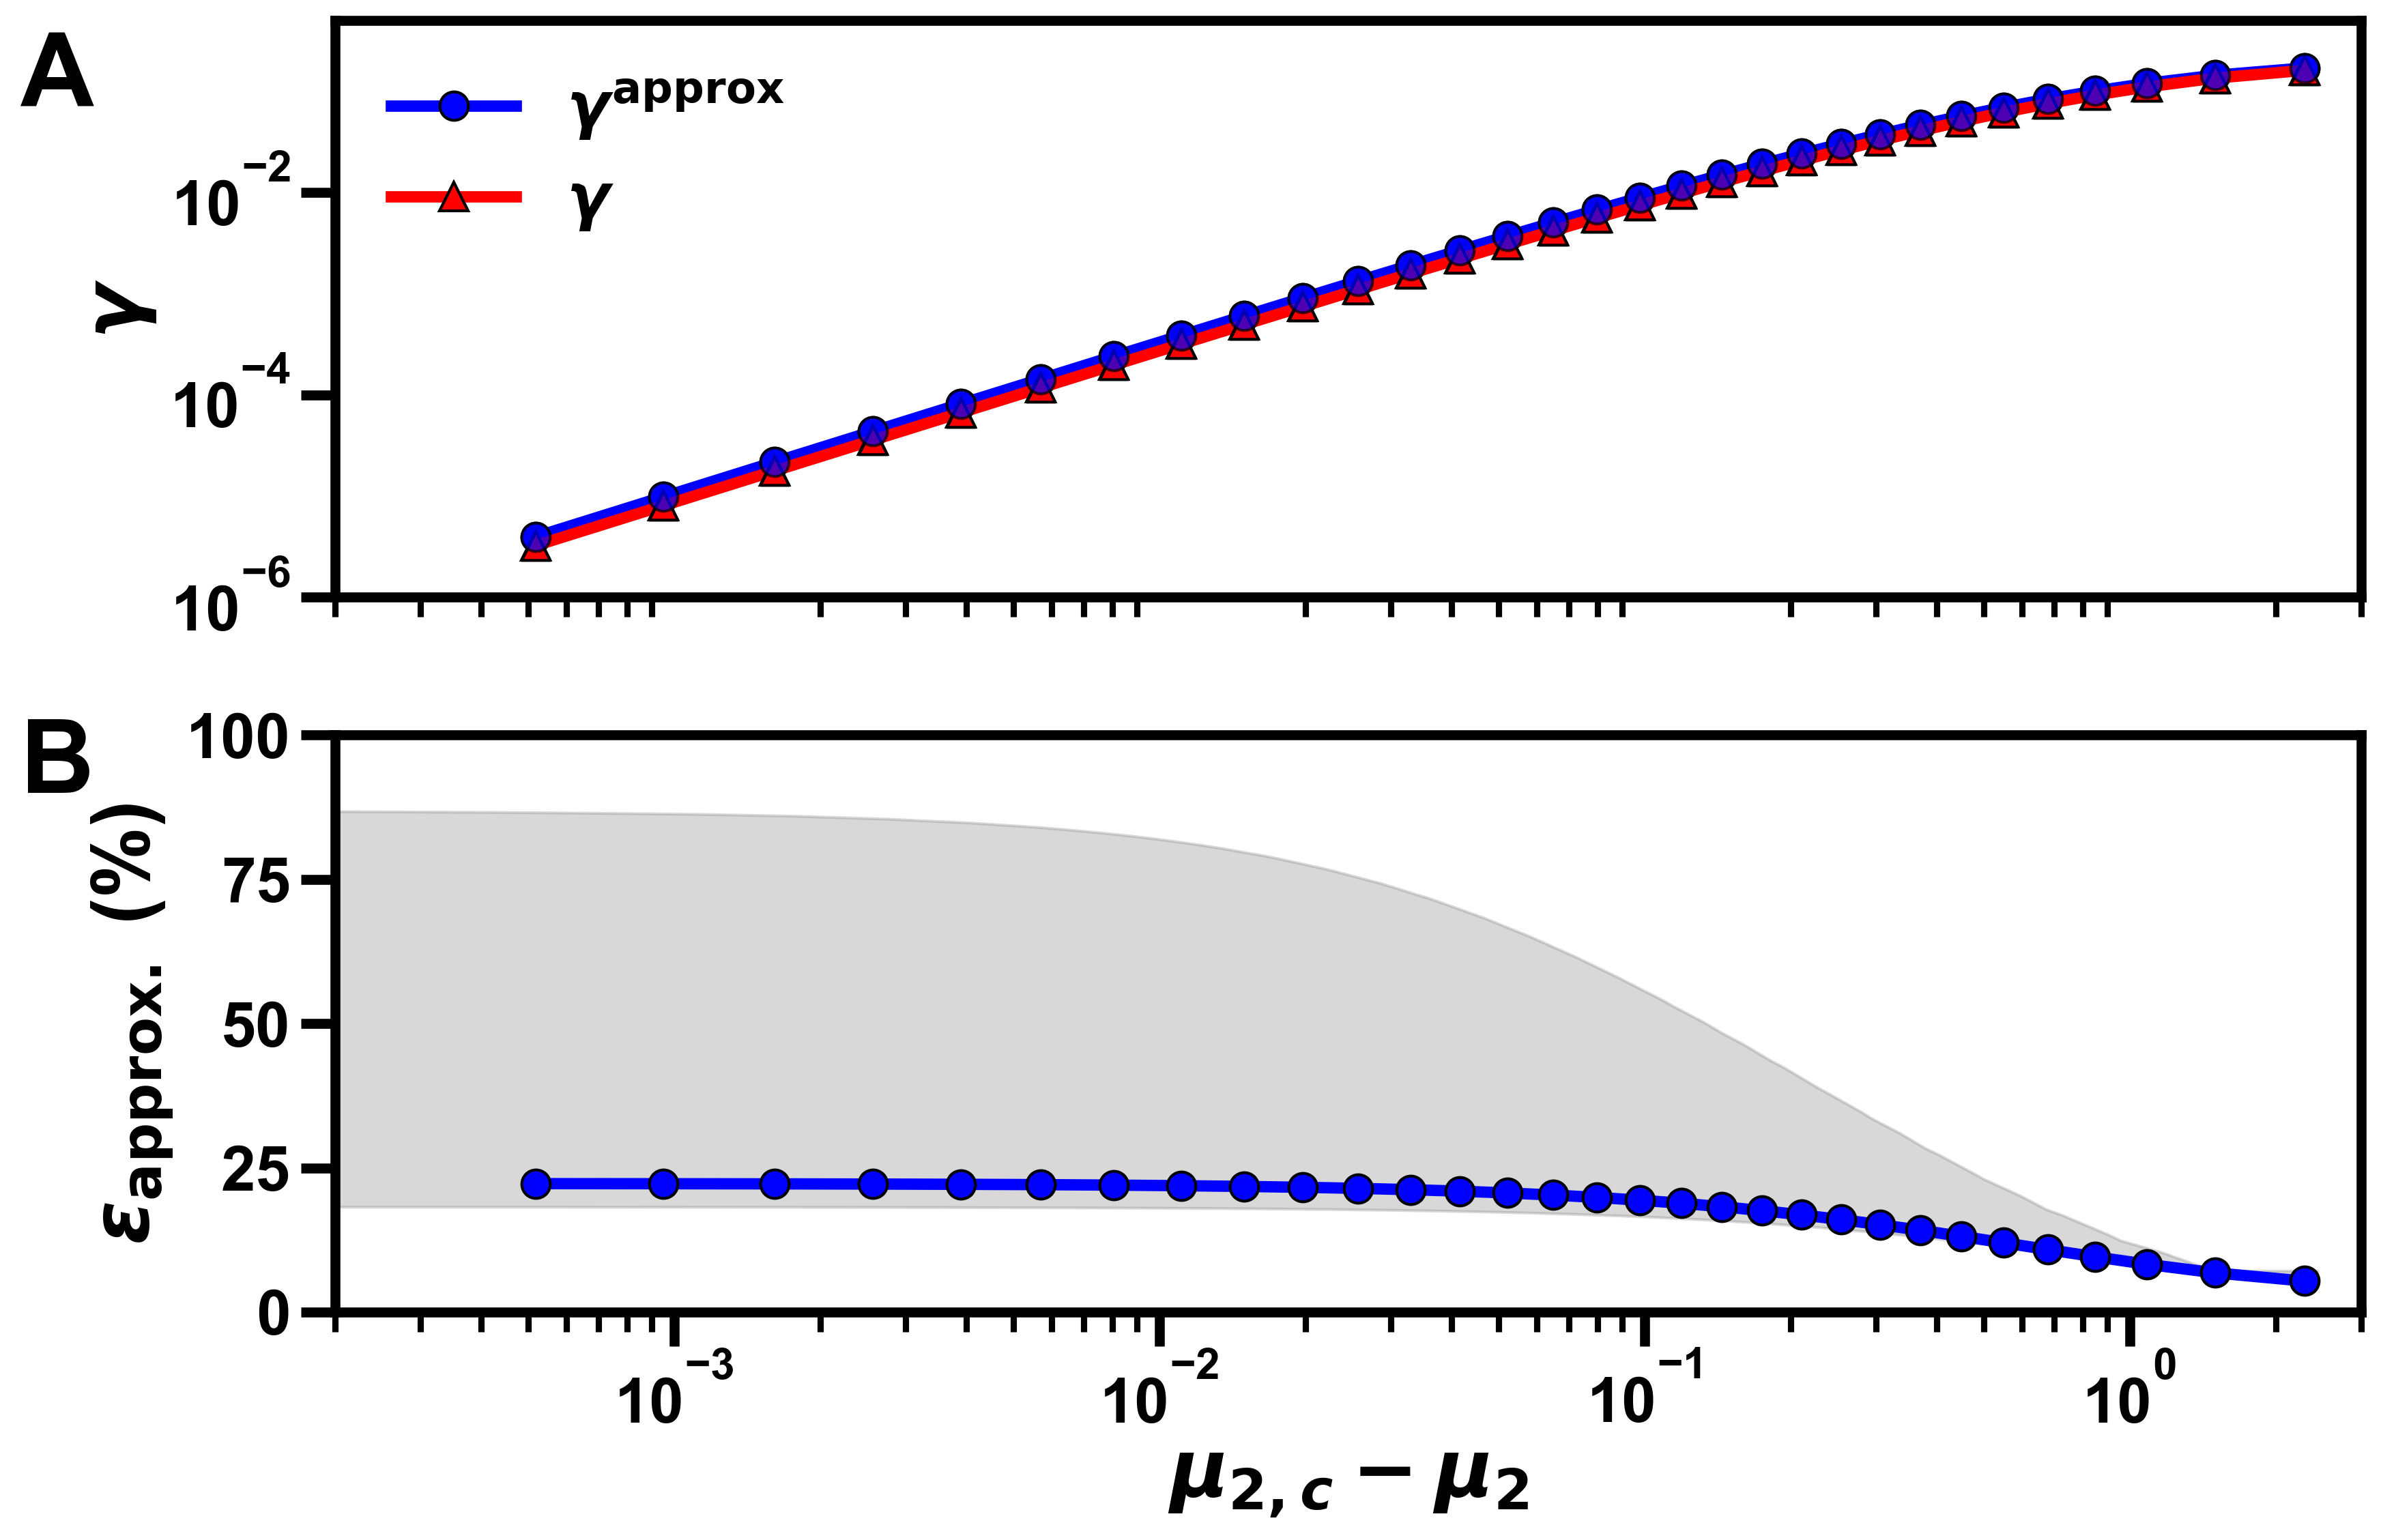
\includegraphics[width=0.95\textwidth]{figures/approximation_compare.png}
    \captionof{figure}{(A) Exact (red) and approximate (blue) surface tension for \(\chi_{01}=1.4\), \(\chi_{02}=1.5\), \(\chi_{12}=2.5\)
    as a function of the chemical potential.
    (B) Relative error \(\epsilon_\mathrm{approx} =(\gamma_{\mathrm{approx}}-\gamma_{\mathrm{exact}})/\gamma_{\mathrm{exact}}\), where the blue data points correspond to the same parameters as in (A) and the gray area indicates the range of errors obtained for the other interaction parameters in Eq.~\eqref{eq:interaction_parameters}.\\}

    \label{fig:approximation_compare}
\end{minipage}\\

Despite its simplicity, the approximate expression not only reproduces the correct
critical scaling but also provides good qualitative agreement with the numerically
computed surface tension over a wide range of parameters.
For the parameter range considered in Eq.~\eqref{eq:interaction_parameters}, the relative error ranges from roughly \(20\%\) to \(90\%\),
as shown in Fig.~\ref{fig:approximation_compare} (gray area).
Additionally, one can see that the approximation becomes more accurate as the system approaches the dilute limit (large values of \(\mu_{2,c}-\mu_2\)).

A systematic deviation is nevertheless apparent: the analytical approximation
overestimates the exact surface tension. The origin of this bias can be understood
from the variational structure of the interfacial problem.
Using the invariant quantity from Eq.~\eqref{eq:invariant_quantity}, the effective
Lagrangian density of the system can be identified as

\[
    L = T - V = 2T =  \phi_i'(x) \,\tilde\kappa_{ij}\,  \phi_j'(x),
\]


where $T$ and $V$ denote the gradient and local contributions, respectively. The
surface tension can therefore be interpreted as the action associated with the
interfacial profile,

\[
    \gamma = \int dx\, L \equiv S.
\]

Since the true equilibrium interface minimizes this action, any approximate
interfacial profile necessarily yields a larger value of $\gamma$. The systematic
overestimation observed in the analytical approximation is thus a direct
consequence of the underlying variational principle.



\subsubsection{Asymptotic critical scaling}

In the previous section, we showed that the surface tension can be expressed
approximately in terms of the bulk compositions of the coexisting phases. We now
analyze the behavior of this expression in the vicinity of the critical point, with
the goal of deriving its asymptotic scaling form.
To do so, we analyze the two factors in the square root in Eq.~\eqref{eq:surface_tension_approximation} separately and then combine their critical scalings.

We first consider the first factor in the square root

\[
    \Delta \phi_i \,\tilde\kappa_{ij}\, \Delta \phi_j,
\]

which depends solely on the difference between the bulk compositions of the two
coexisting phases.


In the following, we switch to vector notation, where for example \(\boldsymbol \mu = (\mu_1\, \mu_2)^T\).
Expanding the chemical potentials in the two coexisting phases about the critical
point yields

\begin{equation}
    \boldsymbol{\mu}^{(\alpha)} - \boldsymbol{\mu}_c
    =
    \boldsymbol{H}\,\Delta\boldsymbol{\phi}^{(\alpha)} + \mathcal{O}(\Delta \phi^2),\quad \alpha \in \{1,2\},
\end{equation}

where $\boldsymbol{H}$ denotes the Hessian of the local free-energy density evaluated
at the critical composition and
$\Delta\boldsymbol{\phi}^{(\alpha)} = \boldsymbol{\phi}^{(\alpha)} - \boldsymbol{\phi}_c$.
At coexistence, the chemical potentials in the two phases must be equal,
$\boldsymbol{\mu}^{(1)}=\boldsymbol{\mu}^{(2)}$. Subtracting the expansions for the two phases and
defining

\[
    \Delta \boldsymbol{\phi}
    =
    \Delta \boldsymbol{\phi}^{(1)} - \Delta \boldsymbol{\phi}^{(2)},
\]

we obtain, to leading order,

\begin{equation}
    \boldsymbol{H}\,\Delta \boldsymbol{\phi} = 0 .
    \label{eq:hessian_null_space}
\end{equation}

This shows that the difference between the bulk compositions of the coexisting
phases lies in the null space of the Hessian at the critical point.

Furthermore, in the immediate vicinity of the critical point, the binodal is
approximately a straight line. Consequently, the deviations
$\Delta \boldsymbol{\phi}^{(1)}$ and $\Delta \boldsymbol{\phi}^{(2)}$ are parallel to $\Delta \boldsymbol{\phi}$ and
thus also belong to the null space of $\boldsymbol{H}$. As a result, the linear term
in the Taylor expansion of the chemical potentials vanishes along the coexistence
direction and higher-order terms control the leading behavior near criticality.


Since \(\Delta \boldsymbol{\phi}^{(1)}\) and \(\Delta \boldsymbol{\phi}^{(2)}\) are parallel to \(\Delta \boldsymbol{\phi}\), the second-order contribution to the Taylor expansion of the chemical potentials can be expressed in terms of \(\Delta \boldsymbol{\phi}\) as follows:

\begin{equation}
 \boldsymbol{\mu}^{(\alpha)} - \boldsymbol{\mu}_c
    =
    \frac{1}{2}
    \left(\alpha^{(\alpha)}\right)^2
    \left[
        \frac{\partial^2 \mu_i}{\partial \phi_j \partial \phi_k}\bigg\rvert_{\boldsymbol{\phi_c}}
        \,\Delta \phi_j \Delta \phi_k
    \right]\boldsymbol{e}_i
    + \mathcal{O}(\Delta \phi^3),\quad \alpha \in \{1,2\},
    \label{eq:second_order}
\end{equation}

where we use Einstein summation convention and we have
introduced

\[
    \alpha^{(1)}
    =
    \frac{\lvert \Delta \boldsymbol{\phi}^{(1)} \rvert}
         {\lvert \Delta \boldsymbol{\phi} \rvert}, \quad \alpha^{(2)}
    =
    \frac{\lvert \Delta \boldsymbol{\phi}^{(2)} \rvert}
         {\lvert \Delta \boldsymbol{\phi} \rvert}.
\]

Since the chemical potentials must again be equal in the two coexisting phases,
$\boldsymbol{\mu}^{(1)}=\boldsymbol{\mu}^{(2)}$, the prefactors must satisfy
$\left(\alpha^{(1)}\right)^2=\left(\alpha^{(2)}\right)^2$. Additionally, the two phases
must have displacements with opposite sign along the tie-line, which implies

\[
    \Delta \boldsymbol{\phi}^{(1)}
    =
    -\,\Delta \boldsymbol{\phi}^{(2)}
    =
    \frac{1}{2}\,\Delta \boldsymbol{\phi}.
\]

The sum inside the brackets in Eq.~\eqref{eq:second_order} is generally nonzero.
Consequently, the leading-order contribution to the chemical potential deviation is of second order:

\[
    \lvert \boldsymbol{\mu}_c-\boldsymbol{\mu} \rvert
    \sim
    \lvert \Delta \boldsymbol{\phi} \rvert^2 .
\]

This relation is consistent with the numerical results shown in Fig.~\ref{fig:factor_scaling}A, where $\lvert \Delta \boldsymbol{\phi} \rvert^2$ is plotted against the chemical potential difference $\lvert \boldsymbol{\mu}_c-\boldsymbol{\mu} \rvert$ on a log-log scale.\\

We now turn to the second factor in the surface-tension approximation. To determine its scaling, we first rewrite it in a convenient form, then expand the free-energy and chemical-potential contributions separately, and finally collect the leading terms.

The second factor can be rewritten as

\begin{equation}
    f(\bar{\boldsymbol{\phi}})
    -\sum_i \mu_i \bar{\phi}_i
    + \Pi
    =
    f(\bar{\boldsymbol{\phi}})
    - f(\boldsymbol{\phi}^{(1)})
    +\sum_i \mu_i \bigl(\phi_i^{(1)} - \bar{\phi}_i\bigr),
    \label{eq:second_product}
\end{equation}

where in the second equality we evaluate the pressure at $\boldsymbol \phi = \boldsymbol \phi^{(1)}$.
For convenience, we write the local free-energy density as $f_\mathrm{local} = f$.

We begin with the free-energy term. Close to the critical point, the dense-phase composition is approximately
\[
    \phi_i^{(1)} \approx \phi_{i,c} + \frac{1}{2}\,\Delta \phi_i ,
\]
while the midpoint composition satisfies
\[
    \bar{\phi}_i
    =
    \frac{1}{2}\bigl(\phi_i^{(1)} + \phi_i^{(2)}\bigr)
    \approx
    \phi_{i,c},
\]
where the last equality follows from the approximately linear shape of the binodal near the critical point, which implies \(\Delta \boldsymbol{\phi}^{(1)} \approx -\Delta \boldsymbol{\phi}^{(2)}\).

We now expand the local free-energy density about the critical composition
$\boldsymbol{\phi}_c$. Using Einstein summation convention, we obtain
\begin{equation}
    \begin{split}
        f(\boldsymbol{\phi}^{(1)})
        &=
        f(\boldsymbol{\phi}_c)
        + \frac{1}{2}\,\mu_{i,c}\,\Delta \phi_i
        + \frac{1}{2^2\,2!}\,
        \Delta \phi_i \underbrace{H_{ij}\bigg\rvert_{\boldsymbol{\phi_c}}\,\Delta \phi_j}_{=\,0} \\
        &\quad
        + \frac{1}{2^3\,3!}\,
        \underbrace{
        \frac{\partial^3 f}{\partial \phi_i \partial \phi_j \partial \phi_k}\bigg\rvert_{\boldsymbol{\phi_c}}
        \Delta \phi_i \Delta \phi_j \Delta \phi_k
        }_{=\,0} \\
        &\quad
        + \frac{1}{2^4\,4!}\,
        \frac{\partial^4 f}{\partial \phi_i \partial \phi_j \partial \phi_k \partial \phi_l}\bigg\rvert_{\boldsymbol{\phi_c}}
        \Delta \phi_i \Delta \phi_j \Delta \phi_k \Delta \phi_l
        + \mathcal{O}(\Delta \phi^5).
    \end{split}
\label{eq:free_en_taylor}
\end{equation}

The quadratic term vanishes because $\Delta \boldsymbol{\phi}$ lies in the null space
of the Hessian at the critical point. The cubic term vanishes because the third
derivative of the free-energy along the coexistence direction is zero at criticality (see Eq.~\eqref{eq:third_derivative}).



We next consider the chemical-potential contribution in Eq.~\eqref{eq:second_product} by revisiting the higher-order expansion of the chemical potential.
The dot product of the chemical potential with the phase-composition difference can be written as
\begin{equation}
    \begin{aligned}
   \frac{1}{2}\mu_i\Delta \phi_i
   &=\frac{1}{2}\mu_{i,c}\Delta \phi_i
    + \frac{1}{4}
    \left(\alpha^{(1/2)}\right)^2
    \left[
        \underbrace{\frac{\partial^2 \mu_i}{\partial \phi_j \partial \phi_k}\bigg\rvert_{\boldsymbol{\phi_c}}
        \,\Delta \phi_i\Delta \phi_j \Delta \phi_k }_{=\,0}
    \right]\\
    &+ \frac{1}{2^4 \cdot 3!}\,
     \frac{\partial^3 \mu_i}{ \partial \phi_j \partial \phi_k \partial \phi_l}\bigg\rvert_{\boldsymbol{\phi_c}}\,
     \Delta \phi_i
     \Delta \phi_j \Delta \phi_k \Delta \phi_l
   + \mathcal{O}(\Delta \phi^5) .
    \end{aligned}
\end{equation}
Where the third-order term is equal to the third derivative of the free-energy, which vanishes at criticality along the coexistence direction.
The leading nonzero contribution therefore comes from the fourth-order term.

Collecting terms, we find that the second factor of the surface-tension approximation is equal to
\begin{equation} 
    \begin{aligned}
       &f(\bar{\boldsymbol{\phi}}) - f(\boldsymbol{\phi}^{(1)})
    +\sum_i \mu_i \bigl(\phi_i^{(1)} - \bar{\phi}_i\bigr)\\
    &=f(\boldsymbol{\phi}_c)-
    \left(
        f(\boldsymbol{\phi}_c)
        + \frac{1}{2}\,\mu_{i,c}\,\Delta \phi_i
        + \frac{1}{2^4\,4!}\,
        \frac{\partial^4 f}{\partial \phi_i \partial \phi_j \partial \phi_k \partial \phi_l}\bigg\rvert_{\boldsymbol{\phi_c}}
        \Delta \phi_i \Delta \phi_j \Delta \phi_k \Delta \phi_l
    \right)\\
    &+\left(
        \frac{1}{2}\mu_{i,c}\Delta \phi_i
        + \frac{1}{2^4 \cdot 3!}\,
        \frac{\partial^3 \mu_i}{ \partial \phi_j \partial \phi_k \partial \phi_l}\bigg\rvert_{\boldsymbol{\phi_c}}\,
        \Delta \phi_i
        \Delta \phi_j \Delta \phi_k \Delta \phi_l
    \right)
     + \mathcal{O}(\Delta \phi^5) \\
    &= \frac{5}{3\cdot2^7}\,
       \frac{\partial^4 f}{\partial \phi_i \partial \phi_j \partial \phi_k \partial \phi_l}\,
       \Delta \phi_i \Delta \phi_j \Delta \phi_k \Delta \phi_l
     + \mathcal{O}(\Delta \phi^5) .\\
    \end{aligned}
\end{equation}
Using the scaling relation between the phase-composition difference and the chemical potential, we therefore obtain
\[
    f(\bar{\boldsymbol{\phi}})
    -\sum_i \mu_i \bar{\phi}_i
    + \Pi \propto |\Delta \boldsymbol{\phi}|^4 \;\propto\; |\boldsymbol{\mu}_c- \boldsymbol{\mu}|^2 .
\]
This scaling is consistent with the numerical results shown in Fig.~\ref{fig:factor_scaling}B, where the second factor of the surface tension approximation is again plotted against the chemical potential difference $\lvert \boldsymbol{\mu}_c-\boldsymbol{\mu}\rvert$ on a log-log scale.\\

\begin{minipage}{0.95\textwidth}
    \centering
    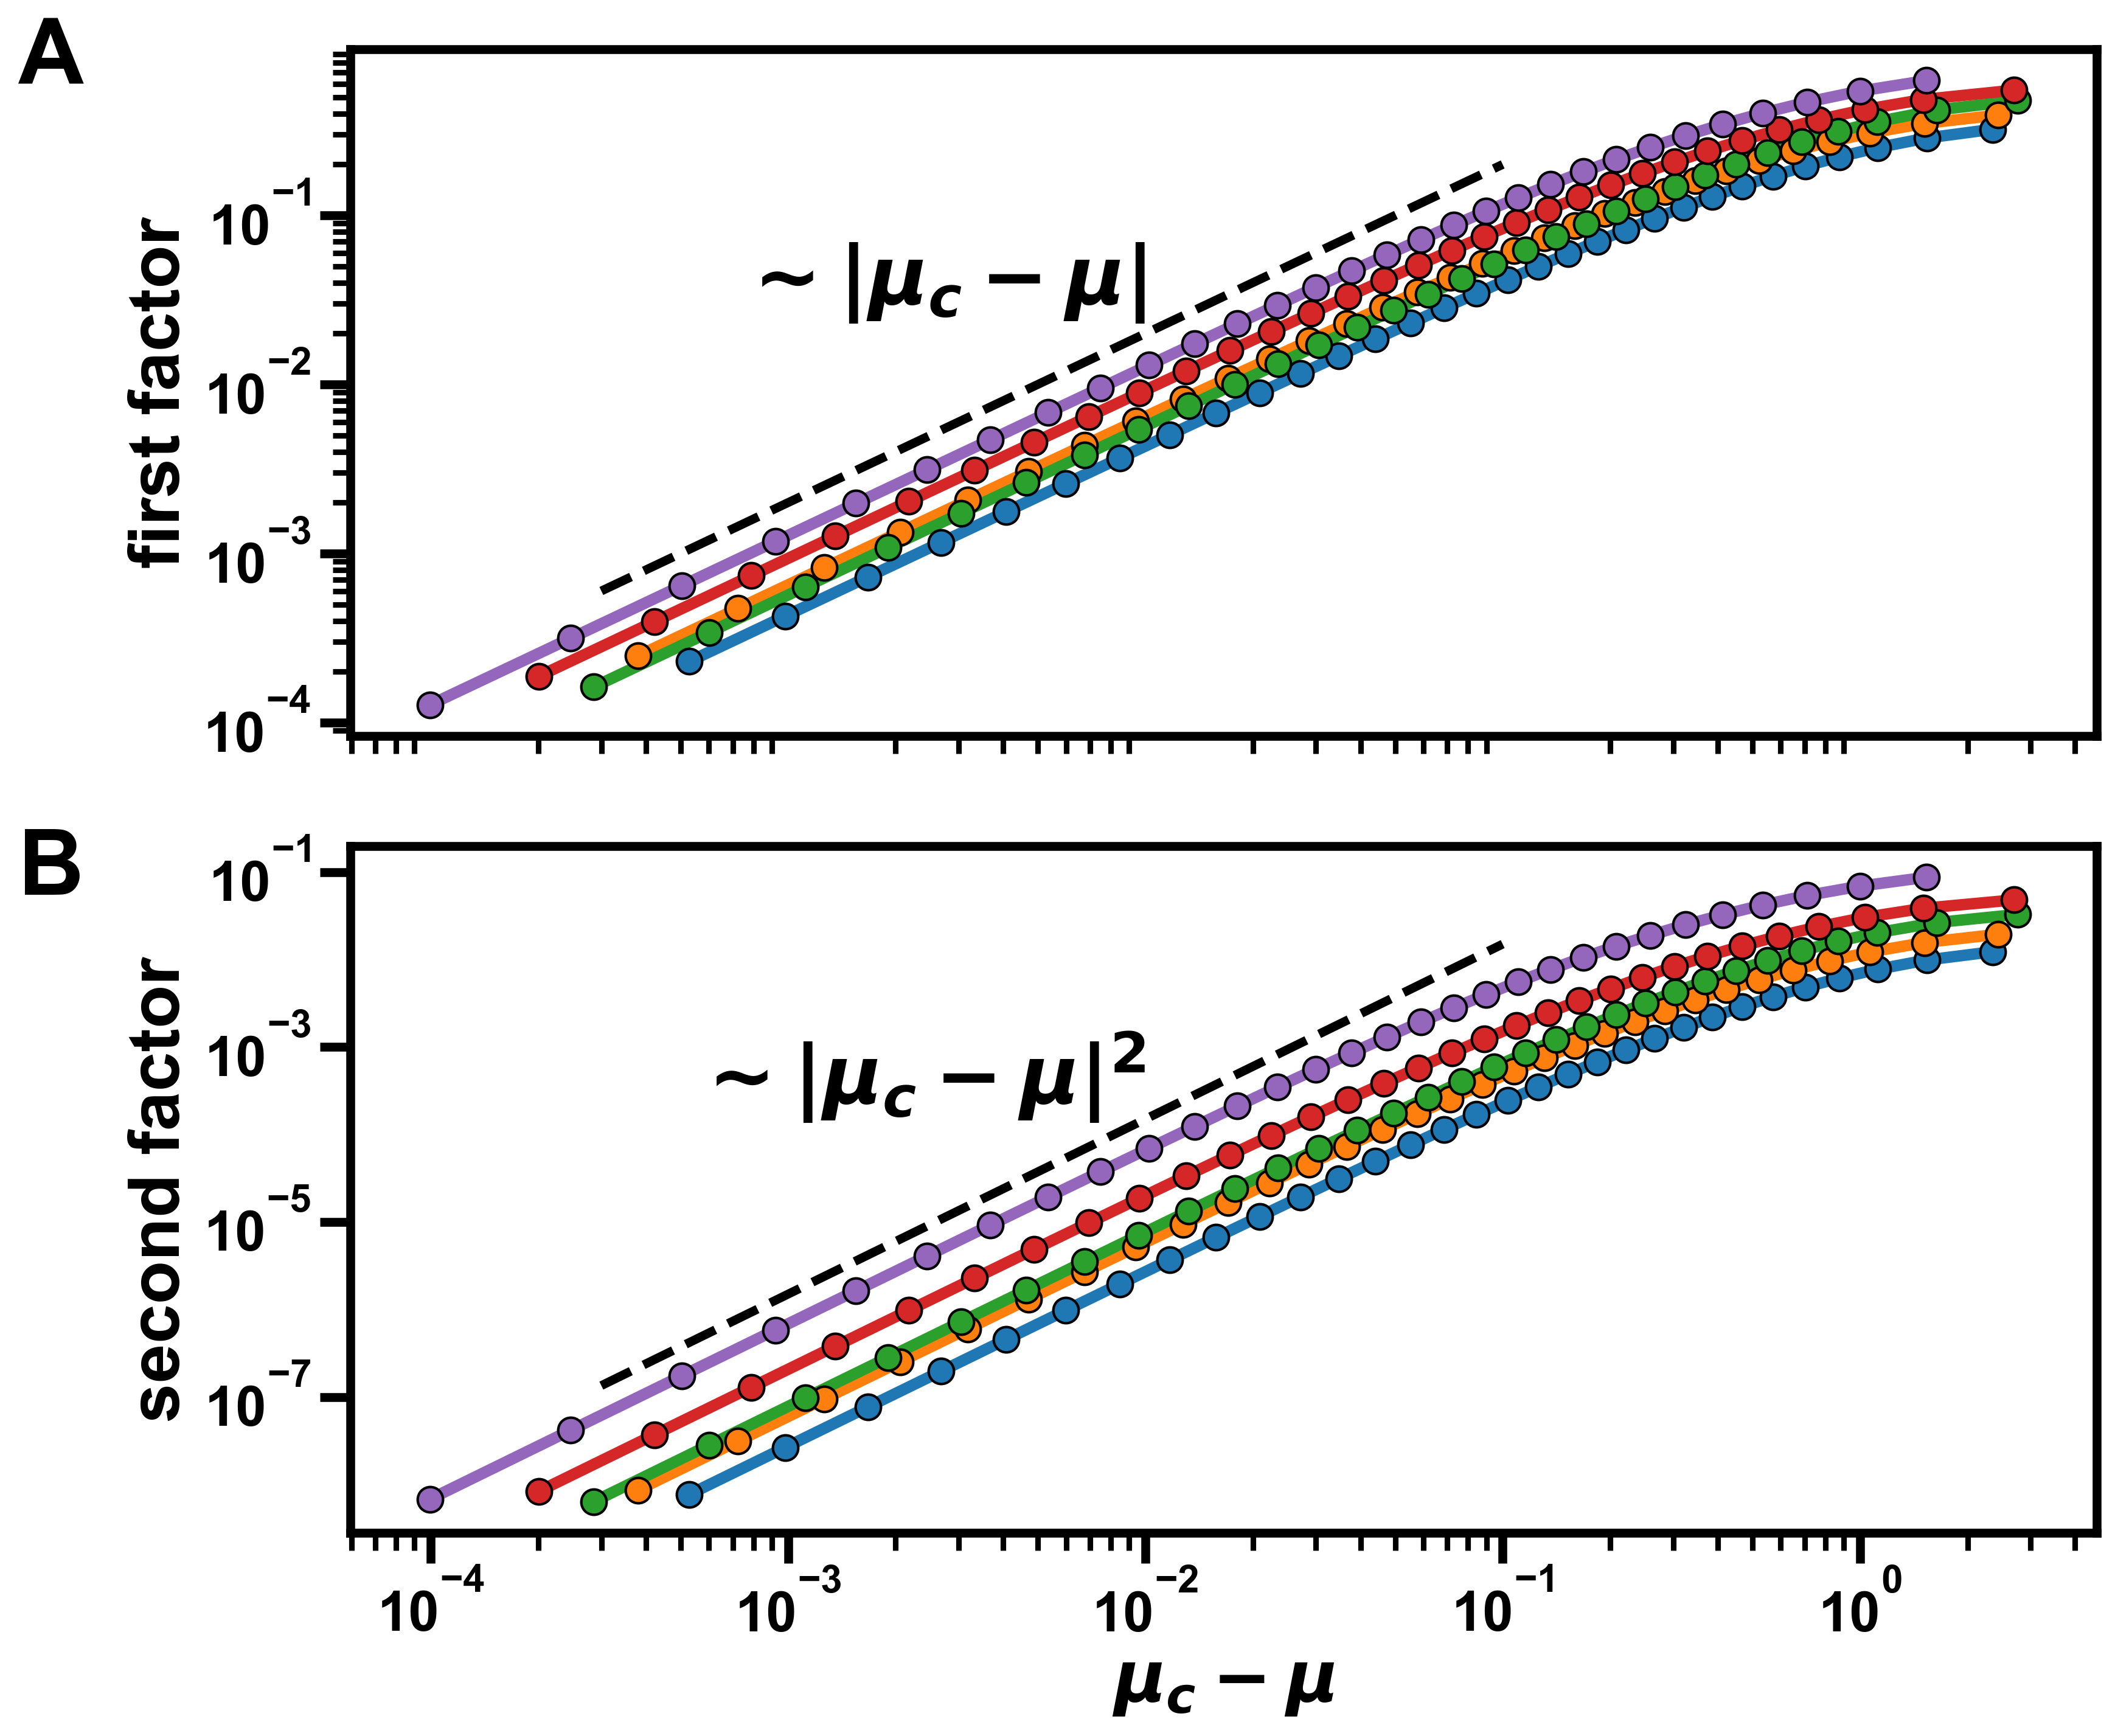
\includegraphics[width=0.95\textwidth]{figures/factor_scaling.png}
    \captionof{figure}{(A) Scaling of the quantity \(|\Delta \boldsymbol{\phi}|^2\), which is proportional to the first factor, and (B) the second factor \(|f(\bar{\boldsymbol{\phi}}) - \sum_i \mu_i \bar{\phi}_i + \Pi|\)
    in the surface-tension approximation, obtained from the numerical results (different colors) as functions of the chemical potential difference \(|\boldsymbol\mu-\boldsymbol\mu_{c}|\)
    for interaction parameters in the domain defined in Eq.~\eqref{eq:interaction_parameters}. The dashed lines indicate the expected scaling with exponents \(1\) and \(2\) respectively.\\\newline}
    \label{fig:factor_scaling}
\end{minipage}

We have therefore shown that the first factor scales as \(|\boldsymbol{\mu}_c - \boldsymbol{\mu}|\), while the second factor scales as \(|\boldsymbol{\mu}_c - \boldsymbol{\mu}|^2\). Combining these results, we conclude that near the critical point the surface tension obeys
\[
    \gamma \;\propto\; |\boldsymbol{\mu}_c - \boldsymbol{\mu}|^{3/2} .
\]


The same scaling analysis also yields the scaling of the interfacial width:
\begin{equation}
    w 
    = \frac{\sqrt{\Delta \phi_i \,\tilde\kappa_{ij}\,\Delta \phi_j}}
           {\sqrt{ \phi_i'(0) \,\tilde\kappa_{ij}\,\phi_j'(0)}}
    \;\propto\; |\boldsymbol{\mu}_c - \boldsymbol{\mu}|^{-1/2} .
    \label{eq:width_scaling}
\end{equation}
which diverges at the critical point, as expected.

Taken together, these results provide a direct connection between the bulk
thermodynamic quantities introduced earlier in this thesis and the interfacial
properties analyzed here. The critical exponent of the surface tension, \(\gamma \sim |\boldsymbol{\mu}_c-\boldsymbol{\mu}|^{3/2}\), is consistent
with the numerically obtained exponent.
In this sense, the effective interfacial model does not introduce new critical behavior, but rather,
it implies that near the critical point the interfacial properties depend more strongly on the bulk compositions than on the detailed profile shape.

\subsubsection{Sources of error and limitations}

The piecewise-linear approximation differs from the true equilibrium interfacial
profiles in two essential ways: First, it replaces the smooth, nonlinear variation
of the volume fractions across the interface by a linear interpolation. Second, it
assumes that all species share a common interfacial window, thereby neglecting
interfacial adsorption.\\

\noindent
\begin{minipage}{0.5\textwidth}

To quantify the importance of interfacial adsorption, we fit a hyperbolic tangent
profile of the form
\[
    \begin{aligned}
    \phi_i(x)
    &=
    \frac{\Delta \phi_i}{2}\,
    \tanh\!\left(\frac{x - x_{0,i}}{w}\right)
    + \bar{\phi}\\
    & i \in \{0,1\}
    \end{aligned}
\]\\
to the numerical equilibrium profiles of components 0 and 1 for the symmetric case shown in Fig.~\ref{fig:fit_profiles}A, where \(\chi_{02}=\chi_{12}\).
A tentative measure of the degree of interfacial adsorption is the displacement between the centers of the fitted profiles of components 0 and 1, which we denote by
\[\Delta x_0 = |x_{0, 0} - x_{0,1}|.\]
The interpretation of this measure becomes clear in the limiting cases.
For \(\Delta x_0 = 0\), the profile of component 2 remains constant across the interface, indicating the absence of interfacial adsorption.
In contrast, when \(\Delta x_0 \gg w\), a third phase develops in the interfacial region, corresponding to strong interfacial adsorption.\\

The results of the fits are shown in Fig.~\ref{fig:fit_profiles}B, together with the relative error
of the surface-tension approximation. A clear correlation is observed between the
relative error and the displacement between the centers of the profiles of components 0 and 1.\\

    
\end{minipage}
\hfill
\begin{minipage}{0.45\textwidth}
    \centering
    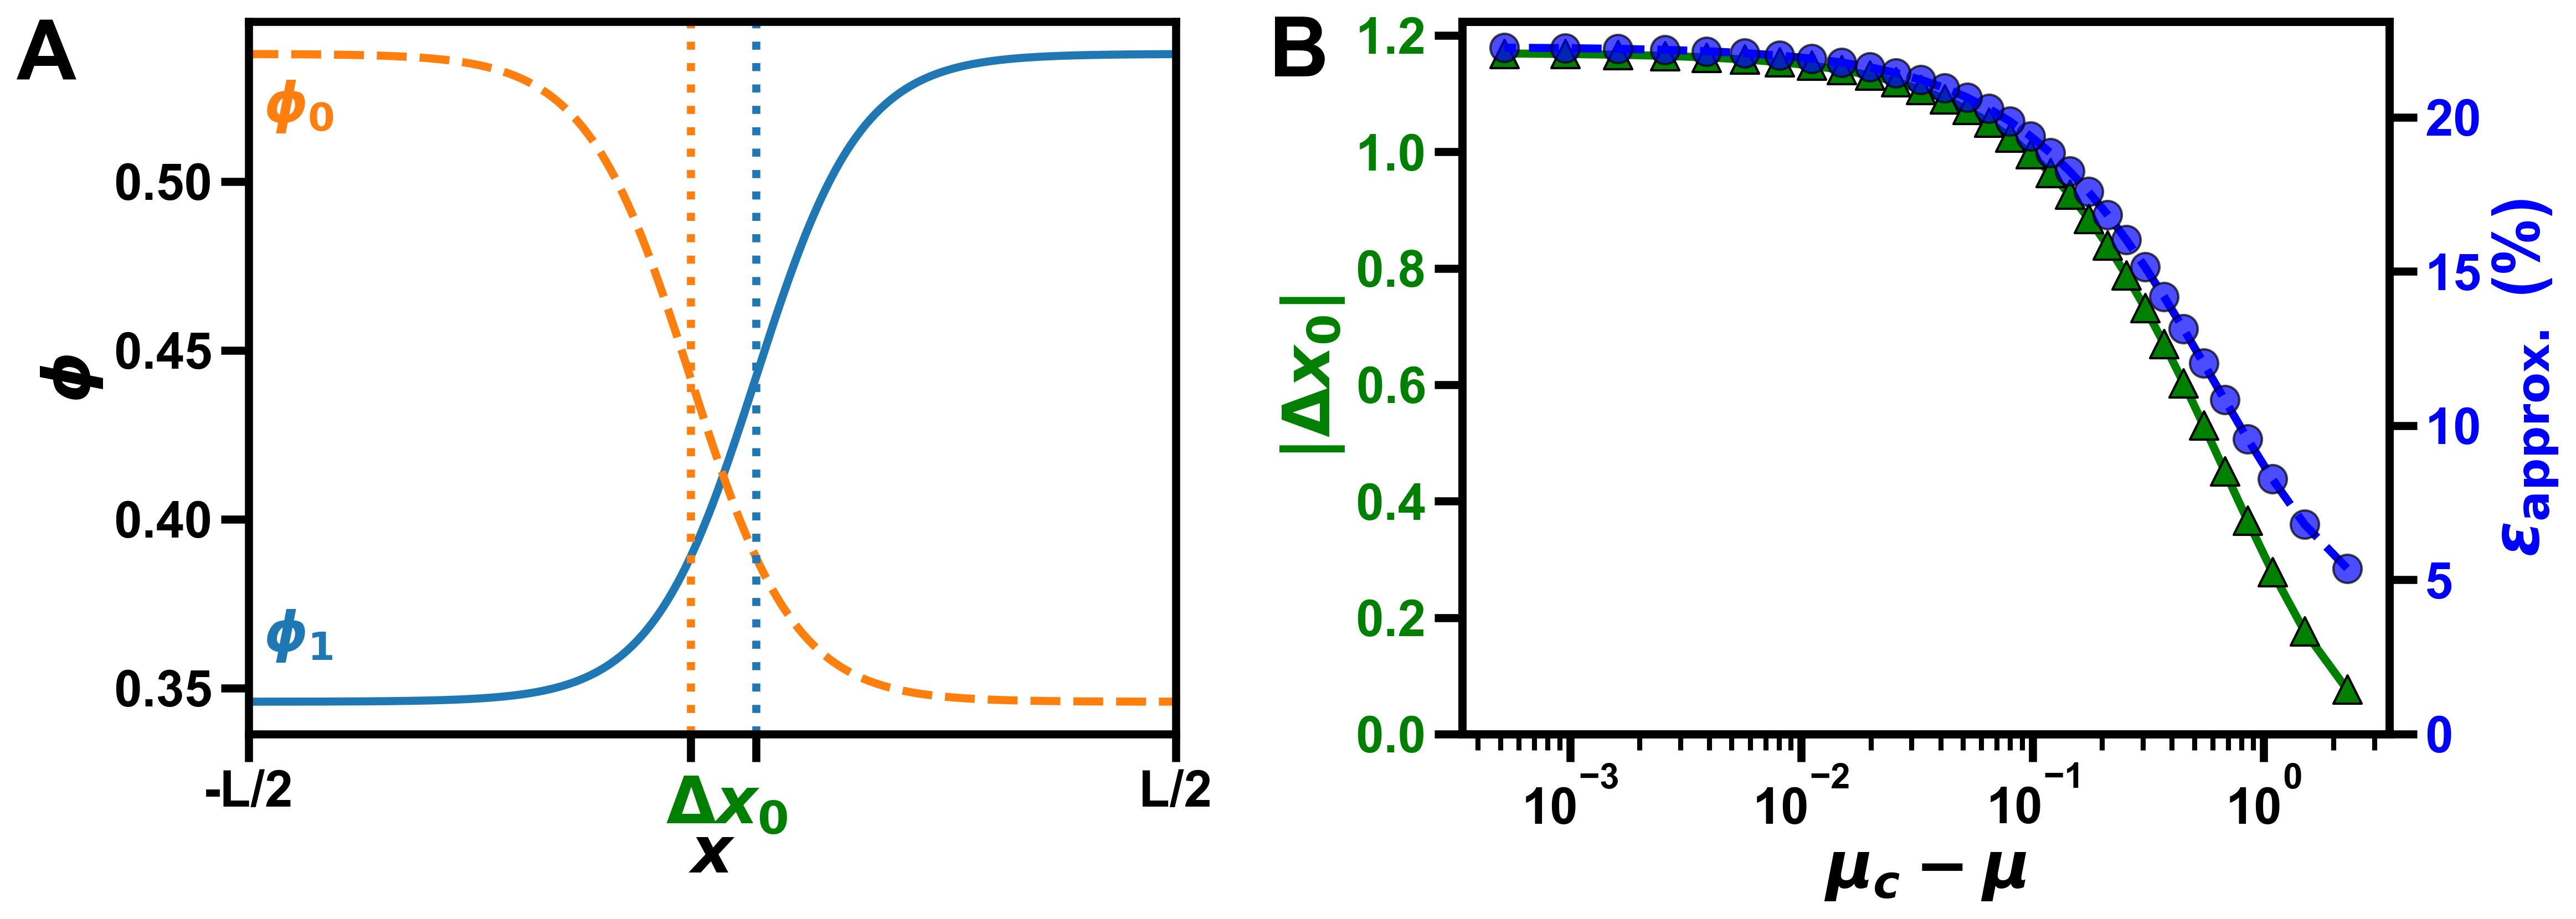
\includegraphics[width=\textwidth]{figures/fit_profiles.png}
    \captionof{figure}{(A) Hyperbolic tangent fits (solid lines) to the numerical equilibrium profiles for the symmetric case \(\chi_{02}=\chi_{12}\), used to extract the interface positions \(x_{0,i}\) (dashed vertical lines) for components 0 and 1.
    (B) Relative error of the surface-tension approximation (blue) and the displacement between the centers of the fitted profiles (green) as functions of \(|\boldsymbol\mu_c - \boldsymbol{\mu}|\).\\}
    \label{fig:fit_profiles}
    
\end{minipage}

Importantly, within the symmetric family \(\chi_{02}=\chi_{12}\), this correlation is not restricted to the specific interaction
parameters shown in Fig.~\ref{fig:fit_profiles}, but is also observed for other
interaction strengths.\\

One thing to note in Fig.~\ref{fig:fit_profiles}B is that even when the displacement between the centers of the profiles nearly vanishes in the dilute limit, the relative error stays finite.
This indicates that in the absence of interfacial adsorption, the simplified functional form of the profile still contributes to the error of the approximation. However, this baseline error (approximately \(5\%\) in Fig.~\ref{fig:fit_profiles}B) is substantially smaller than the error observed close to the critical point (approximately \(22\%\) in Fig.~\ref{fig:fit_profiles}B), where the displacement between the centers of the profiles is largest.
Therefore in conclusion, we have found that interfacial adsorption, rather than the
simplified functional form of the profile, is likely the primary limitation of the
piecewise-linear model.\\
To further analyze interfacial adsorption, we now derive analytical expressions for several interfacial properties.

\subsection{Analytical expressions for interfacial profiles in symmetric ternary mixtures}\label{sec:symmetric_case}
In this section, we consider the symmetric case, defined by \(\chi_{01}=\chi_{02}\).
In contrast to the general case, this symmetry can be exploited to derive analytical expressions for key interfacial properties.
This, in turn, provides deeper insight into the interfacial behavior and the origin of the errors in the piecewise-linear approximation.\\
The symmetric interaction matrix can be written as

\[
    \begin{pmatrix}
        0 & \chi& \eta\chi\\
         \chi& 0&  \eta\chi\\
        \eta\chi & \eta\chi& 0\\

    \end{pmatrix}
\]

where \(\chi\) denotes the interaction strength between components 0 and 1, and \(\eta\) modulates the interaction strength of component 2 with the other two species. We typically restrict attention to \(0 \le \eta \le 1\).
We adopt this notation to match earlier work \cite{Huang1996,Huang1996AnalyticInterface,Huang1999} on symmetric ternary mixtures.


\subsubsection{Implicit expression for the bulk phase compositions}
The interaction matrix of the reduced two-component system can be obtained from the original three-component interaction matrix according to Eq.~\ref{eq:reduced_chi}, which for the symmetric case reduces to\\

\[
    \begin{pmatrix}
         \chi_d & \chi_o \\
        \chi_o & \chi_d
    \end{pmatrix}
\]

where \(\chi_d = -2\eta\chi\) and \(\chi_o=\chi(1-2\eta)\) are the diagonal and off-diagonal elements, respectively. To keep the notation compact, we suppress tildes on the reduced interaction and gradient coefficients throughout this subsection.
Setting the lattice size to \(a = 1\), the reduced gradient coefficients satisfy \(\kappa_{ij} = -\chi_{ij}\).
The profiles are then determined by the variational principle \(\delta F/\delta \phi_i = \mu_i\), which for the Flory-Huggins free-energy in Eq.~\eqref{eq:fh_free_energy} leads to the following Euler-Lagrange equations:
\[
\begin{aligned}
    &-\chi_d \phi_0''(x) - \chi_o \phi_1''(x) = \chi_d \phi_0 + \chi_o \phi_1 + \ln(\phi_0) - \ln(1-\phi_0-\phi_1)-\mu_0\\
    &-\chi_o \phi_0''(x) - \chi_d  \phi_1''(x) = \chi_o \phi_0 + \chi_d \phi_1 + \ln(\phi_0) - \ln(1-\phi_0-\phi_1)-\mu_1\\
\end{aligned}
\]
Here \(\mu_0=\mu_1=\mu=\chi_d\phi_0^{(1)} + \chi_o \phi_1^{(1)} + \ln(\phi_0^{(1)}) - \ln(\phi_2^{(1)})\) is the exchange chemical potential.
Because the reduced interaction matrix is symmetric, it is natural to diagonalize the problem by introducing the eigenmodes \(\phi_\pm = \frac{1}{2}(\phi_0 \pm \phi_1)\). The Euler-Lagrange equations then become
\begin{equation}
\begin{aligned}
    &\frac{2}{\phi_s} \phi_+''(x) = -\frac{2}{\phi_s}\phi_+(x) + \ln(\phi_+ + \phi_-) + \ln(\phi_+ - \phi_-) - 2 \ln(1-2\phi_+) - 2\mu \\
    &\frac{2}{\phi_c} \phi_-''(x) = -\frac{2}{\phi_c}\phi_-(x) + \ln(\phi_+ + \phi_-) - \ln(\phi_+ - \phi_-)\\
\end{aligned}
\label{eq:el_symmetric}
\end{equation}
where the first line is obtained by adding the two original equations, while the second line follows from subtracting them. Here, the parameters \(\phi_c\) and \(\phi_s\) are defined by \(\chi_o - \chi_d \eqcolon 1/\phi_c\) and \(\chi_o + \chi_d \eqcolon -1/\phi_s\).\\


To determine the coexisting bulk compositions, we first analyze the Euler-Lagrange equation for \(\phi_-\) in the bulk. In this regime, gradient terms vanish and the fields approach the constants \(\phi_+(x\rightarrow \infty) = \bar\phi\) and \(\phi_-(x\rightarrow \infty) = \Delta \phi\).
Here \(\Delta \phi = (\phi_0^{(1)}-\phi_1^{(1)})/2\) is half the difference between the bulk phases and \(\bar\phi = (\phi_0^{(1)}+\phi_1^{(1)})/2\) is their mean composition.
The EL equation for \(\phi_-\) then reduces to
\begin{equation}
\begin{aligned}
    &-\frac{2}{\phi_c}\Delta \phi + \ln(\bar\phi + \Delta\phi)-\ln(\bar\phi - \Delta\phi) = 0\\
    \Rightarrow\quad&\Delta \phi = \bar\phi\tanh\left(\frac{\Delta\phi}{\phi_c}\right)\\
\end{aligned}
\label{eq:delta_phi}
\end{equation}
Thus, Eq.~\eqref{eq:delta_phi} provides an implicit relation between the phase-composition difference \(\Delta\phi\) and the mean composition \(\bar\phi\). To understand its solution structure, we rewrite it as
\[
x = b \tanh(x),
\]
where $x\coloneq\Delta \phi / \phi_c$ and $b\coloneq\bar\phi/\phi_c$.
This form shows immediately that if \(b\leq 1\), or equivalently \(\bar\phi \leq \phi_c\), the only root is \(x^*=0\). Hence phase separation is only possible for $\bar\phi > \phi_c$. For \(\bar\phi>\phi_c\), the positive root \(x^*>0\) satisfying \(x-b\tanh(x)=0\) increases monotonically with \(b\), so \(\Delta \phi\) also increases with \(\bar\phi\). The maximal value of \(\Delta \phi\) is reached in the binary-mixture limit \(\phi_0 \to 0\), where \(\bar\phi = 1/2\), and is determined implicitly by
\[
\Delta \phi_\mathrm{max} = \frac{1}{2}\tanh\left(\frac{\Delta\phi_\mathrm{max}}{\phi_c}\right).
\]

\subsubsection{Implicit expression for the interfacial-excess amplitude}
We now derive an implicit equation for the interfacial-excess amplitude
\[
\delta\phi_+ = \phi_+(0) - \bar\phi,
\]
which measures the peak height of the excess profile at the interface center. By contrast, the total interfacial adsorption would be obtained by integrating the excess profile across the interface.
To obtain \(\delta\phi_+\), we evaluate the Euler-Lagrange equation for \(\phi_+\) at the interface. Because \(\phi_-\) is antisymmetric about the interface, we have \(\phi_-(0)=0\), and the equation reduces to

\[
\begin{aligned}
    &\frac{2}{\phi_s} \phi_+''(0) = -\frac{2}{\phi_s}\phi_+(0) + 2\ln(\phi_+(0)) - 2 \ln(1-2\phi_+(0)) - 2\mu \\
    \Rightarrow\quad&\frac{ \phi_+''(0)}{\phi_s} = -\frac{\delta\phi_+}{\phi_s} + \frac{\Delta\phi}{\phi_c} + \ln\left(\frac{\bar\phi+\delta\phi_+}{\bar\phi+\Delta\phi}\right)+\ln\left(\frac{1-2\bar\phi}{1-2(\bar\phi+\delta\phi_+)}\right) \\
\end{aligned}
\]

where in the second line we have inserted the definition of \(\mu\)
\[
\mu = \chi_d\phi_0^{(1)} + \chi_o \phi_1^{(1)} + \ln(\phi_0^{(1)}) - \ln(\phi_2^{(1)}) = -\frac{1}{\phi_s}\bar\phi + \ln(\bar\phi+\Delta\phi) -  \ln(1-2\bar\phi).
\]
Rearranging this relation yields the implicit equation
\begin{equation}
    \delta \phi_+ =\frac{1-2\bar\phi}{2}\left(1- \frac{1}{1-2\bar\phi+2(\bar\phi+\Delta\phi)\Xi}\right).
    \label{eq:delta_phi_plus}
\end{equation}
    % \delta \phi_+ = \frac{1-2\bar\phi}{2}\frac{-2\bar\phi+2(\bar\phi+\Delta\phi)\Pi}{1-2\bar\phi+2(\bar\phi+\Delta\phi)\Pi}=\frac{1-2\bar\phi}{2}\left(1- \frac{1}{1-2\bar\phi+2(\bar\phi+\Delta\phi)\Pi}\right)
To write the result compactly, we introduce the shorthand
\begin{equation}
    \Xi = \exp\left(\frac{\delta \phi_+}{\phi_s}(1+a_2) - \frac{\Delta \phi}{\phi_c}\right)
\end{equation}
where \(a_2 = \phi_+''(0)/\delta\phi_+\) measures the curvature of \(\phi_+\) at the interface relative to the excess amplitude.
In principle, one would need another equation to determine \(a_2\) in order to solve Eq.~\eqref{eq:delta_phi_plus} self-consistently.
However, we will find that the curvature term can be neglected in the vicinity of the critical point.

To assess the importance of the curvature term, we use the scaling estimate
\[
\phi_+''(0) \sim \frac{\delta\phi_+}{w^2} 
\]
where \(w\) is the interfacial width.
This implies
\[
a_2 = \frac{\phi_+''(0)}{\delta\phi_+} \sim \frac{1}{w^2}
\]
and therefore \(a_2\) vanishes as the critical point is approached, where the interfacial width diverges. Under the assumption $|a_2| \ll 1$, Eq.~\eqref{eq:delta_phi_plus} can then be solved self-consistently once \(\Delta \phi\) is obtained from Eq.~\eqref{eq:delta_phi}. Solving these two equations yields the analytical predictions shown in Fig.~\ref{fig:absorption}.\\

\begin{minipage}{\textwidth}
    \centering
    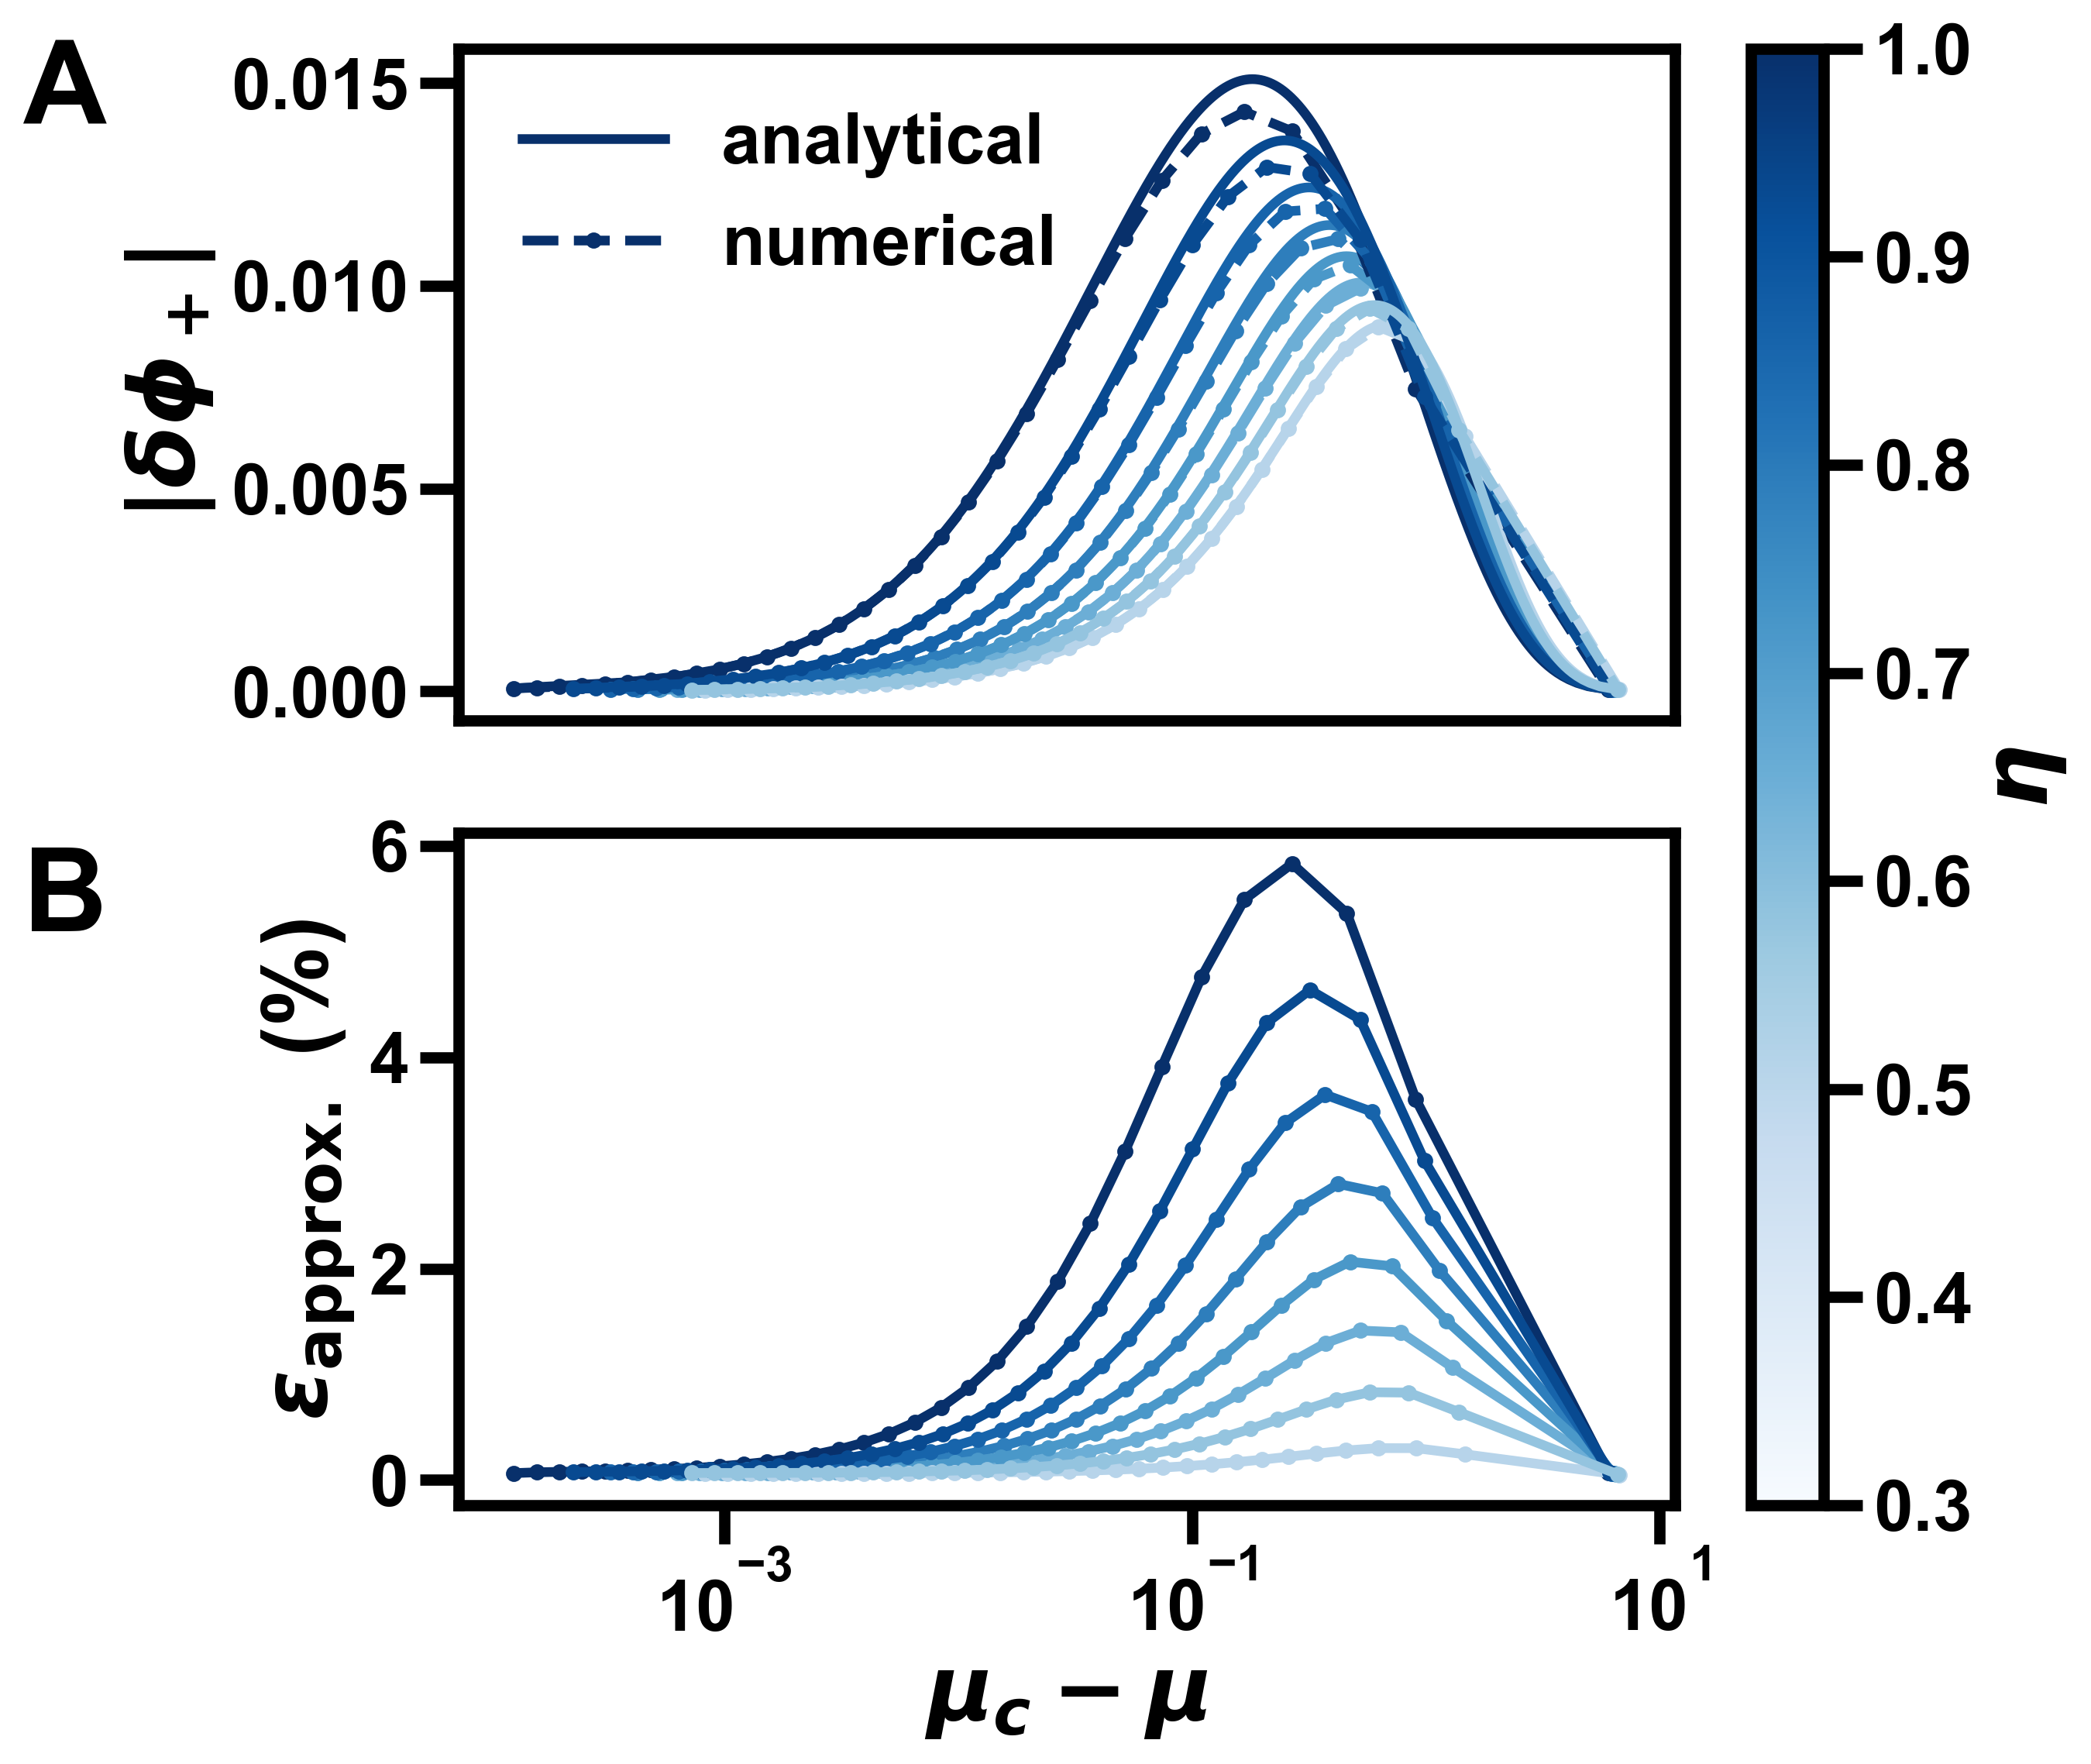
\includegraphics[width=0.8\textwidth]{figures/absorption.png}
    \captionof{figure}{(A) Interfacial-excess amplitude \(|\delta \phi_+| = |\phi_+(0) - \bar\phi|\) as a function of the chemical-potential difference \(\mu_c-\mu\).
    Dashed curves show the numerical results, while solid curves show the solution of the implicit relation, Eq.~\eqref{eq:delta_phi_plus}.
    With \(\chi=2.5\), the color scale represents the interaction strength \(\eta\). 
    The analytical solution systematically overestimates \(|\delta \phi_+|\).
    (B) Relative error \(\epsilon_{\mathrm{approx.}} = |\delta \phi_+^{\mathrm{analytical}} - \delta \phi_+^{\mathrm{numerical}}| / |\delta \phi_+^{\mathrm{numerical}}|\) of the analytical approximation.
    The error vanishes near the critical point, where the analytical solution becomes exact.
    It also appears to vanish near the binary-mixture limit \((\phi_0 \to 0)\), suggesting that curvature effects can be neglected in this regime as well.\\}

    \label{fig:absorption}
    
\end{minipage}

\subsubsection{Approximation for the interfacial profiles}\label{sss:profile_approximation}
We next derive the interfacial width \(w = \Delta \phi / \phi_-'(0)\), which extends the earlier approximation in Eq.~\eqref{eq:interface_width_approximation} by including adsorption effects. To compute \(w\), we evaluate the conserved quantity in Eq.~\eqref{eq:invariant_quantity} at the interface.
At the interface, we have \(\phi_-(0)=0\) and, by symmetry of \(\phi_+\), also \(\phi_+'(0)=0\).
% At the interface we have \(\phi_-(0) = \phi_+'(0) = 0\).
% The free-energy density at the interface is then given by
% \[
% f=2\phi_+(0)\ln(\phi_+(0))+(1-2\phi_+(0))\ln(1-2\phi_+(0))-\frac{\phi_+(0)^2}{\phi_s} + \frac{(\phi_-'(0))^2}{\phi_c} 
% \]
% The chemical potential can be rewritten in terms of the mean volume fraction \(\bar\phi=(\phi_1^{(1)}+\phi_2^{(1)})/2\) and the difference 
% \(\Delta\phi = (\phi_1^{(1)}-\phi_2^{(1)})/2\)
% \[\mu=-\bar\phi/\phi_s - \Delta\phi/\phi_c+\ln(\bar\phi+\Delta\phi)-\ln(1-2\bar\phi)\]

% and the pressure can be rewritten as
% \[
% \begin{aligned}
% \Pi = \mu 2\bar\phi - f &= -\bar\phi/\phi_s - \Delta\phi/\phi_c+\ln(\bar\phi+\Delta\phi)-\ln(1-2\bar\phi)\\
% &-(\bar\phi+\Delta\phi)\ln(\bar\phi+\Delta\phi) -(\bar\phi-\Delta\phi)\ln(\bar\phi-\Delta\phi)\\
% &-(1-2\bar\phi)\ln(1-2\bar\phi) +\frac{\bar\phi^2}{\phi_s} +\frac{\Delta\phi^2}{\phi_c} 
% \end{aligned}
% \]
\[
\begin{aligned}
    &f_\mathrm{local}(\phi_+(0)) - \mu 2\phi_+(0) + \Pi =\frac{(\phi_-'(0))^2}{\phi_c}\\
    \Rightarrow\quad&\phi_-'(0) = \sqrt{\phi_c \left(f_\mathrm{local}(\phi_+(0)) - \mu 2\phi_+(0) + \Pi\right)}\\
\end{aligned}
\]
Here \(f_\mathrm{local}\) is the local free-energy density evaluated at the interface and \(\Pi\) is the osmotic pressure. The interfacial width therefore becomes
\begin{equation}
    w = \frac{\Delta \phi}{\sqrt{\phi_c \left(f_\mathrm{local}(\phi_+(0)) - \mu 2\phi_+(0) + \Pi\right)}}
\end{equation}


\noindent
\begin{minipage}{0.5\textwidth}
Using the resulting expressions for \(\Delta \phi\), \(\delta \phi_+\), and \(w\), we propose the following approximate interfacial profiles as\\

\begin{equation}
    \begin{aligned}
        \phi_-(x) & = \Delta \phi \tanh\left(\frac{x}{w}\right),\\
        \phi_+(x) & = \bar\phi + \delta\phi_+ \sech^2\left(\frac{x}{w}\right)
    \end{aligned}
\end{equation}

For \(\phi_-(x)\), we use a hyperbolic tangent profile, since it is antisymmetric and saturates in the bulk. For the excess part of \(\phi_+(x)\), i.e. \(\phi_+(x)-\bar\phi\), we use a \(\sech^2\) form.
This profile is symmetric and has a peak at the interface.

As shown in Fig.~\ref{fig:symm_profile_approx}, the approximation matches the numerical profiles quite well, especially for \(\phi_-\). Although \(w\) is derived from \(\phi_-\), it also appears to capture the width of \(\phi_+\) accurately, suggesting that a single width is sufficient for both modes.

\end{minipage}
\hfill
\begin{minipage}{0.46\textwidth}
    \centering
    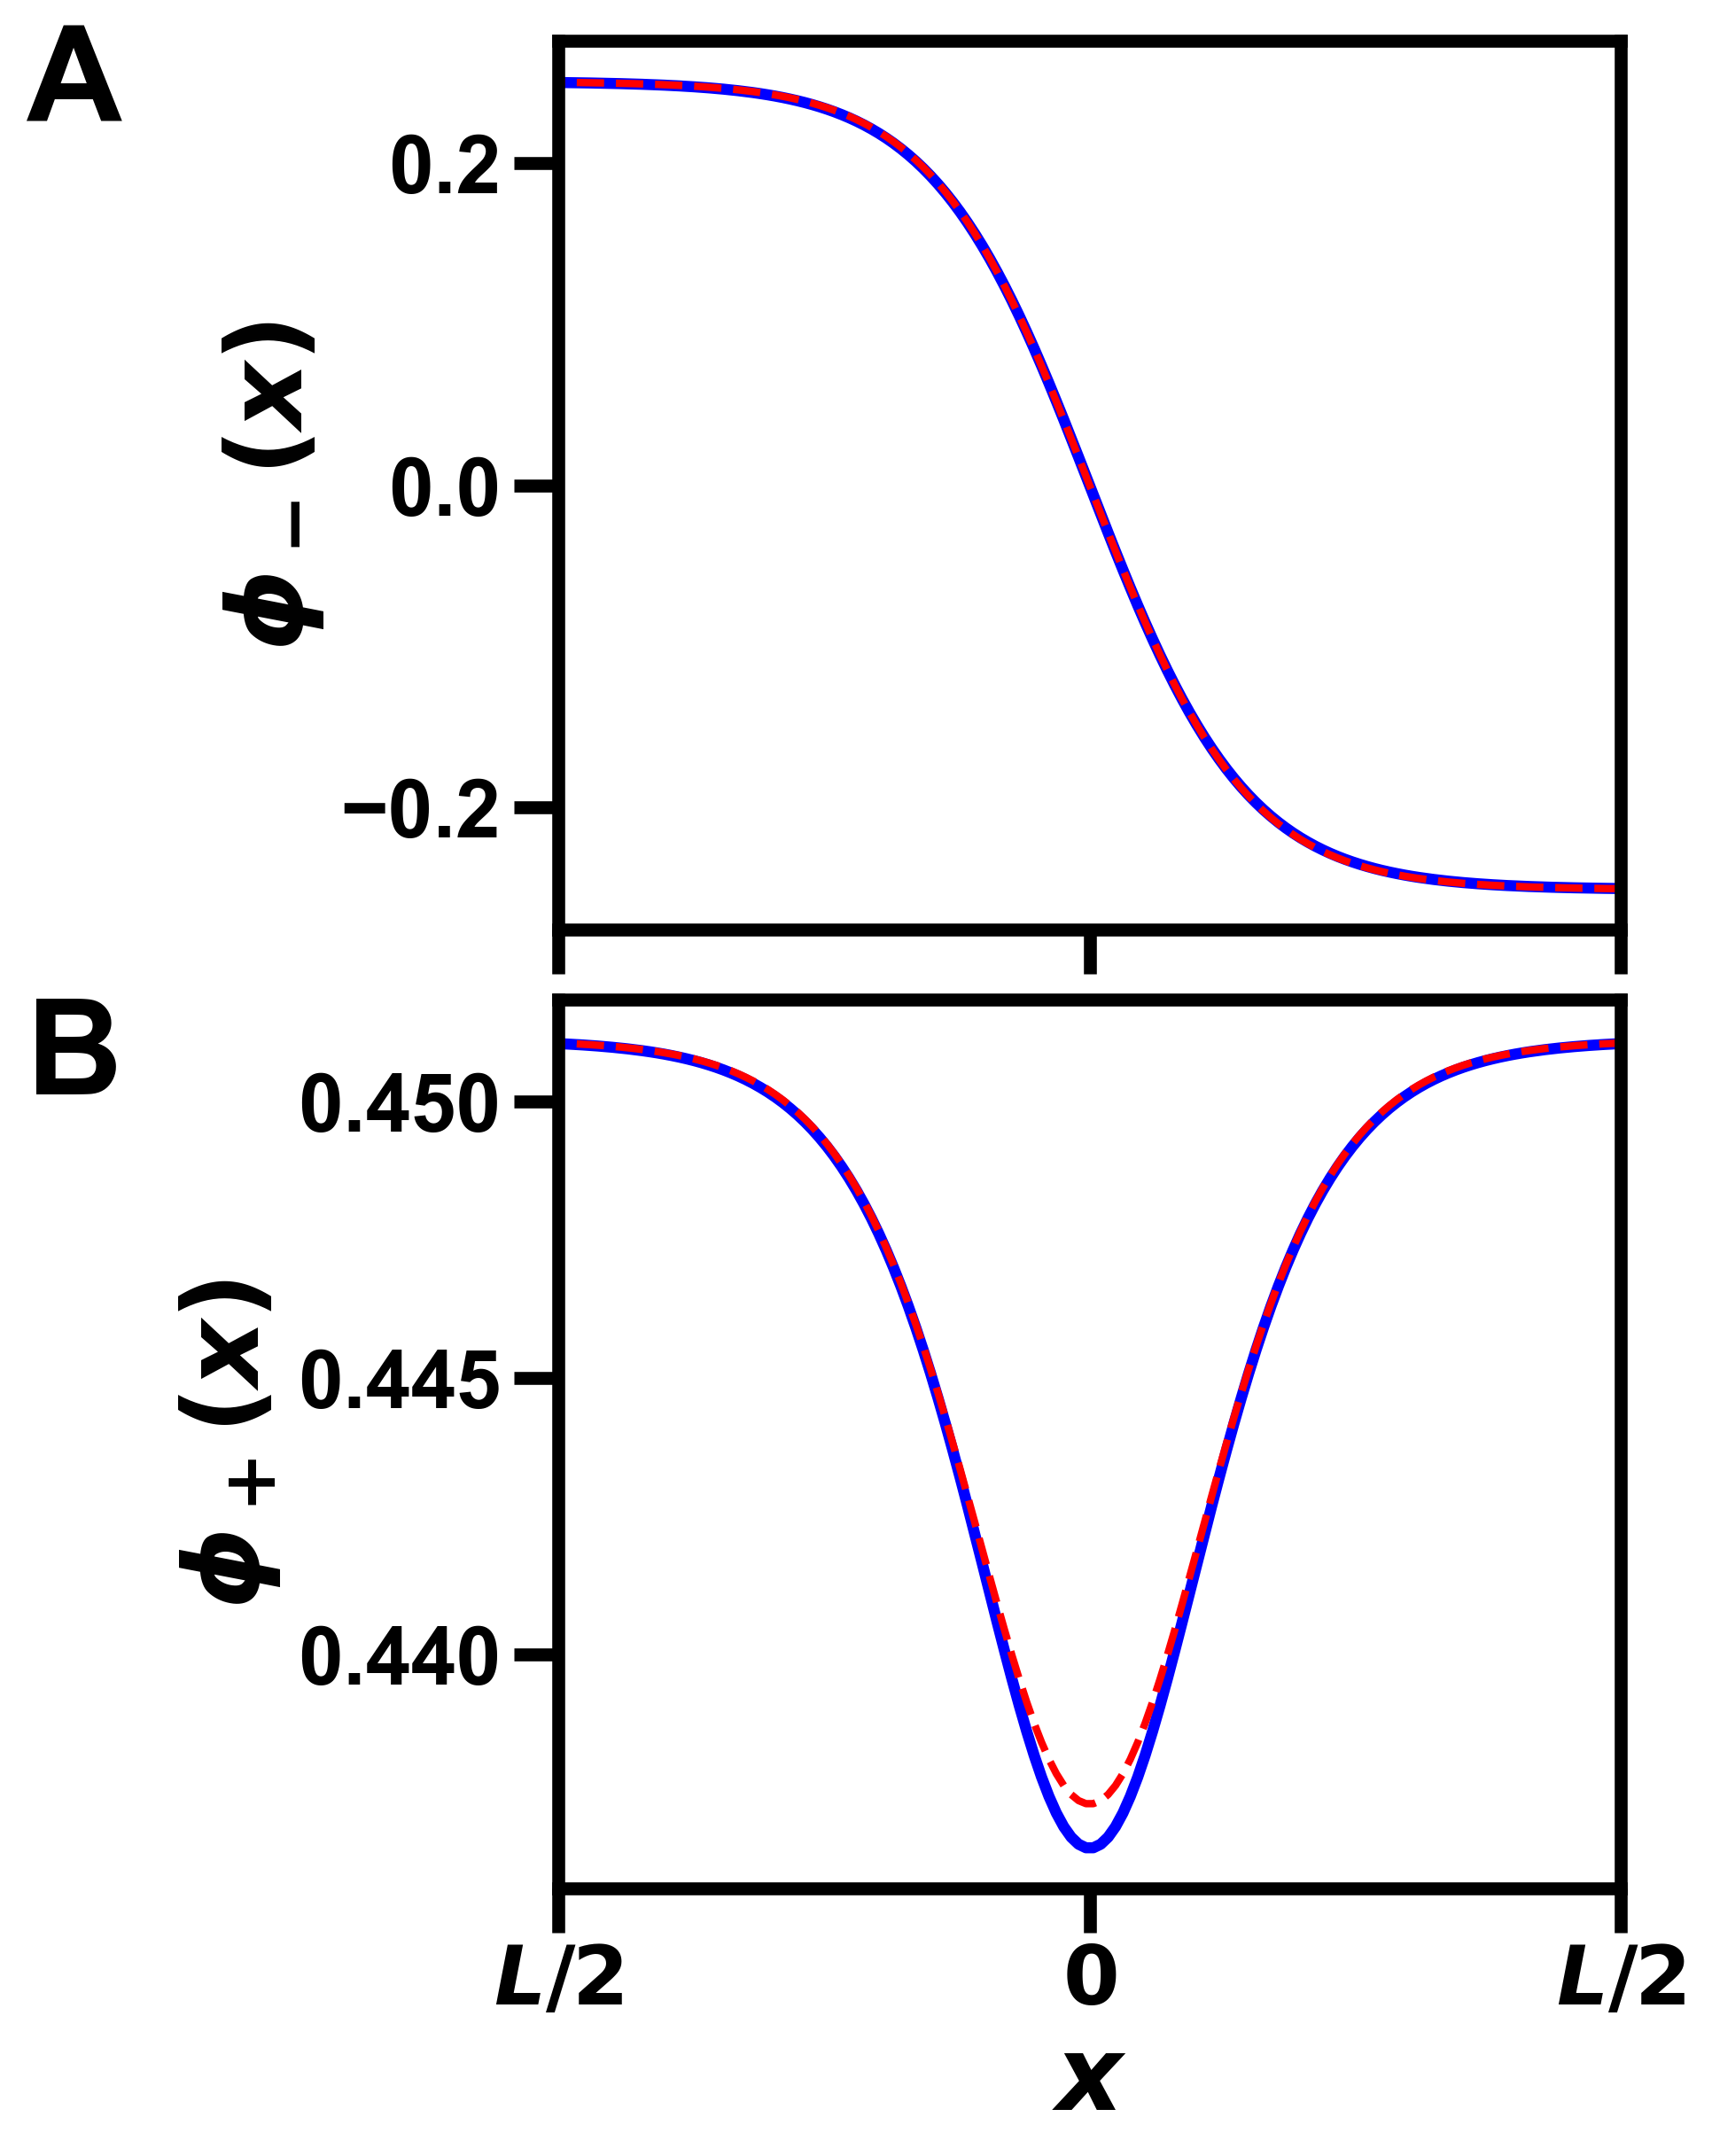
\includegraphics[width=0.95\textwidth]{figures/symm_profile_approx.png}
    \captionof{figure}{Comparison of the numerical equilibrium profiles (dashed red) with the analytical approximation (solid blue) for the symmetric ternary system: \(\phi_-(x)\) in (A)
    and \(\phi_+(x)\) (B) for \(\chi=2.5\) and \(\eta=1.0\).\\}
    \label{fig:symm_profile_approx}
 
\end{minipage}


\subsubsection{Improving the surface tension approximation}
Finally we can use the analytical expressions for the interfacial properties to improve the surface tension approximation.
The surface tension approximation in Eq.~\eqref{eq:surface_tension_approximation} can be rewritten as
\[
\gamma \approx \sqrt{(\Delta \phi_i\kappa_{ij} \Delta \phi_j)\,(f(\bar\phi+\delta\phi_+) -2\mu_i( \bar{\phi} + \delta\phi_+)+ \Pi)}
\]
Where now instead of using the mean composition \(\bar\phi\) we use the composition at the interface \(\bar\phi + \delta\phi_+\) including the effect of interfacial adsorption.
The results of this improved approximation can be seen in Fig.~\ref{fig:st_symmetric_approx}.\\

\begin{minipage}{0.95\textwidth}
    \centering
    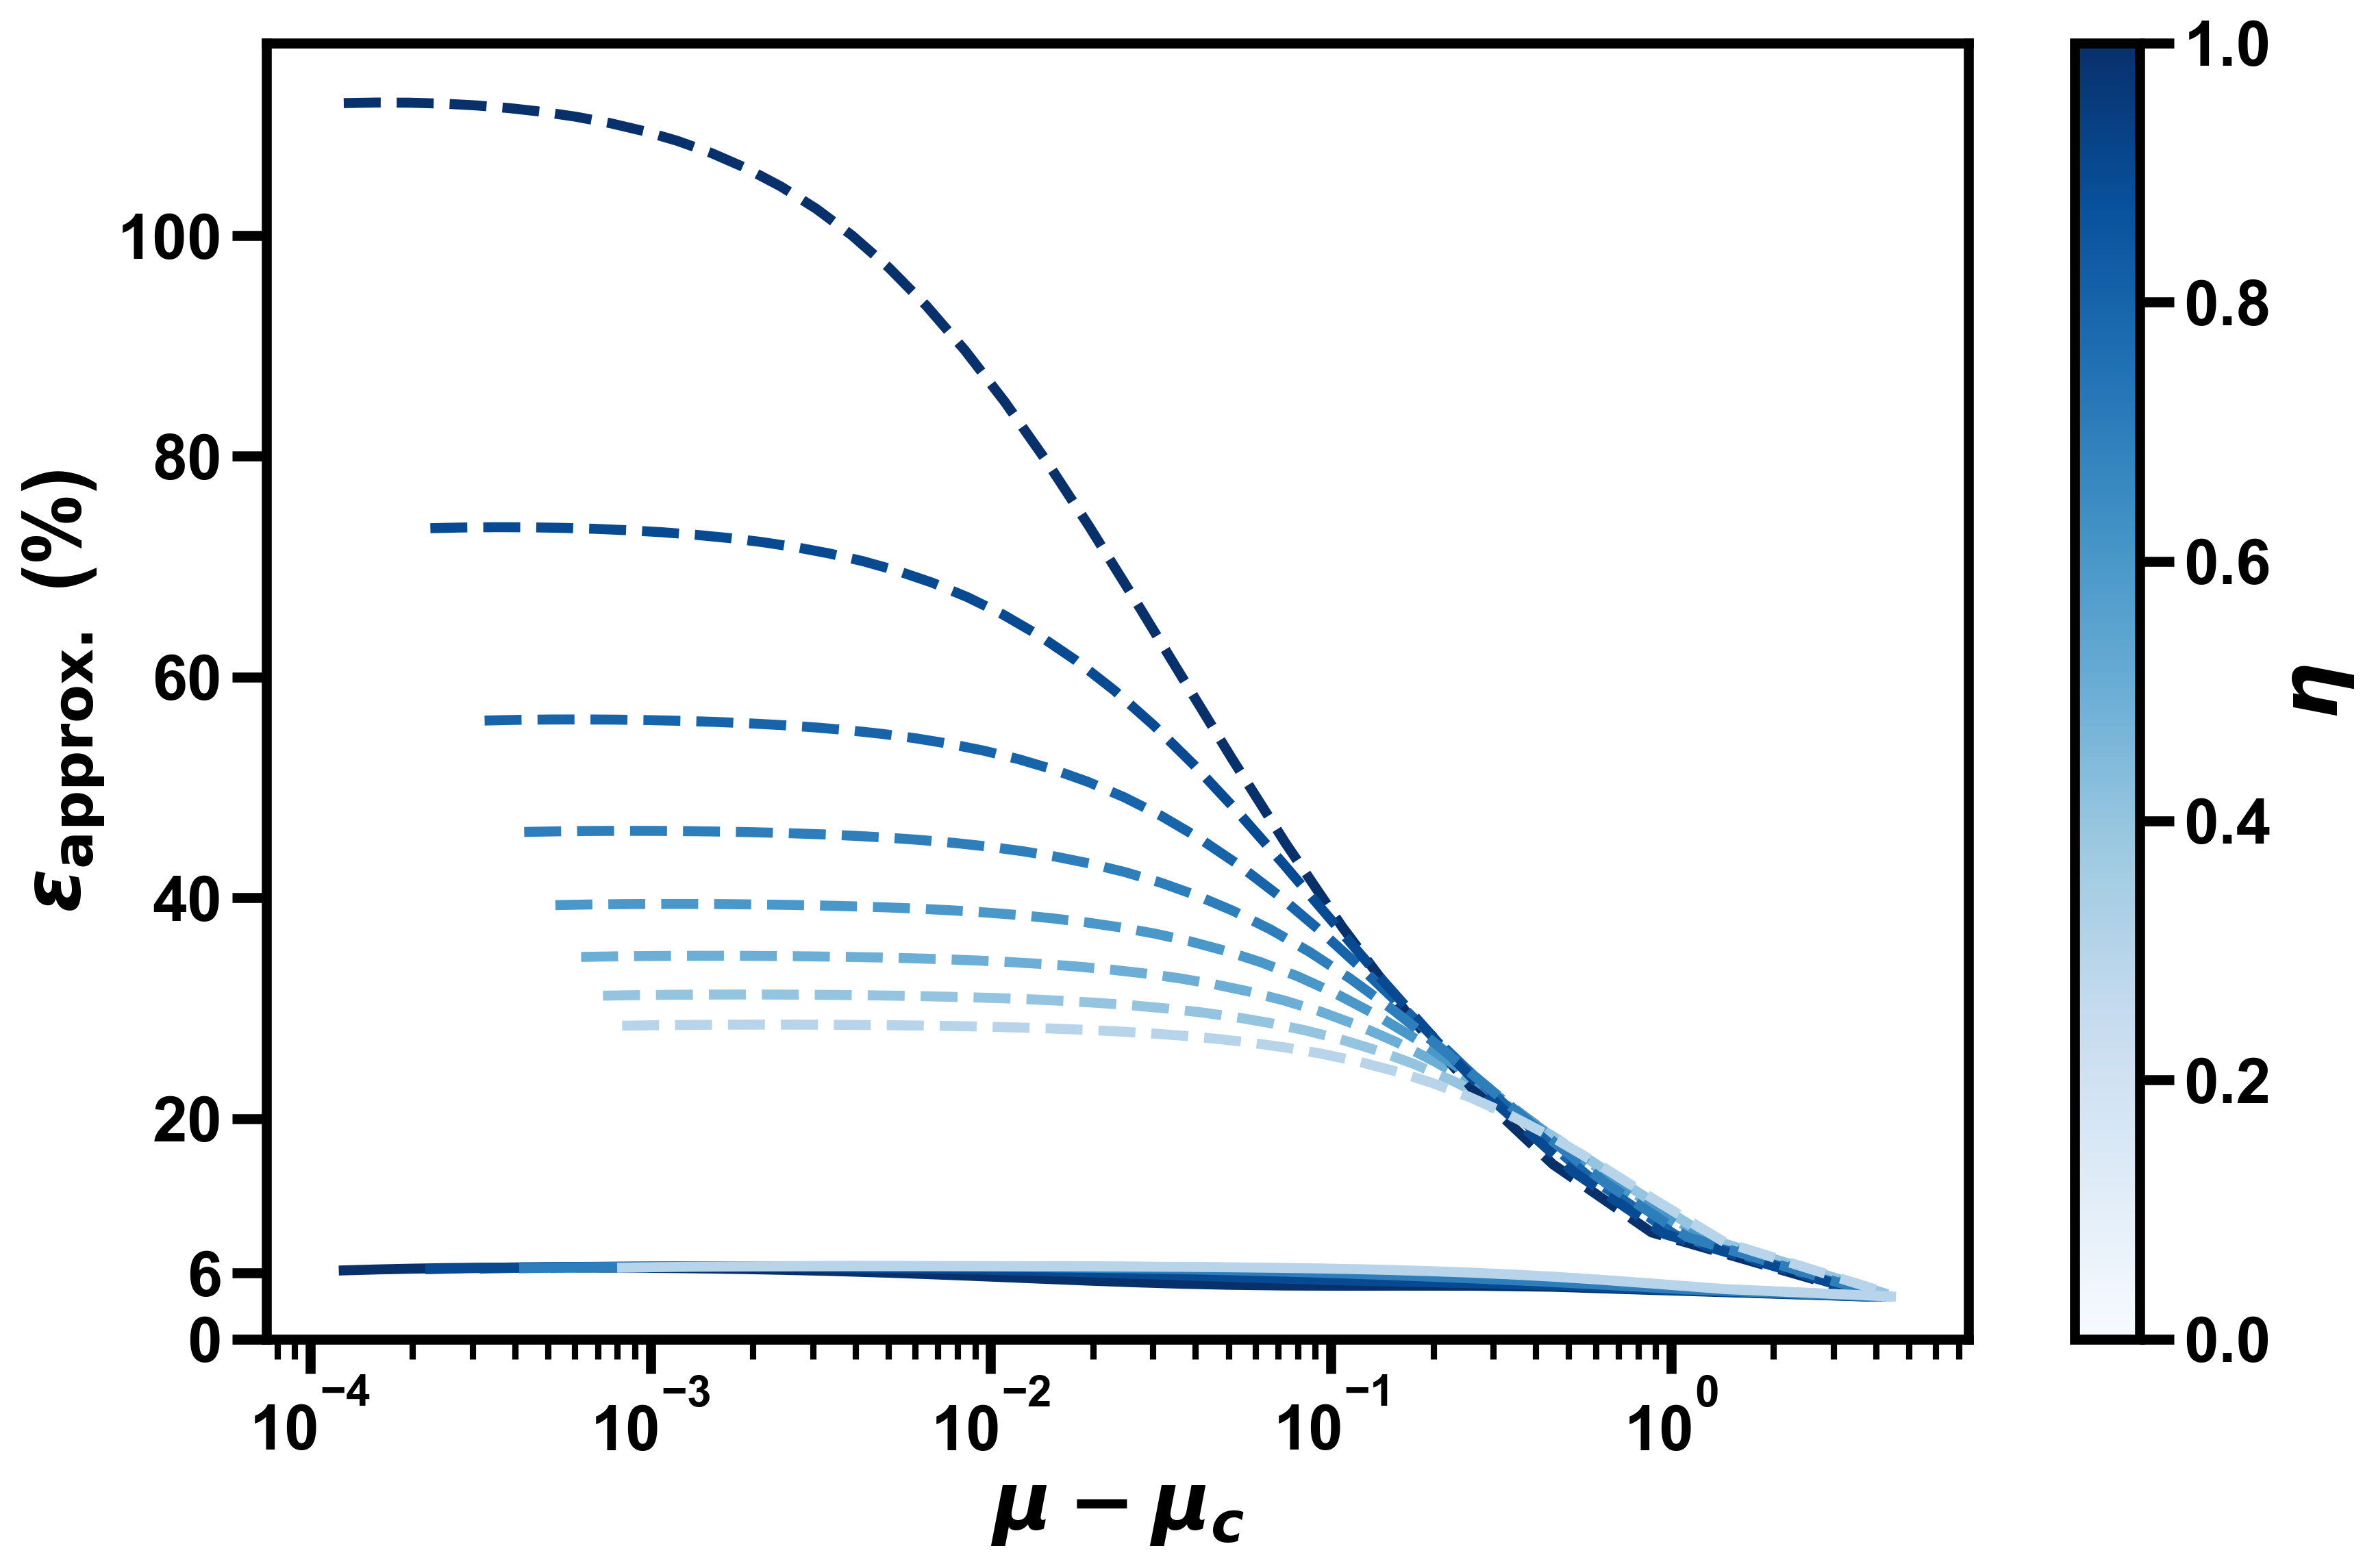
\includegraphics[width=\textwidth]{figures/st_symmetric_approx.png}
    \captionof{figure}{Relative error of the surface tension approximation for the symmetric ternary system with (solid) and without (dashed) interfacial adsorption effects included, as a function of the chemical potential difference \(\mu_c-\mu\).
    With \(\chi=2.5\), the colorscale indicates the interaction strength \(\eta\).\\}
    \label{fig:st_symmetric_approx}
\end{minipage}

Clearly, the approximation that includes interfacial adsorption effects performs much better, with a relative error of approximately \(6\%\) that remains essentially constant across phase space and all values of \(\eta\).
After accounting for interfacial adsorption, the remaining deviation from the true surface tension is likely due to the simplified functional form of the profile, which appears to contribute a baseline error for all values of \(\eta\).

\clearpage

\section{Fast Binodal Construction}\label{s:binodal_tracing}
In the previous chapter, we examined interfacial profiles in ternary systems. 
To accelerate convergence to equilibrium, the interface was initialized as a sharp step between coexisting bulk phases. 
These bulk compositions were computed using the \texttt{flory} Python package \cite{Yicheng2025flory}, which initially provided a practical solution. 
However, after optimizing the numerical scheme for the interfacial profile calculations, this precomputation became the dominant bottleneck.

Because the system was explored by stepping along the binodal, successive coexistence points are close to one another (see Fig.~\ref{fig:workflow}).
This suggests using the coexistence compositions from one step as an initial approximation for the next,
thereby accelerating convergence along the binodal.

This observation motivates the method developed in this section, which enables rapid construction of ternary binodals. 


\subsection{Tracing out the binodal curve in phase space}
To motivate the algorithm, we view the binodal geometrically in phase space. 
Each point on the binodal represents a pair of coexisting phase compositions which satisfy the coexistence conditions. 
The binodal therefore forms a lower-dimensional structure in the full phase space that can be traced continuously from one coexistence state to the next. 
This geometric viewpoint forms the basis of the continuation method developed below. The overall strategy and the special cases discussed in this section are summarized schematically in Fig.~\ref{fig:tracer_schematics}. 


\subsubsection{Coexistence conditions}

A coexistence state of two phases in a ternary system can be represented by a point in phase space,
\[
\boldsymbol\phi = (\phi_1^{(1)}, \phi_2^{(1)}, \phi_1^{(2)}, \phi_2^{(2)})^T,
\]
where the superscript labels the phase and the subscript labels the species.
These coordinates are not independent, but must satisfy the coexistence conditions introduced in Eq.~\eqref{eq:coexistence_conditions}. In particular, the two independent exchange chemical potentials and the osmotic pressure must be equal in both phases. Defining
\[
\boldsymbol{E}
=
(\mu_1^{(1)}-\mu_1^{(2)},\, \mu_2^{(1)}-\mu_2^{(2)},\, \Pi^{(1)}-\Pi^{(2)})^T,
\]
these conditions can be written compactly as
\[
\boldsymbol{E}(\boldsymbol{\phi}) = \boldsymbol{0}.
\]


For the Flory-Huggins free-energy density, the exchange chemical potentials and osmotic pressure are given by
\[
\begin{aligned}
    \mu_i(\phi_1, \phi_2) &= \frac{\partial f}{\partial \phi_i}
    = \ln(\phi_i) - \ln(\phi_0) + \sum_{j=1}^2 \tilde\chi_{ij}\phi_j,\\
    \Pi(\phi_1, \phi_2) &= -f + \sum_i \mu_i \phi_i
    = -\ln(\phi_0) + \frac{1}{2}\sum_{i,j=1}^2 \phi_i \tilde\chi_{ij} \phi_j.
\end{aligned}
\]

The algorithm described in the following sections starts from such a coexistence state \(\boldsymbol\phi\). 


\subsubsection{Tangential step along the binodal}

Suppose that a coexistence state \(\boldsymbol{\phi}\) on the binodal is known. We can then ask whether one can take a small step away from this point while remaining on the binodal.
For a sufficiently small displacement
\[
\delta\boldsymbol{\phi}_t
=
(\delta\phi_1^{(1)}, \delta\phi_2^{(1)}, \delta\phi_1^{(2)}, \delta\phi_2^{(2)})^T,
\]
linearizing the coexistence conditions gives
\begin{equation}
\boldsymbol{E}(\boldsymbol{\phi}+\delta\boldsymbol{\phi}_t)
=
\boldsymbol{E}(\boldsymbol{\phi})
+
\boldsymbol{J}\,\delta\boldsymbol{\phi}_t
+
\mathcal{O}(\delta\boldsymbol{\phi}_t^2)
=
\boldsymbol{0},
\label{eq:binodal_step}
\end{equation}
where \(\boldsymbol{J}\) is the Jacobian matrix defined as
\[
\boldsymbol{J} =
\begin{pmatrix}
\frac{\partial \mu_1^{(1)}}{\partial \phi_1^{(1)}} & \frac{\partial \mu_1^{(1)}}{\partial \phi_2^{(1)}} & -\frac{\partial \mu_1^{(2)}}{\partial \phi_1^{(2)}} & -\frac{\partial \mu_1^{(2)}}{\partial \phi_2^{(2)}}\\
\frac{\partial \mu_2^{(1)}}{\partial \phi_1^{(1)}} & \frac{\partial \mu_2^{(1)}}{\partial \phi_2^{(1)}} & -\frac{\partial \mu_2^{(2)}}{\partial \phi_1^{(2)}} & -\frac{\partial \mu_2^{(2)}}{\partial \phi_2^{(2)}}\\
\frac{\partial \Pi^{(1)}}{\partial \phi_1^{(1)}} & \frac{\partial \Pi^{(1)}}{\partial \phi_2^{(1)}} & -\frac{\partial \Pi^{(2)}}{\partial \phi_1^{(2)}} & -\frac{\partial \Pi^{(2)}}{\partial \phi_2^{(2)}}
\end{pmatrix}.
\]
where we have used the fact that the coexistence conditions involve differences of chemical potentials and osmotic pressure between the two phases, which leads to the minus signs in the last two columns of \(\boldsymbol{J}\).

Since \(\boldsymbol{\phi}\) is assumed to already lie the binodal, we have \(\boldsymbol{E}(\boldsymbol{\phi})=\boldsymbol{0}\). Remaining on the binodal to first order therefore requires
\[
\boldsymbol{J}\,\delta\boldsymbol{\phi}_t = \boldsymbol{0}.
\]
In other words, the displacement in phase space that preserves the coexistence conditions to first order is given by the null space of the Jacobian,
\[
\delta\boldsymbol{\phi}_t \in \operatorname{null}(\boldsymbol{J}).
\]
Because the Jacobian is a \(3 \times 4\) matrix, its null space is generically one-dimensional, so there is a unique local direction along which one can step.


\subsubsection{Projecting back onto the coexistence manifold}

The tangential step derived above follows the local direction of the binodal, but it is only accurate to first order.
As a result, the predicted point generally deviates from the coexistence manifold by an error of order \(\|\delta\boldsymbol{\phi}_t\|^2\).
If left uncorrected, this error accumulates over many steps and can eventually lead to a noticeable drift away from the binodal.

One way to reduce this drift is to take smaller tangential steps, but this also increases the number of iterations required to trace out the curve.
A more efficient approach is therefore to add a correction step that projects the predicted point back onto the coexistence manifold.

Suppose that \(\boldsymbol{\phi}\) is close to, but not exactly on, the binodal.
Linearizing the coexistence conditions as in Eq.~\ref{eq:binodal_step} gives
\begin{equation}
\boldsymbol{E}(\boldsymbol{\phi}+\delta\boldsymbol{\phi}_t)
=
\underbrace{\boldsymbol{E}(\boldsymbol{\phi})}_{\neq 0}
+
\boldsymbol{J}\,\delta\boldsymbol{\phi}_n
+
\mathcal{O}(\delta\boldsymbol{\phi}_n^2)
=
\boldsymbol{0},
\end{equation}
We therefore seek a correction that cancels the residual coexistence error to first order, which needs to satisfy

\[
\boldsymbol{J}\,\delta\boldsymbol{\phi}_n + \boldsymbol{E}(\boldsymbol{\phi}) = \boldsymbol{0}.
\]

Because \(\boldsymbol{J}\) has a nontrivial null space, this equation does not have a unique solution: one may always add a component along the tangent direction without changing the first-order satisfaction of the coexistence conditions. To keep the correction separate from motion along the binodal, we choose the minimum-norm solution,
\[
\delta\boldsymbol{\phi}_n = -\boldsymbol{J}^+ \boldsymbol{E}(\boldsymbol{\phi})\in \operatorname{null}(\boldsymbol{J})^\perp,
\]
where 
\[\boldsymbol{J}^+ = \boldsymbol{J^T}(\boldsymbol{J}\boldsymbol{J^T})^{-1}\]

denotes the Moore-Penrose pseudoinverse of \(\boldsymbol{J}\). This choice makes the correction step orthogonal to the null space of \(\boldsymbol{J}\), so that it does not introduce any additional motion along the binodal. In this way, the tangential step and the projection step remain cleanly separated.

In practice, we compute the pseudoinverse using the singular value decomposition
\[
\boldsymbol{J} = \boldsymbol{U}\,\boldsymbol{\Sigma}\,\boldsymbol{V}^T,
\]
which gives
\[
\boldsymbol{J}^+ = \boldsymbol{V}\,\boldsymbol{\Sigma}^+\,\boldsymbol{U}^T.
\]
Here, \(\boldsymbol{\Sigma}^+\) is obtained by taking the reciprocal of the singular values that are sufficiently large, while setting the reciprocals of vanishing singular values to zero.
In addition to vanishing values we avoid the inversion of near-vanishing singular values to improve robustness, where the latter are identified through a numerical threshold value.

Because this projection is based on a first-order approximation, a single correction step does not in general place the system exactly on the binodal.
The projection may therefore need to be applied repeatedly until the desired accuracy is reached.
Its convergence is only guaranteed when the starting point is sufficiently close to the binodal, which is ensured by choosing the tangential step small enough.

Altogether, this predictor-corrector strategy allows one to take significantly larger tangential steps than the predictor strategy alone. At the same time, it still traces out the binodal both accurately and efficiently, as illustrated in Fig.~\ref{fig:tracer_schematics}A.


\subsection{Algorithm Considerations}
\subsubsection{Initialization of the stepping scheme}

The stepping scheme requires an initial point on, or sufficiently close to, the binodal.
In our implementation, we consider two qualitatively different types of starting points:
the dilute limit of one species, in which the ternary system effectively reduces to a binary one,
and the critical point.
For the Flory-Huggins free-energy density, both types of initial points can be determined analytically, making them well suited for initializing the algorithm.

For illustrative purposes, we consider the dilute limit of species \(0\), although the same construction applies to the other species after relabeling the species and the corresponding interaction parameters.
If the repulsive interaction between the remaining two species is sufficiently strong, \(\chi_{12} > 2\), the coexisting phases of the corresponding binary system are determined by the coexistence condition
\[
\ln(\phi) - \ln(1-\phi) + \chi_{12}(1-2\phi) = 0,
\]
where \(\phi\) denotes the volume fraction of one species and the other has volume fraction \(1-\phi\).
This binary coexistence pair then provides an approximate ternary initialization:
\[
(\phi_1^{(1)}, \phi_2^{(1)}, \phi_1^{(2)}, \phi_2^{(2)})
=
(\phi-\epsilon,\, 1-\phi-\epsilon,\, 1-\phi-\epsilon,\, \phi-\epsilon),
\]
for which \(\phi_0^{(1)} = \phi_0^{(2)} = 2\epsilon\) is small.
This places the system sufficiently close to the ternary binodal for the projection step to bring it onto the coexistence manifold and thus initialize the stepping scheme.
Because the initial point lies very close to the boundary of the composition space, applying the full projection step can occasionally move the system outside of the admissable domain.
To avoid this, we damp the projection step and update the phase-space point according to
\[
\boldsymbol{\phi} \leftarrow \boldsymbol{\phi} + \alpha\,\delta\boldsymbol{\phi},
\]
where \(\alpha \approx 10^{-2}\) is a small parameter.
Finally, since the null vector of the Jacobian is only defined up to an overall sign, the tangential direction must be chosen such that the trajectory points away from the boundary.

The critical point provides a second possible initialization.
It can also be determined analytically by locating the critical composition in composition space at which the second and third derivatives of the free-energy density vanish (see Section~\ref{sss:critical_point}). The corresponding phase-space initialization is then obtained by assigning this critical composition to both phases.

Near the critical point, several singular values of the Jacobian become small, which makes the tangential direction obtained from the Jacobian numerically less robust.
Because the binodal and spinodal meet at the critical point, the tangent direction in composition space can instead be inferred from the null vector of the Hessian of the free-energy density (see Eq.~\ref{eq:hessian_null_space}).
This direction is then mapped to the corresponding phase-space tangent as follows:

\[
\delta\boldsymbol{\phi}_t = (\delta\phi_1, \delta\phi_2, -\delta\phi_1, -\delta\phi_2)^T,
\]
where \((\delta\phi_1,\delta\phi_2)^T\) denotes the null vector of the Hessian at the critical composition.

\subsubsection{Handling binodal branching events}

In the symmetric ternary system which will be discussed in Section~\ref{sss:case_study_symmetric_ternary}, we encountered a case in which the spinodal appeared to cross the binodal.
This would imply that part of the binodal is locally unstable while remaining globally stable, which is not possible.
The natural conclusion is therefore that additional binodal sections must exist and enclose the spinodal.

Examining the singular values of the Jacobian along the binodal revealed the origin of these additional sections.
At certain points, not only the smallest singular value but also the second smallest approached zero.
In this case, the null space of the Jacobian becomes two-dimensional, so that more than one local stepping direction is possible.
Geometrically, this corresponds to a branching point of the binodal curve, as shown schematically in Fig.~\ref{fig:tracer_schematics}B.

To capture the full binodal, the algorithm must therefore monitor the two smallest singular values of the Jacobian.
When such a degeneracy is detected, the continuation is split and both directions are followed in order to trace all sections of the binodal.\\

\begin{minipage}{0.95\textwidth}
    \centering
    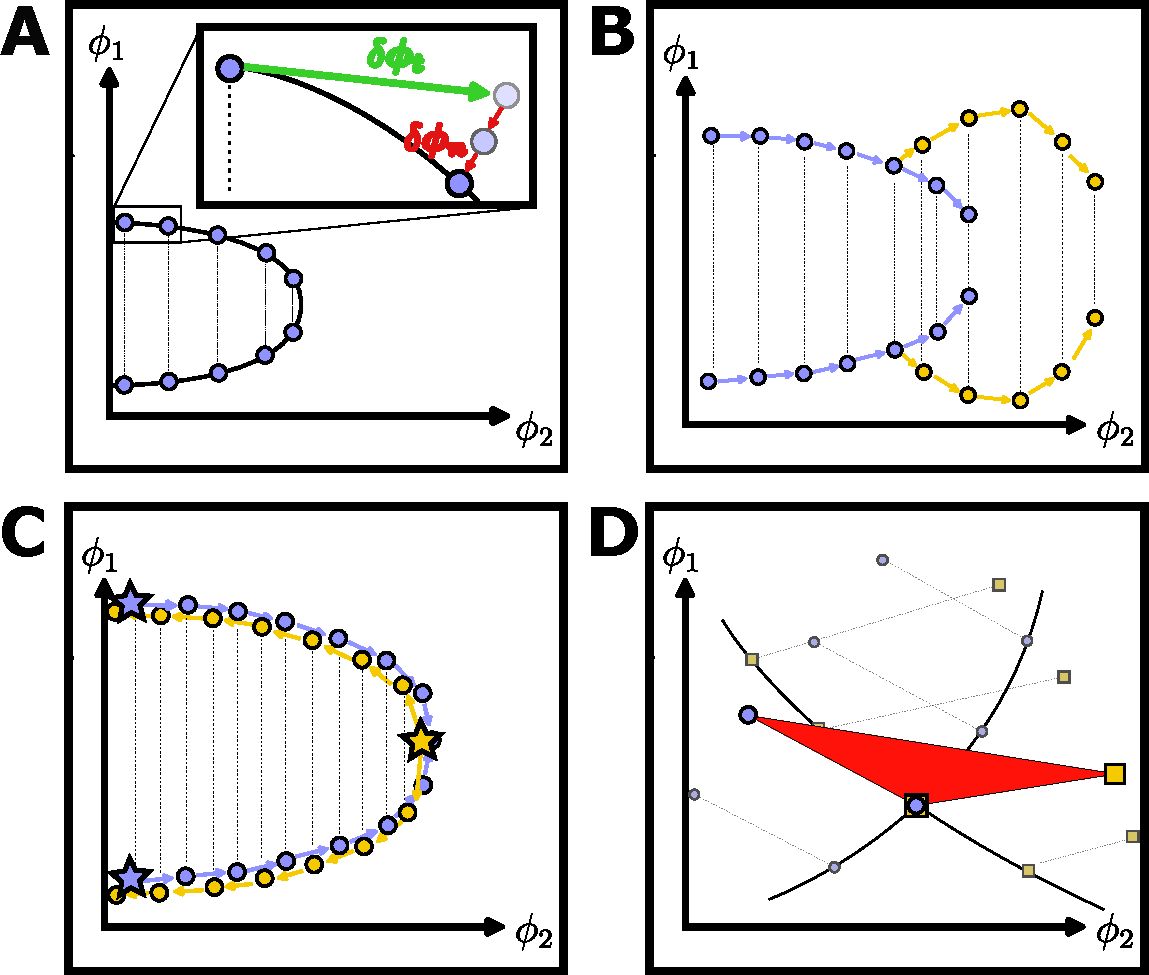
\includegraphics[width=0.98\textwidth]{figures/tracer_schematics.pdf}
    \captionof{figure}{Schematic illustration of the main steps and characteristic events in the algorithm, shown in the \(\phi_1\)-\(\phi_2\) phase space. (A) Successive tangential (green arrow) and projection (red arrow) steps; the projection step may need to be repeated. (B) Branching event: an initial binodal section (blue) splits into a second section (orange) when the Jacobian becomes degenerate. (C) Duplicate binodal sections obtained when tracing is initiated either from the dilute limit (blue points) or from the critical point (orange points). The stars denote the initial points of the tracing processes. (D) The crossing of two binodal sections indicates a three-phase region (orange triangle).}
    \label{fig:tracer_schematics}
\end{minipage}\\

\subsubsection{Identification of three-phase regions}
We now identify three-phase regions by searching for intersections between distinct sections of the binodal.
Such an intersection indicates the existence of a composition that serves as a common endpoint of two tie-lines.
If one composition coexists with two others in this way, then all three compositions satisfy the same coexistence conditions and therefore represent three coexisting phases.

Geometrically, these three phases define a common tangent plane that touches the free-energy surface at three distinct points and forms the convex envelope of the free-energy surface in this region, shown by the orange triangle in Fig.~\ref{fig:three_phase_intuition}.
\noindent
\begin{minipage}{0.1\textwidth}
\end{minipage}\hfill

\begin{minipage}{0.8\textwidth}
    \centering
    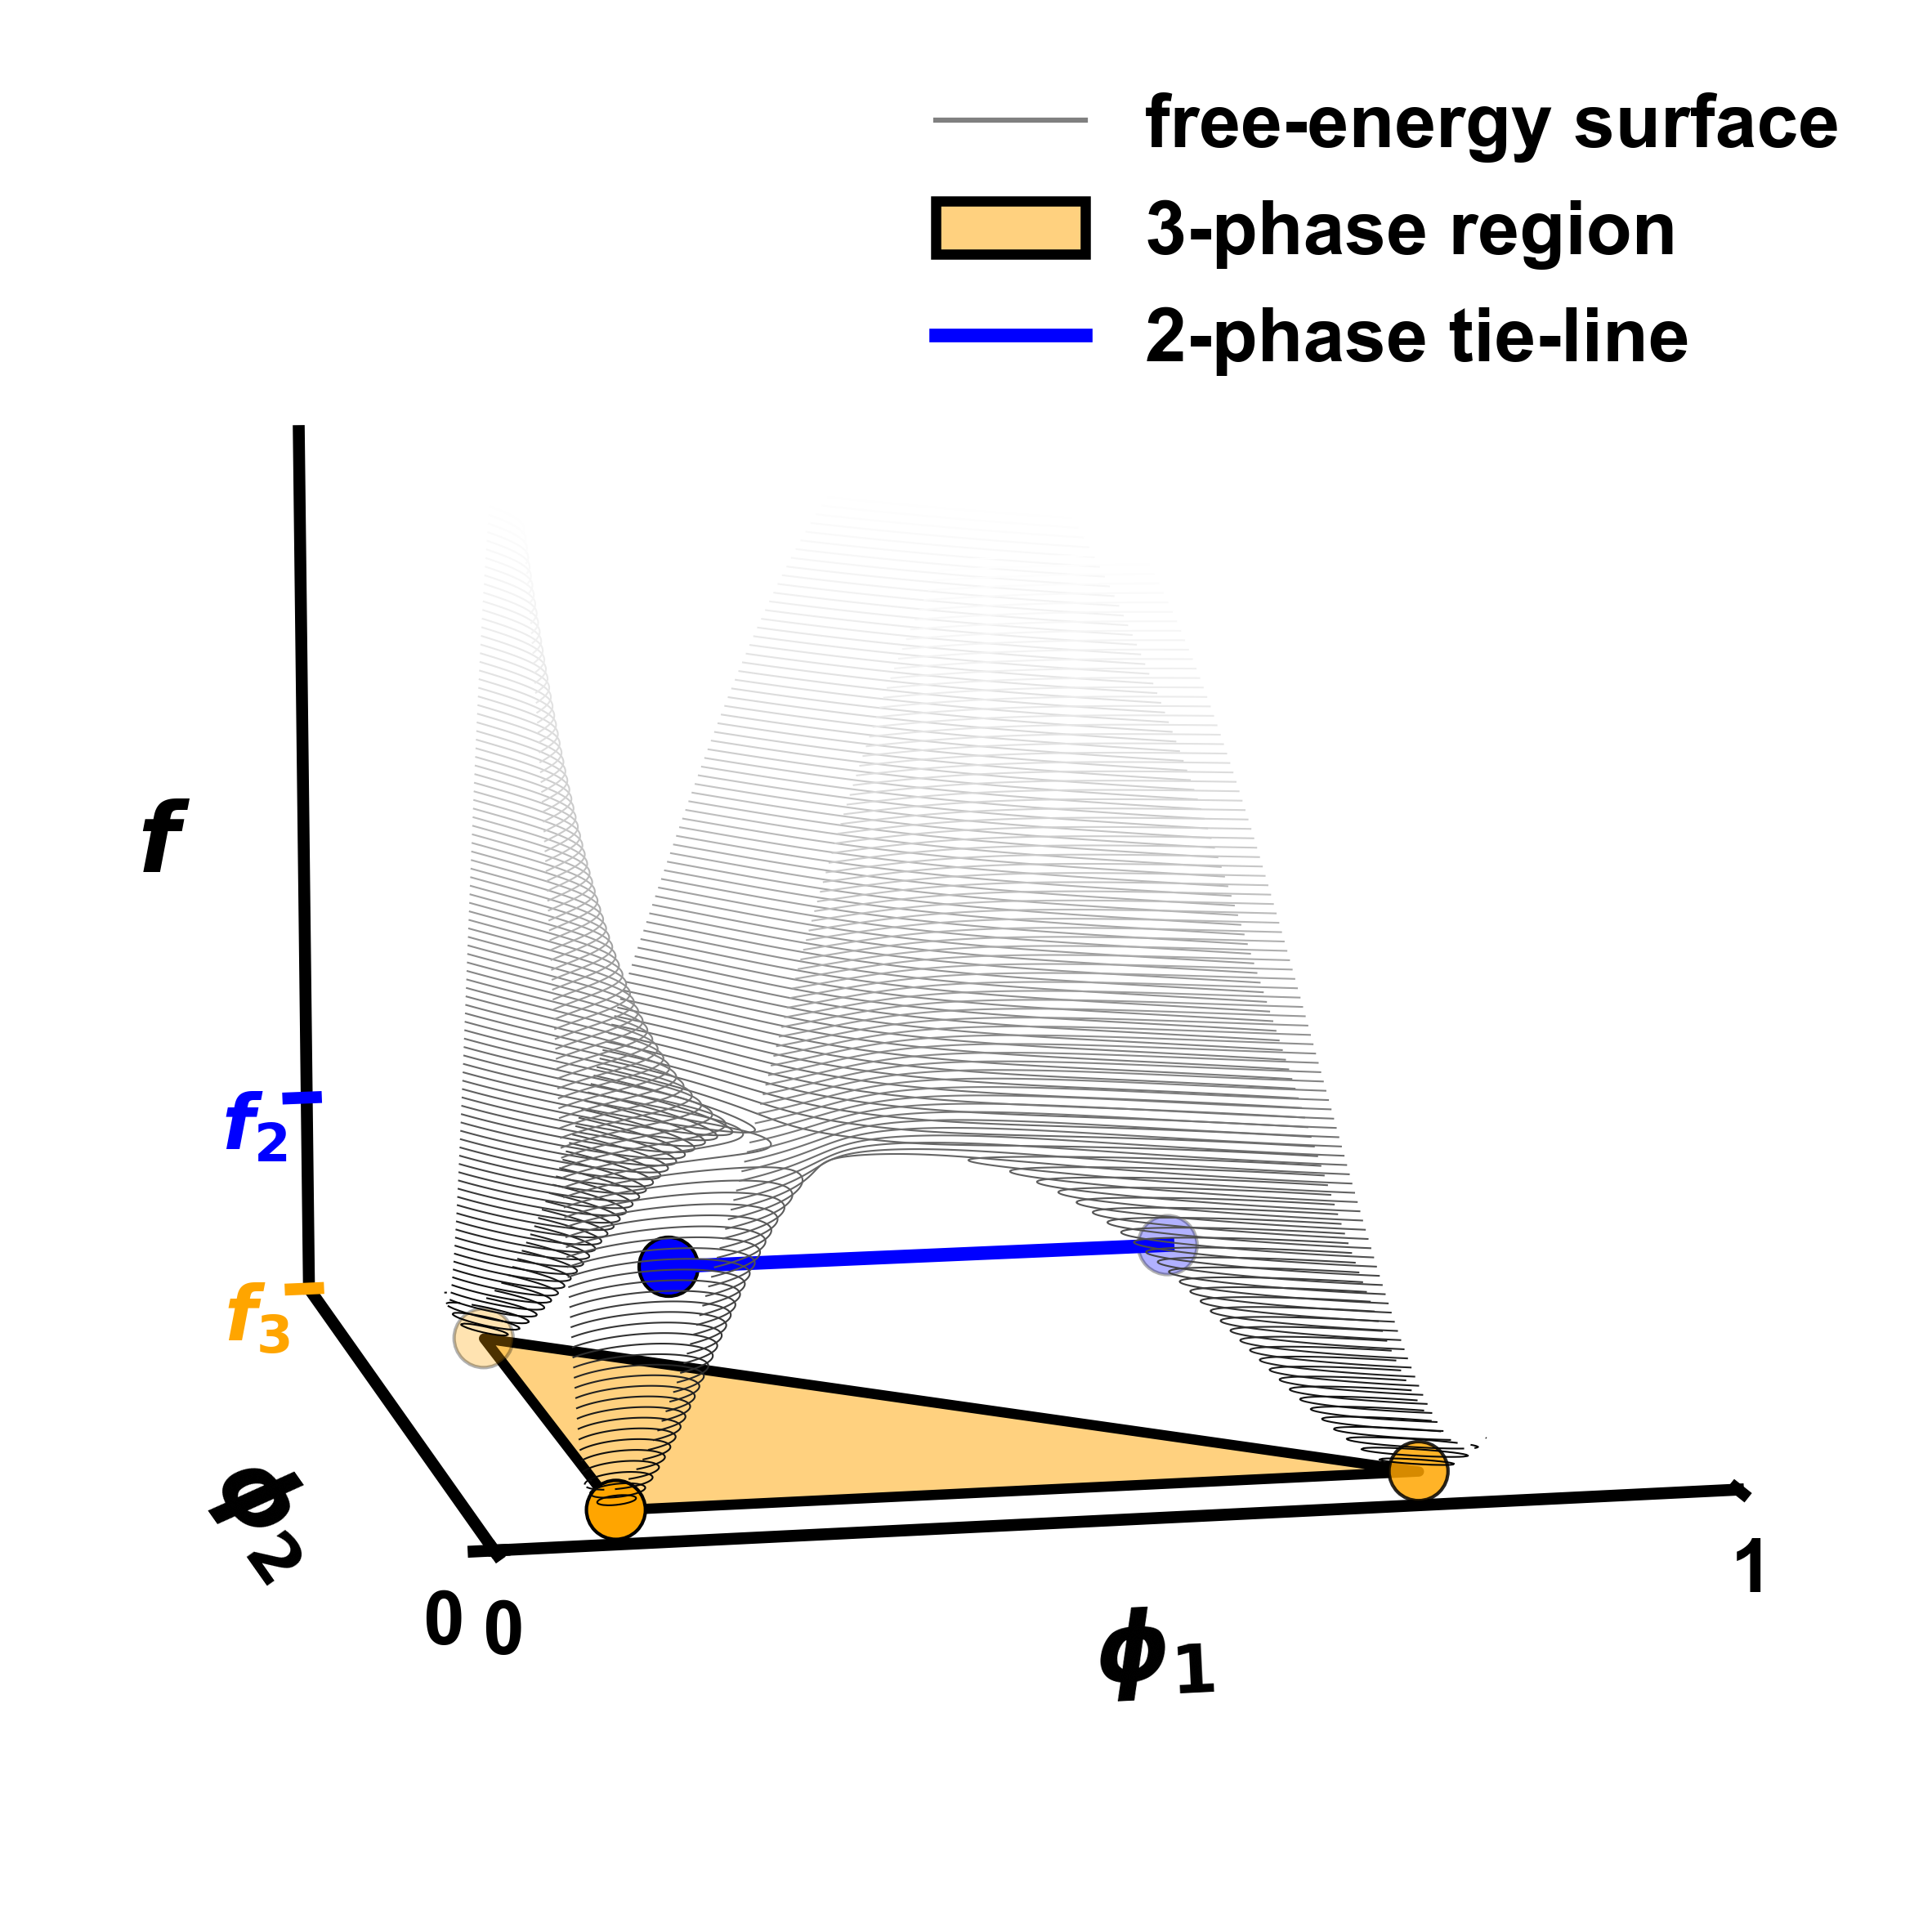
\includegraphics[width=\textwidth]{figures/three_phase_intuition.png}
    \captionof{figure}{Free-energy surface (gray contours) in composition space. The three-phase region (orange triangle) provides a better convexification of the free-energy surface than the two-phase tie-line (blue line). Therefore, a three-phase decomposition always yields a lower free-energy \(f_3\) than a two-phase decomposition \(f_2\).\\}
    \label{fig:three_phase_intuition}
\end{minipage}\hfill
\\The key thermodynamic point is that, within this region, a three-phase decomposition yields a lower free-energy than any competing two-phase decomposition.
To show this, consider a composition \(\boldsymbol{\phi}\) decomposed by the lever rule into either \(N_p=2\) or \(N_p=3\) coexisting phases,
\[
\boldsymbol{\phi} = \sum_{i=1}^{N_p} \lambda_{i,N_p} \boldsymbol{\phi}^{(i,N_p)},
\qquad
\sum_{i=1}^{N_p} \lambda_{i,N_p} = 1,
\qquad
\lambda_{i,N_p} > 0.
\]
Here, \(\boldsymbol{\phi}^{(i,N_p)}\) denotes the composition of phase \(i\) in an \(N_p\)-phase decomposition, and \(\lambda_{i,N_p}\) the corresponding lever-rule coefficients, i.e. the phase fractions.

For a three-phase decomposition, any composition inside the three-phase region satisfies
\begin{equation}
f(\boldsymbol\phi) \geq \sum_{i=1}^3 \lambda_{i,3} f(\boldsymbol{\phi}^{(i,3)}) \eqcolon f_3,
\label{eq:three_phase_free_energy}
\end{equation}
where the \(\lambda_{i,3}\) are the corresponding lever-rule coefficients.
Thus, the free-energy of the original composition is bounded from below by that of the three-phase decomposition.

Now consider an arbitrary two-phase decomposition of the same composition. Its free-energy is
\[
f_2 \coloneq \sum_{i=1}^2 \lambda_{i,2} f(\boldsymbol{\phi}^{(i,2)})
\geq
\sum_{i=1}^2 \lambda_{i,2}\sum_{j=1}^3 \bar\lambda_{ij,3} f(\boldsymbol{\phi}^{(j,3)})
=
\sum_{j=1}^3 \lambda_{j,3} f(\boldsymbol{\phi}^{(j,3)})
=
f_3.
\]
In the second step, each two-phase composition \(\boldsymbol{\phi}^{(i,2)}\) was itself decomposed into the three coexisting phases using Eq.~\eqref{eq:three_phase_free_energy}. In the third step, we introduced the relation
\[
\lambda_{j,3} = \sum_{i=1}^2 \lambda_{i,2} \bar\lambda_{ij,3}.
\]


Consequently, whenever a three-phase construction exists, it is energetically favored over any two-phase separation.
This is illustrated in Fig.~\ref{fig:three_phase_intuition}, where the orange triangle lies below the blue tie-line in free-energy.

Finally, we do not need to consider the possibility of four or more coexisting phases, because within the present ternary setting Gibbs phase rule \cite{GibbsPhaseRule} permits at most three coexisting phases. 

\subsection{Implementation}

Within Flory-Huggins theory, the phase diagram of a ternary system is fully determined by the interaction parameters \(\chi_{ij}\) (we restrict attention to the case of equal molecular sizes).
Accordingly, the only physical input required by our algorithm is the set of interaction parameters from which the phase diagram is constructed.
All other parameters are numerical and control aspects of the implementation such as step sizes, tolerances and convergence behavior.
When chosen appropriately, they do not change the underlying phase behavior, but they do affect how robustly and completely the phase diagram is reconstructed. 
A table of all numerical hyperparameters of this algorithm is provided in the Appendix (see Table~\ref{tab:numerical_parameters}).


\subsubsection{Computing the phase diagram}

Once the interaction parameters are specified, the spinodal curve and the critical points are computed first.
For the Flory-Huggins free-energy density, both can be obtained analytically (see Subsection~\ref{ss:thermodynamics}).
Together with the dilute-limit constructions described above, the critical points determine the initial continuation tasks from which the binodal sections are traced.
A continuation task is the pair \((\boldsymbol{\phi}, \delta\boldsymbol{\phi}_t)\), consisting of a four dimensional phase-space point \(\boldsymbol{\phi}\) and a continuation direction \(\delta\boldsymbol{\phi}_t\) specifying which local section to follow.

All initial continuation tasks are collected in a task list.
The algorithm then repeatedly selects a task from this list and traces the associated section.
During this tracing process, the singular values of the Jacobian are monitored in order to detect branching events.
To avoid stepping over a branching event, the tangential step size is adjusted dynamically according to the value of the second smallest singular value.
Whenever the second smallest singular value falls below a prescribed threshold, this signals that an additional section may emanate from the current point.
In that case, a new continuation task is created from the current phase-space point together with the continuation direction not being followed by the current section, and this task is added to the task list.

In this way, the algorithm gradually discovers and explores all connected sections of the binodal.
After the sections initialized from the dilute limits and critical points have been processed, the remaining sections are generated automatically through the detected branching events.
The procedure continues until the task list is empty. To avoid tracing the same section multiple times, previously explored continuation tasks are cached and duplicate tasks are skipped when encountered.

Executing a continuation task means repeatedly taking a tangential step along the binodal and then projecting the predicted point back onto the coexistence manifold using the pseudoinverse of the Jacobian.
This continuation is repeated until one of the following termination criteria is met:

\begin{terminationbox}
\begin{itemize}
    \item One of the volume fractions leaves the physically admissible range between 0 and 1.
    \item A critical point is reached, which is detected when the distance between the two coexisting phases falls below a prescribed threshold.
    \item In rare cases, the binodal can loop back onto itself, which may lead to an infinite continuation cycle (see Figure~\ref{fig:self_loop} in the Appendix). To avoid this, the distance between the current point and the initial point is monitored and the procedure is terminated once this distance drops below a prescribed threshold.
\end{itemize}
\end{terminationbox}
The full workflow of the algorithm is summarized below.


\begin{tcolorbox}[colback=blue!6,colframe=blue!45!black,arc=2.5mm,title={Pseudocode: Computing the phase diagram},fonttitle=\bfseries]
\begin{algorithmic}[1]
\State $\mathrm{task\_list} \gets \mathrm{ComputeInitialTasks}(\chi)$
\State $\mathrm{history\_list} \gets [\ ]$
\While{$\mathrm{task\_list}$ is not empty}
    \State $\mathrm{task} \gets \mathrm{task\_list}.\mathrm{pop\_first}()$
    \If{$\mathrm{InHistory}(\mathrm{task}, \mathrm{history\_list})$}
        \State \textbf{continue}
    \EndIf
    \State $\mathrm{history\_list}.\mathrm{append}(\mathrm{task})$
    \State $(\mathrm{section}, \mathrm{branch\_tasks}) \gets \mathrm{ComputeBinodalSection}(\mathrm{task})$
    \State $\mathrm{StoreSection}(\mathrm{section})$
    \ForAll{$\mathrm{task_new} \in \mathrm{branch\_tasks}$}
        \State $\mathrm{task\_list}.\mathrm{append}(\mathrm{task_new})$
    \EndFor
\EndWhile
\State $\mathrm{PostProcessing}()$

\Statex
\Function{ComputeBinodalSection}{$\mathrm{task}$}
    \State $(p, d) \gets \mathrm{task}$
    \State $\sigma \gets \mathrm{SingularValuesOfJacobian}(p)$
    \State $\mathrm{section} \gets [p]$, $\mathrm{sv\_list} \gets [\ ]$
    \While{termination criteria are not met}
        \State $d \gets \mathrm{ComputeTangentialDirection}(p, d, \sigma)$
        \State $p \gets p + d$
        \While{$\|\boldsymbol{E}(p)\|$ is above projection threshold}
            \State $p \gets p + \mathrm{ComputeProjectionCorrection}(p)$
        \EndWhile
        \State $\sigma \gets \mathrm{SingularValuesOfJacobian}(p)$
        \State $\mathrm{sv\_list}.\mathrm{append}(\sigma)$
        \State $\mathrm{section}.\mathrm{append}(p)$
    \EndWhile
    \State $\mathrm{branch\_tasks} \gets \mathrm{DetectBranchPoints}(\mathrm{section}, \mathrm{sv\_list})$
    \State \Return $(\mathrm{section}, \mathrm{branch\_tasks})$
\EndFunction
\end{algorithmic}
\end{tcolorbox}

\subsubsection{Post processing}
After all binodal sections have been computed, one needs to remove duplicates, which can occur, for example, if tracing is started both at the boundary of the phase diagram and at the critical point of the same binodal section (see Fig.~\ref{fig:tracer_schematics}C).
Once all duplicates are removed, one can look for intersecting points of two sections of the binodal, since such intersections signal the existence of a three-phase region (see Fig.~\ref{fig:tracer_schematics}D).




\subsection{Results and validation}
The resulting phase diagram consists of the spinodal and binodal sections together with the dividing lines between the one-phase, two-phase, and three-phase regions in composition space.
An example can be seen in Fig.~\ref{fig:algo_example_diagram}B.\\
Figure~\ref{fig:algo_example_diagram}A serves as a guide to reading ternary phase diagrams.

\noindent
\begin{minipage}{0.95\textwidth}
    \centering
    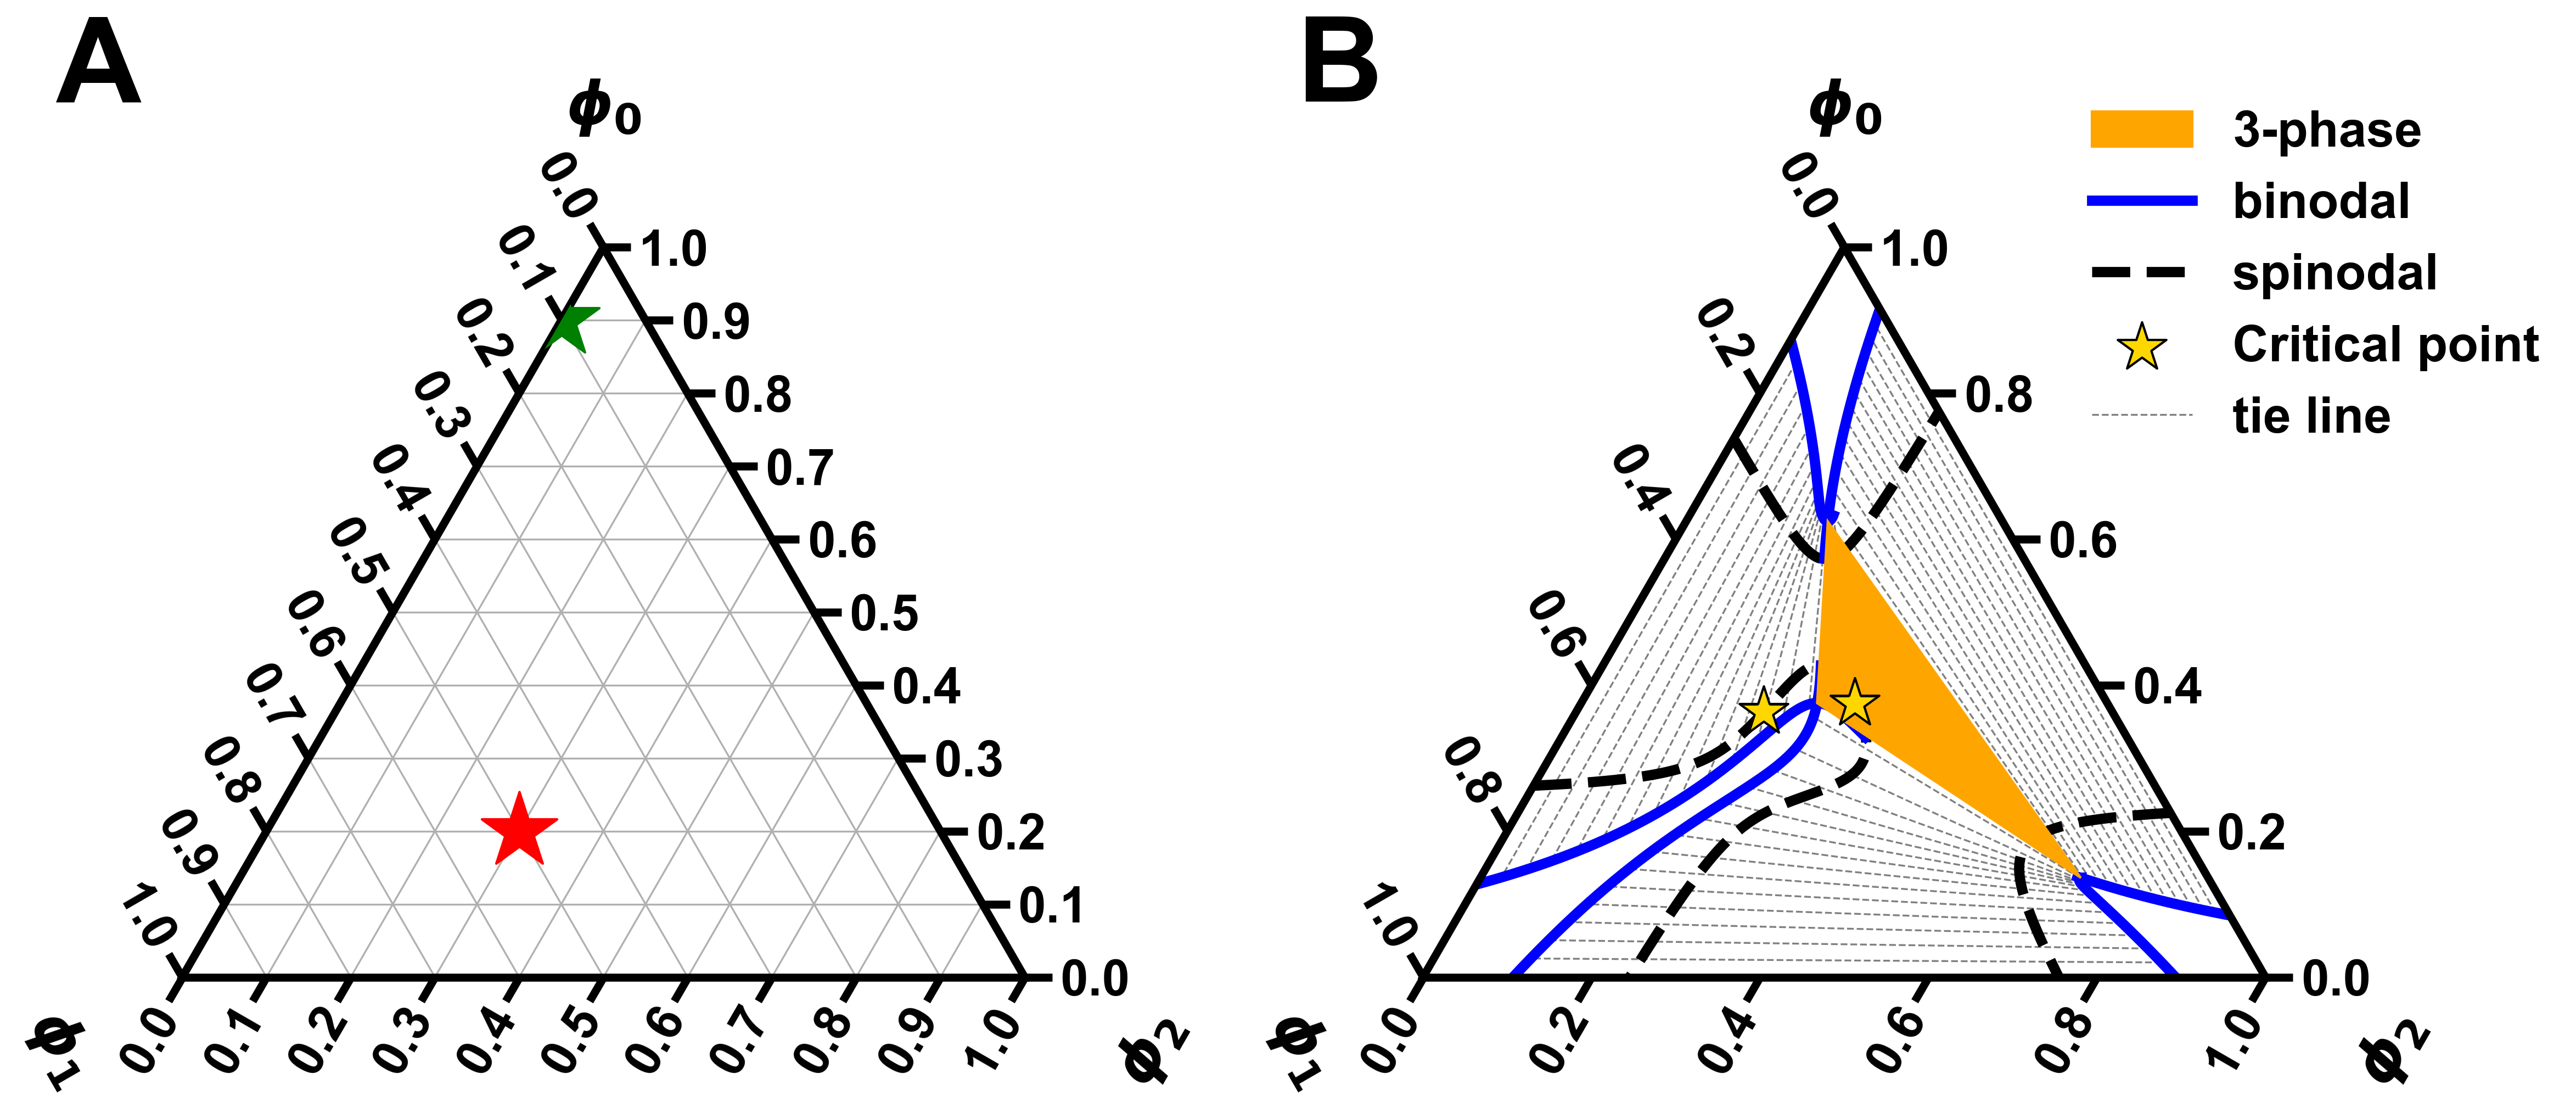
\includegraphics[width=\textwidth]{figures/algo_example_diagram.png}
    \captionof{figure}{(A) Ternary diagram, with axes \(\phi_0\) on the right diagonal, \(\phi_1\) on the left diagonal and \(\phi_2\) on the horizontal axis. The red star is at \((\phi_0\,\phi_1\,\phi_2)^T=(0.2\,0.5\,0.3)^T\) and the green star is at \((\phi_0\,\phi_1\,\phi_2)^T=(0.9\,0.1\,0.0)^T\). Note that the sum of the three volume fractions is always 1.\\
     (B) Phase diagram for \((\chi_{01},\chi_{02},\chi_{12})=(2.6,2.9,2.7)\), showing the spinodal (thick dashed line), binodal (blue line), three-phase region (orange areas), critical point (gold stars) and tie-lines (gray dashed lines).}
    \label{fig:algo_example_diagram}
\end{minipage}


\subsubsection{Validation of the algorithm}
There are several aspects of the algorithm that can be verified. The most obvious check is whether the two-phase coexistence compositions obtained from the continuation scheme satisfy the coexistence conditions, as this defines the binodal.
Owing to the projection step, this is guaranteed (up to numerical tolerance).
Similarly three-phase compositions will satisfy the coexistence conditions as well, since they are the union of two pairs of two-phase states.

A more demanding question is whether the algorithm identifies all phase-separated states in the phase diagram.
In principle, it could miss part of the diagram if, for example, a branching event were not detected.
To test for this possibility, we compare our results against an independent method.
Before developing the present algorithm, we used the \texttt{flory} package \cite{Yicheng2025flory} in the chapter \ref{s:surface_tension} to compute coexistence compositions, and we now use it here for validation.

To this end, we constructed a three-dimensional grid over the interaction parameters \(\chi_{01}, \chi_{02}, \chi_{12} \in [-5, 5]\) and generated $1000$ phase diagrams for the corresponding interaction matrices.
We then sampled random points in composition space and compared the coexistence compositions predicted by our algorithm with those obtained from \texttt{flory}.
The numbers of sampled points in the one-, two- and three-phase regions were chosen in proportion to the respective areas of these regions in composition space. 

In total, we sampled $20000$ two-phase points. For the overwhelming majority of these, \texttt{flory} likewise identified a two-phase coexistence composition.
In those cases, the coexistence compositions were nearly identical.
The only notable deviations occurred near critical points, where \texttt{flory} sometimes identified a larger number of phases, which were nearly identical.
Nonetheless the free-energy differences were below $10^{-6}$. In the parameter regime considered here, all contributions to the Flory-Huggins free-energy density are of order unity, so a difference of $10^{-6}$ is negligible on this scale.

\noindent
\begin{minipage}{0.45\textwidth}
For the three-phase region, we sampled $1000$ points and again found negligible differences, with free-energy differences of order $10^{-6}$.
The only noticeable discrepancy between the two methods occurred near the boundary of a three-phase region.
There, the \texttt{flory} package would occasionally find a two-phase coexistence composition yielding a slightly higher free-energy than the three-phase coexistence composition found by our algorithm (see Fig.~\ref{fig:flory_fails}).


We also sampled $2500$ points in the one-phase region, where no phase separation is expected. In nearly all cases, the \texttt{flory} package likewise found no coexistence compositions, the exception being near the critical point, where again \texttt{flory} would occasionally return multiple phases.
\end{minipage}
\hfill
\begin{minipage}{0.5\textwidth}
    \centering
    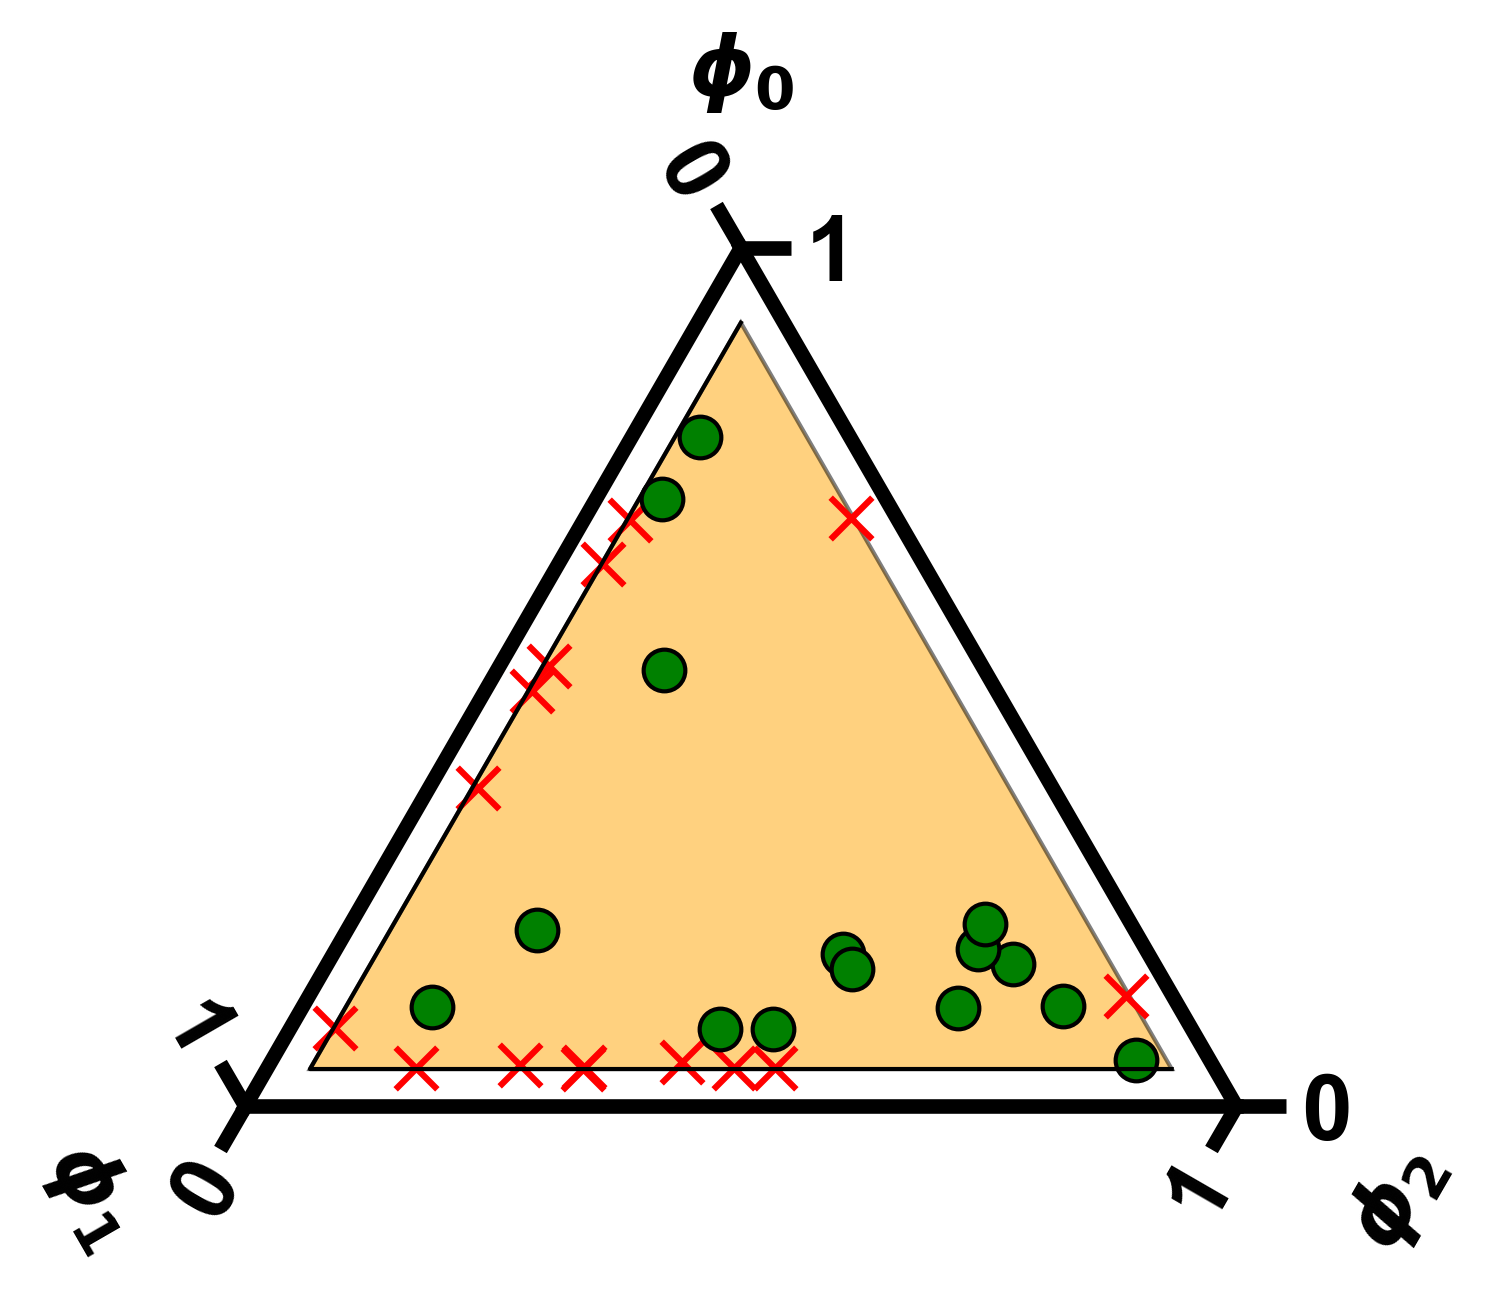
\includegraphics[width=\textwidth]{figures/flory_fails.png}
    \captionof{figure}{Ternary plot of an example system with a three-phase region (orange triangle).
    The green points indicate mean compositions for which both \texttt{flory} and our algorithm predict three-phase coexistence.
    The red crosses indicate mean compositions for which \texttt{flory} predicts two-phase coexistence, whereas our algorithm predicts three-phase coexistence.}
    \label{fig:flory_fails}
\end{minipage}\\

Of course, this is not a proof that the algorithm will work for all possible interaction parameters, but it does provide strong empirical evidence that the algorithm is robust and suitable for exploring representative ternary phase behavior.

\subsubsection{Case study: symmetric ternary system}\label{sss:case_study_symmetric_ternary}
The symmetric ternary case is defined by equal interactions of one species with the other two, \(\chi_{01}=\chi_{02}\), while the interaction between the remaining two species is given by \(\chi_{12}\).
For the purpose of this example, we assume species 0 to interact equally with species 1 and 2. Of course, the same construction applies to the other species after relabeling the species and the corresponding interaction parameters.

An advantage of this case is that the binodals can be computed analytically using a simple ansatz.
We assume that one species has the same composition in both phases, while the remaining two species exchange their volume fractions between phases.
We can write this ansatz as
\[
\begin{aligned}
\phi_0^{(1)}& = \phi_0^{(2)},\\
\phi_1^{(1)}&= \phi_2^{(2)}\eqcolon \phi^{(1)},\\
\phi_1^{(2)}&= \phi_2^{(1)}\eqcolon \phi^{(2)}
\end{aligned}
\]

\noindent
\begin{minipage}{0.45\textwidth}
For this case the coexistence condition for the exchange chemical potential simplifies to
\begin{equation}
\ln\left(\frac{\phi^{(1)}}{\phi^{(2)}}\right) + \chi_{12} (\phi^{(2)}-\phi^{(1)}) = 0
\label{eq:symmetric_implicit}
\end{equation}\\
Thus, for a given \(\phi^{(1)}\), we can find \(\phi^{(2)}\) by solving the implicit equation Eq.~\ref{eq:symmetric_implicit}.
The comparison between our algorithm and the analytical solution is shown in Fig.~\ref{fig:verify_symmetric}.
In the bottom panel, the difference between the exact coexistence compositions and our algorithmic results is nearly zero, with a maximum absolute error of order \(10^{-8}\), 
The figure is shown for a particular choice of \(\chi_{12}\), but the same level of agreement was obtained for other values of \(\chi_{12}\in[2,3]\).
It is therefore safe to conclude that the algorithm is able to accurately capture the binodal curve for this symmetric ternary system.\\

\end{minipage}
\hfill
\begin{minipage}{0.5\textwidth}
    \centering
    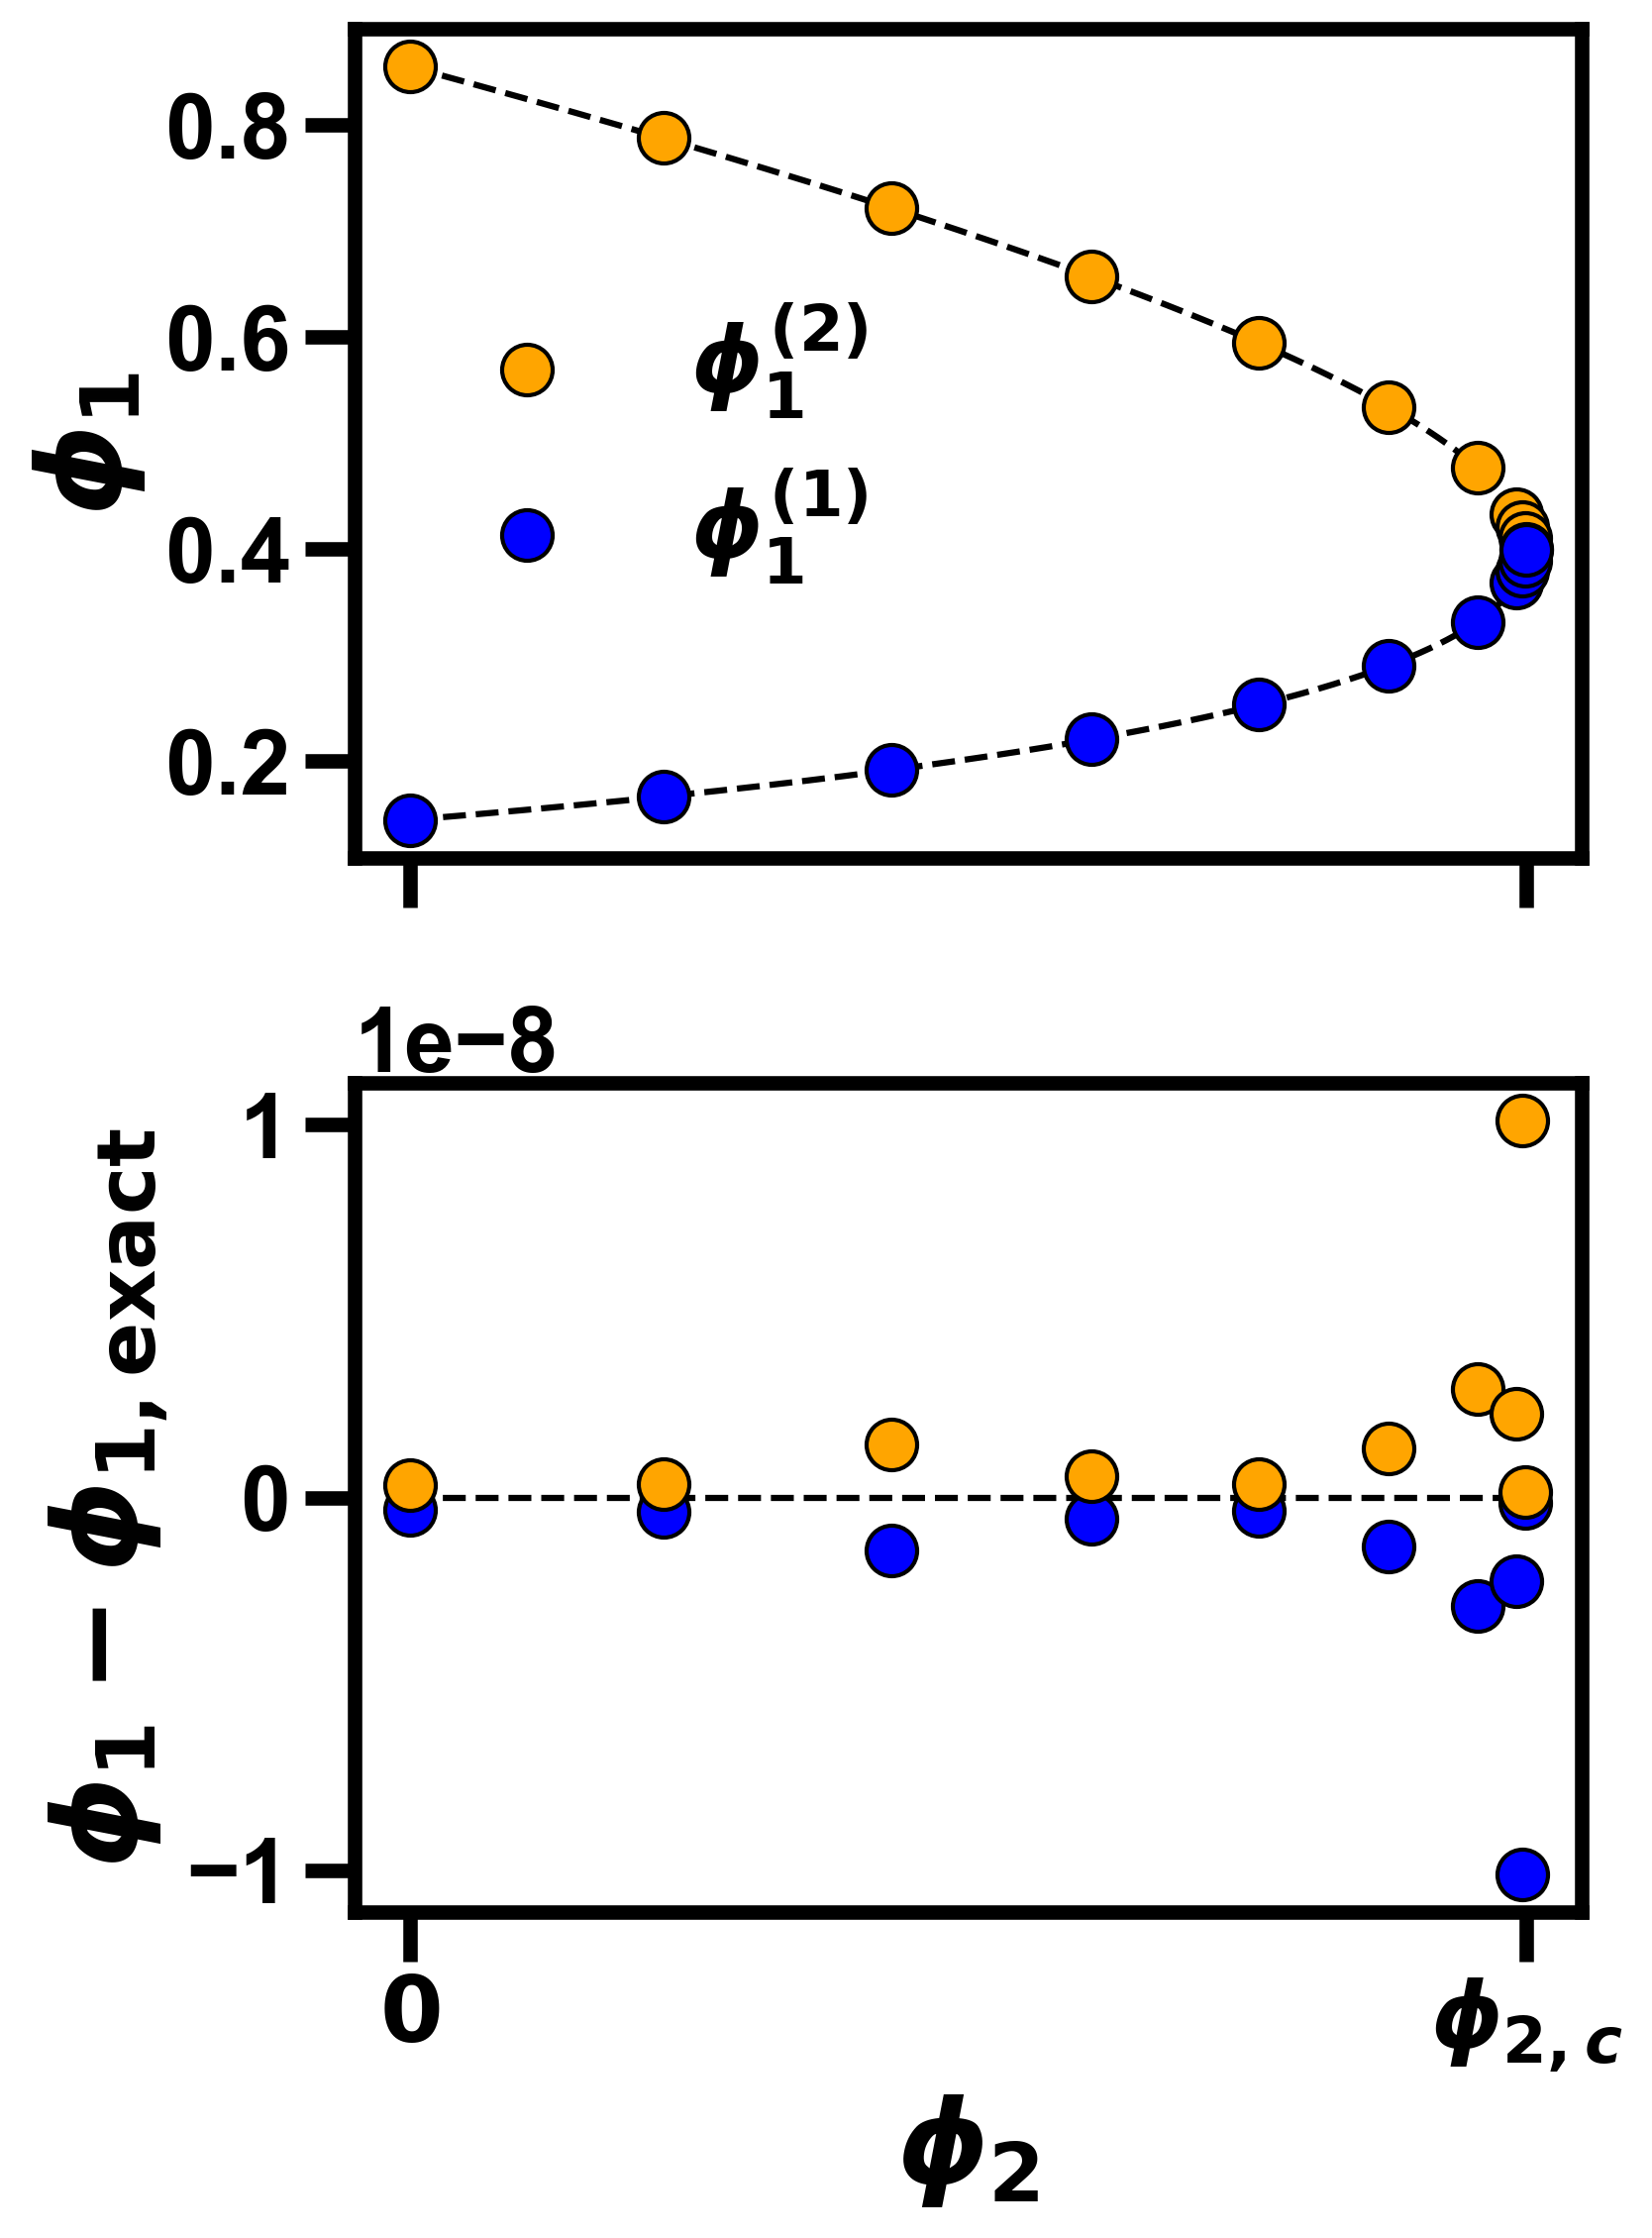
\includegraphics[width=\linewidth]{figures/verify_symmetric.png}
    \captionof{figure}{Top: Binodal curve for the symmetric ternary system with \(\chi_{01}=\chi_{02}=1.5\) and \(\chi_{12}=2.5\). The dashed line shows the analytical solution from Eq.~\ref{eq:symmetric_implicit}, while the blue and orange points show the results obtained with our algorithm. Bottom: The residual between the analytical and numerical results is negligible.\\}

    \label{fig:verify_symmetric}
\end{minipage}\\
Next we turn to the special case in which all interactions are equal, \(\chi_{01}=\chi_{02}=\chi_{12}\eqcolon \chi\).
For this fully symmetric system, previous work \cite{Huang1995PhaseSeparation} provides results that can be used to verify our algorithm, at least qualitatively, since the results are only shown in figures.
In their work, the authors consider several interaction regimes and find a rich variety of phase-diagram topologies for \(\chi \in [2, 3]\) which the present in figure 1 of \cite{Huang1995PhaseSeparation}.
Here we reproduced those figures using our algorithm and find good qualitative agreement, for the different regimes as we will describe now.\\

For \(2<\chi<2.575\) three binodal sections exist originating from the three dilute limits, which enclose the spinodal (see Fig.~\ref{fig:symmetric_chis}A). At \(\chi = 2.575\), one of the binodal sections intersects the spinodal.
Beyond this point, additional binodal sections appear and enclose the spinodal again.
Additionally, the number of critical points increases from $3$ to $9$. In the regime \(2.575< \chi < 2.7\) there are three three-phase regions (Fig.~\ref{fig:symmetric_chis}B).
At \(\chi = 8/3\) the spinodal sections collide and $6$ of the $9$ critical points disappear (Fig.~\ref{fig:symmetric_chis}C).
For \(\chi > 8/3\) there are only three critical points left (Fig.~\ref{fig:symmetric_chis}D).
Finally at \(\chi=2.746\) the three three-phase regions join to a single three-phase region (Fig.~\ref{fig:symmetric_chis}E)
As one increases \(\chi\) further, the single three-phase region grows in size (Fig.~\ref{fig:symmetric_chis}F).
Overall, the sequence of topological changes obtained from our algorithm matches the changes descibed in \cite{Huang1995PhaseSeparation} exactly.\\
\begin{minipage}{0.95\textwidth}
    \centering
    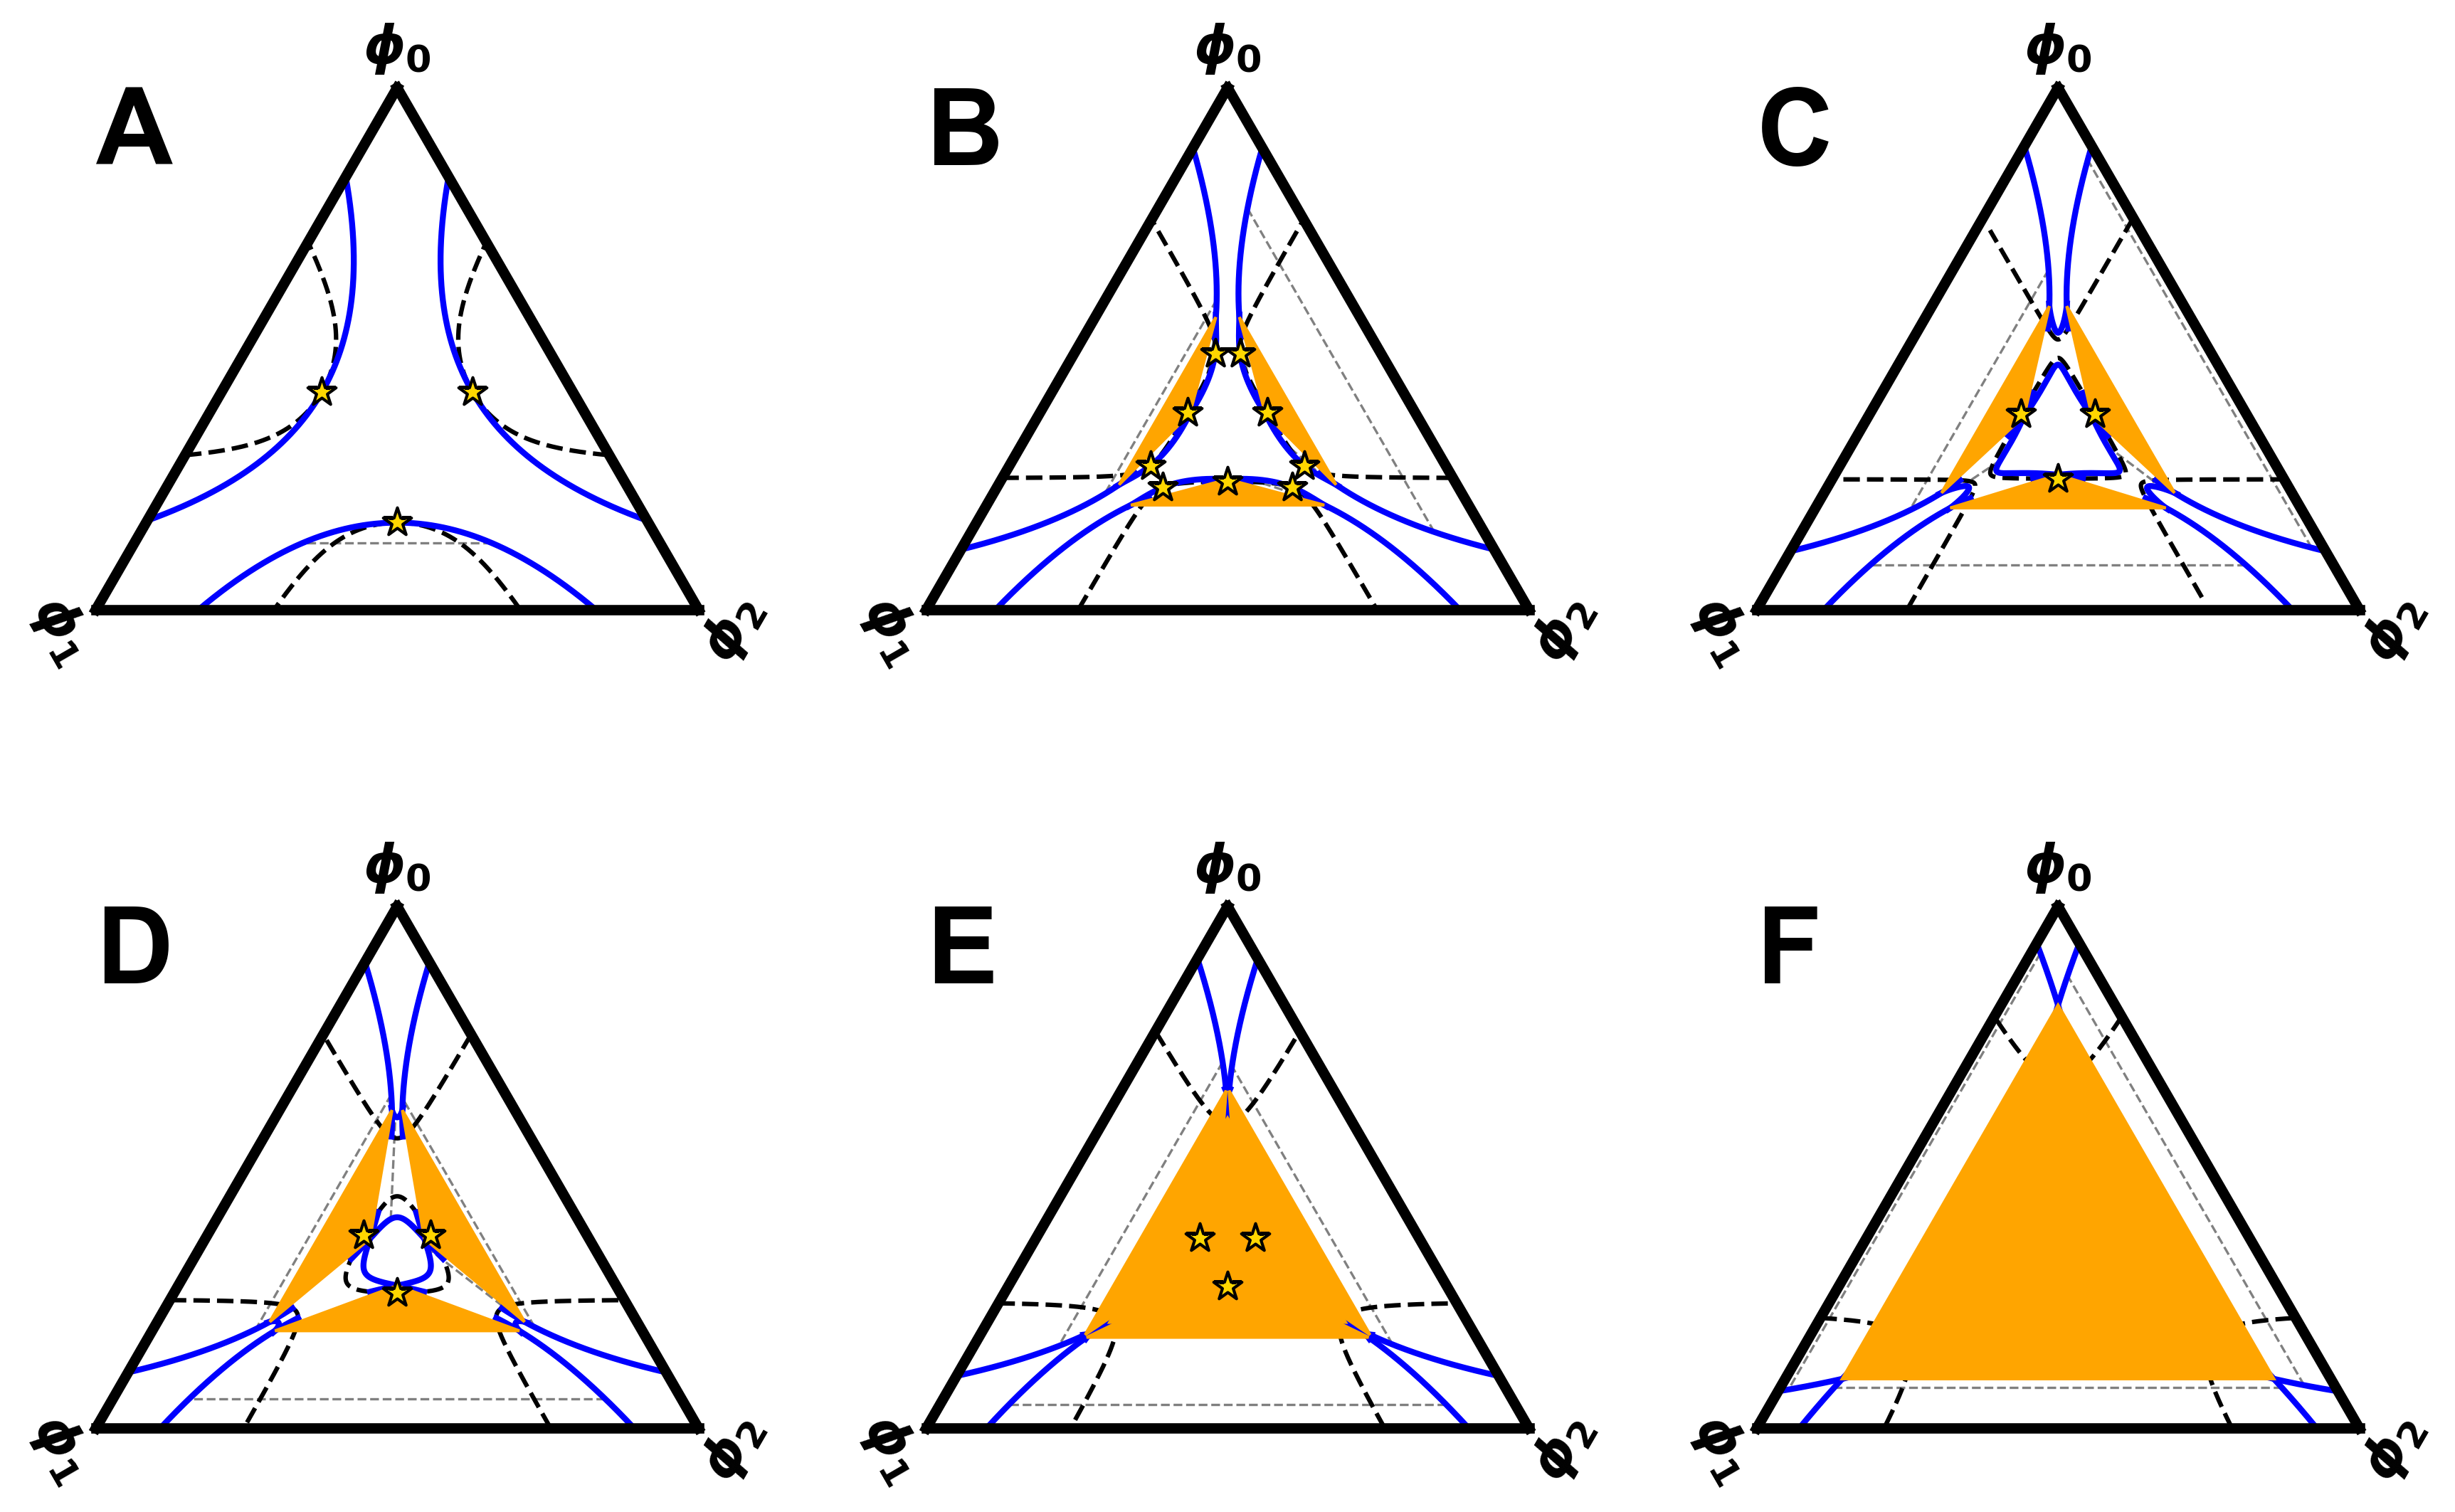
\includegraphics[width=\linewidth]{figures/symmetric_chis.png}
    \captionof{figure}{Phase diagram for different values of \(\chi\).
    The orange triangles are the three-phase regions, the binodal is shown in blue, the spinodal is the thick dashed line, the critical points are the gold stars and the tie-lines are the thin striped lines.
    (A) \(\chi=2.4\), (B) \(\chi=2.65\), (C) \(\chi=8/3\), (D) \(\chi=2.7\), (E) \(\chi=2.746\), (F) \(\chi=3.0\). }
    \label{fig:symmetric_chis}
\end{minipage}\\

\subsubsection{Two interesting classes of phase diagrams}
In the previous example, we focused on a particular class of interaction matrices that yielded a rich variety of phase-diagram topologies as \(\chi\) was varied.
Here, we turn to  the reduced interaction matrix for components \(1\) and \(2\):
\[
\tilde{\chi}=
\begin{pmatrix}
\chi+\delta& \chi-\delta\\
\chi-\delta& \chi+\delta\\
\end{pmatrix}
\]
where we fix $\chi<-4$ and vary $\delta$.
The particular upper limit for \(\chi<\) ensures that the system phase separates at the boundary of the phase diagram.
The reason we are interested in this type of interaction matrix is that two different classes of phase diagrams emerge as the interaction asymmetry parameter \(\delta\) is varied.\\

The first class of phase diagrams is characterized by the absence of critical points, with both the spinodal and the binodal connecting opposite parts of the boundary of the phase diagram (Fig.~\ref{fig:interesting_case}A-C).
For $\delta<0$, the binodal is concave (Fig.~\ref{fig:interesting_case}A).
For $\delta=0$, the diagonal and off diagonal of the reduced interaction matrix are equal, and both the binodal and the spinodal become straight (Fig.~\ref{fig:interesting_case}B).
For $\delta>0$, the binodal becomes convex (Fig.~\ref{fig:interesting_case}C).\\
When $\delta$ exceeds $-4-\chi$, the topology changes and phase separation no longer reaches the boundary. We then obtain a second class of phase diagrams in which both the binodal and the spinodal are fully contained within the physically admissible domain.
In this second class, two critical points appear on opposite ends of the phase diagram (see Fig.~\ref{fig:interesting_case}D-F). For $\delta\gg|\chi|$, the overall shape of the phase diagram changes only weakly (Fig.~\ref{fig:interesting_case}E \& F).
In this limit, the entropic contribution becomes negligible compared to the enthalpic contribution, which is proportional to $\delta$.
Therefore the free-energy density is approximately given by
\[
\begin{aligned}
    f  &= \delta\sum_{ij}\phi_i A_{ij} \phi_j,\quad i,j \in \{1,2\}\\
\boldsymbol A &=
\begin{pmatrix}
1& -1\\
-1& 1\\
\end{pmatrix}
\end{aligned}
\]
Thus, changing $\delta$ only rescales the free-energy density and does not affect the coexistence conditions.

\begin{minipage}{0.95\textwidth}
    \centering
    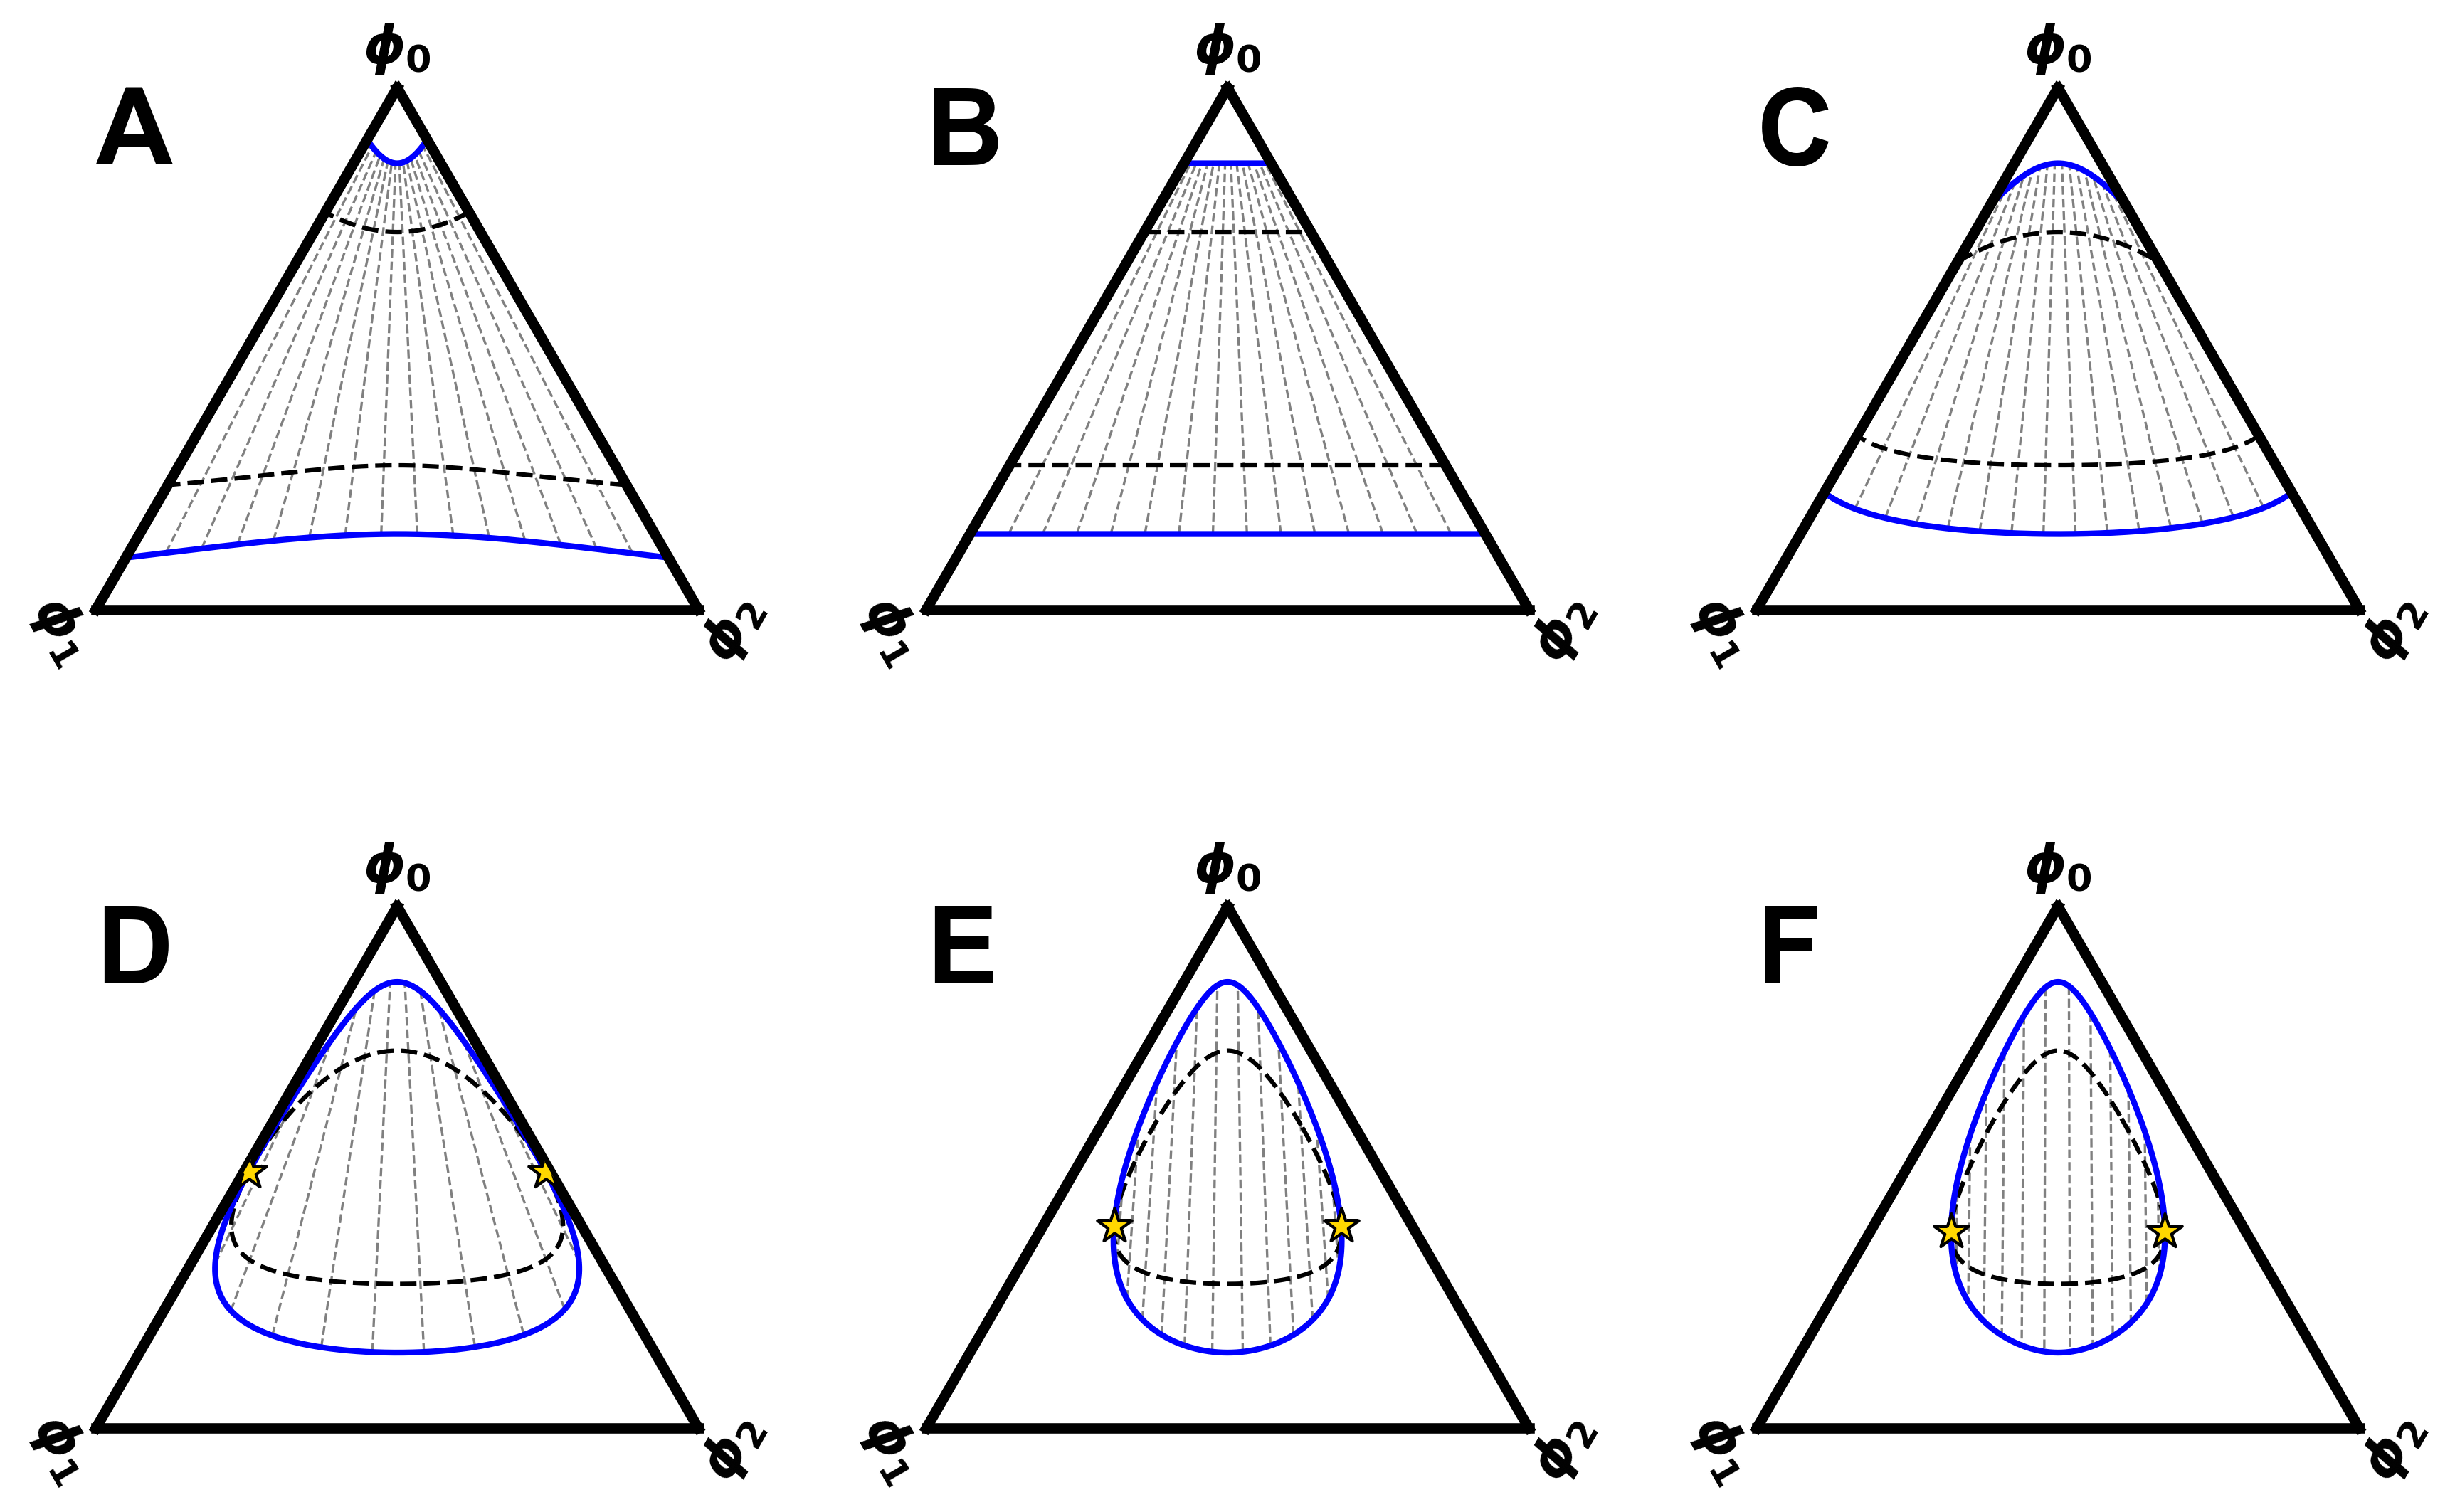
\includegraphics[width=\textwidth]{figures/interesting_case.png}
    \captionof{figure}{Ternary phase diagram for \(\chi=-5\) and varying \(\delta\in[-0.5,60.0]\). Blue line denotes the binodals, the black dashed lines denote spinodal and the gray dashed lines are the tie-lines. (A) \(\delta=-0.5\), (B) \(\delta=0.0\), (C) \(\delta=0.5\), (D) \(\delta=1.1\), (E) \(\delta=10.0\) and (F) \(\delta=60.0\).\\}
    \label{fig:interesting_case}
\end{minipage}\\

A common feature for all phase diagrams in Fig.~\ref{fig:interesting_case} is that the vertical tie-line at the center of the phase diagram is the same for all values of $\delta$.
This tie-line corresponds to the ansatz \(\phi_1 = \phi_2\eqcolon \phi\), which we can insert into the free-energy density to obtain
\[
f= 2\phi \ln(\phi) + (1-2\phi) \ln(1-2\phi) + 2\chi \phi^2.
\]
Thus, the coexistence conditions along this tie-line are independent of $\delta$ and depend only on $\chi$. For \(\chi=-5\), this gives the coexistence compositions \(\phi_{1/2}^{(1)} \approx 0.072\) and \(\phi_{1/2}^{(2)} \approx 0.428\).


\clearpage
\section{Discussion and Outlook}
This thesis addressed two complementary aspects of phase separation in ternary Flory-Huggins mixtures: the structure and energetics of interfaces, and the efficient construction of phase diagrams.
Taken together, these results highlight features unique to ternary systems, both in the global organization of phase space and in the local interfacial physics, and provide a coherent framework for studying three-component liquid-liquid phase separation.\\

In Chapter~\ref{s:surface_tension}, we set out to characterize the interfacial properties of mixtures and found, through a combination of numerical calculations and analytical derivations, that preferential interfacial adsorption is a central feature of ternary interfaces.

We began by computing the surface tension numerically and established the power law \(\gamma \sim |\boldsymbol{\mu}_c-\boldsymbol{\mu}|^{3/2}\), in agreement with the expected critical scaling. A simple analytical approximation, based on linearly interpolating between the two coexisting phases within a common interfacial window, already captures the qualitative behavior of the exact results and, importantly, reproduces the correct scaling near criticality. At the same time, comparison with the numerical profiles makes clear that the main deficiency of this approximation is the neglect of interfacial adsorption, which becomes increasingly important close to the critical point.

The symmetric ternary case made it possible to analyze this effect in greater detail. In that setting, implicit expressions were obtained for the adsorption peak amplitude and the interfacial width, and a hyperbolic-function ansatz provided an accurate representation of the equilibrium profiles. Incorporating the adsorption peak amplitude into the analytical estimate of the surface tension yielded much better agreement with the numerical data, especially in the regime where the original approximation exhibited its largest relative error. This strongly suggests that interfacial adsorption is the dominant correction, while the remaining discrepancy is likely due to the simplified shape of the approximate profiles.\\

The second main result of this thesis is a continuation-based algorithm for the rapid construction of ternary phase diagrams. The method combines tangential predictor steps with a projection back onto the coexistence manifold, making it possible to trace the binodal efficiently and with high numerical accuracy.

The idea of a local stepping scheme is not new and has previously been proposed in \cite{Shcherbakova2023}. The present implementation, however, provides a comprehensive framework for the systematic exploration of the full phase diagram. Moreover, to the best of our knowledge, the projection step has not previously been used in this context and is instrumental in achieving both comparatively large step sizes and high numerical accuracy. Within this framework, several interesting geometric features of ternary phase diagrams became apparent, including branching points of the binodal, self-returning binodal sections, and the appearance of three-phase regions.


Validation against the \texttt{flory} package \cite{Yicheng2025flory} and against analytical results for symmetric cases showed very good agreement. The algorithm also reproduced the rich topological changes of the fully symmetric ternary phase diagram studied in previous work \cite{Huang1995PhaseSeparation}, and revealed interesting classes of phase diagrams for a particular family of interaction matrices.


Although the two chapters treat different aspects of ternary phase separation, together they follow the natural order in which ternary systems are usually analyzed. The phase-diagram algorithm enables the rapid exploration of the phase behavior of a wide range of ternary systems. It can therefore be used to identify promising candidates for the subsequent study of interfacial phenomena.\\

Several natural directions for future work follow from these results. For the interfacial system, we begin with a number of smaller problems that would serve more as extensions of the present thesis than as independent projects. First, it would be interesting to derive the critical exponent of \(3/2\) directly from the exact definition of the surface tension given in Eq.~\ref{eq:surfacetension_flory}, in order to corroborate the results of the simplified approximation. Second, it would be interesting to validate the ans\"atze in Section~\ref{sss:profile_approximation} for the profiles in the symmetric ternary case. For \(\phi_-\), this would likely involve expanding the Euler-Lagrange equation~\eqref{eq:el_symmetric} around the critical point and showing that the resulting equations are solved by the hyperbolic-function ansatz (following a procedure similar to that used in \cite{Getzinger2026}). For \(\phi_+\), one would neglect the second-derivative term in the Euler-Lagrange equation, as was done for the implicit Eq.~\eqref{eq:delta_phi_plus}, and show that the resulting equation is solved by the hyperbolic-function ansatz with the adsorption peak amplitude given by Eq.~\ref{eq:delta_phi_plus}.

A more elaborate project would be to extend the analytical treatment of Section~\ref{sec:symmetric_case} beyond the symmetric case to the general case. One could begin with a perturbative expansion around symmetry. This may reveal ans\"atze for the profiles of general ternary systems, something that has so far only been achieved in narrowly defined settings \cite{Getzinger2026}.\\

For Chapter~\ref{s:binodal_tracing}, several research directions are possible, given the broad relevance of phase diagrams in soft-matter physics. As a comparatively straightforward extension, the algorithm could be applied to other free-energy densities, for example those that incorporate different molecular sizes or a Ginzburg-Landau free energy. This would require modifying only a single function in the code implementation, since the associated calculus, such as the Jacobian, is computed using automatic differentiation \cite{jax2018github}.

A more challenging endeavor would be to extend the method to systems with more than three components. The current algorithm relies on the coexistence manifold being one-dimensional, with its dimensionality determined by the number of degrees of freedom minus the number of coexistence conditions. Tracing higher-dimensional manifolds would be considerably more difficult. Therefore, the number of degrees of freedom and constraints should be balanced such that the coexistence manifold remains one-dimensional.

A possible strategy would be to introduce additional constraints and trace lower-dimensional slices of the coexistence manifold. For example, suppose one is interested in the two-phase coexistence of a four-component incompressible system. In that case, there are \((N_c-1)\cdot 2 = 6\) degrees of freedom and \(N_c = 4\) coexistence conditions. If one then fixes the mean volume fraction of the solute, this introduces an additional constraint that reduces the coexistence manifold to a one-dimensional curve, which can be traced using the current implementation of the algorithm. Alternatively, one could focus on higher-phase coexistence problems for which the manifold becomes one-dimensional again. For instance, in a four-component system with three-phase coexistence, the manifold again is one-dimensional.

However, having too many degrees of freedom may not necessarily be a disadvantage. A possible future project would be to investigate the binodal of higher-component systems while effectively treating them as ternary systems.
This would be done by labeling three species as input species and the remaining species as hidden species. For a given two-phase coexistence composition, the null space of the Jacobian is higher-dimensional, due to the hidden species. This would make it possible to take a tangential step in an arbitrary direction within the subspace of the input species by expressing the step as a linear combination of the null-space vectors.
In principle, this would make it possible to move the coexistence composition to an arbitrary point within the subspace of the input species, while simultaneously adjusting the composition of the hidden species. Extending this procedure to all two-phase coexistence compositions, i.e. to the entire binodal, may then allow the binodal curve of the input species to be engineered toward a desired shape. This project idea is inspired by the work of \cite{zentner2025informationprocessingdrivenmulticomponent}, who presented a simple neural-network task for multicomponent phase-separating systems.

A different extension of the algorithm would be to include the interaction parameters themselves as degrees of freedom that can be varied during the continuation process. For the ternary case, this would increase the number of degrees of freedom from 4 to 7, so that the null space of the Jacobian becomes four-dimensional. Then, by analyzing the eigenspectrum of the null space of the Jacobian, one could identify the direction in interaction-parameter subspace that induces the largest change in the coexistence compositions. In other words, one could quantify how sensitive a coexistence state is to external perturbations.
This type of extension is inspired by the work of \cite{Qian2024}, which introduced a framework for quantifying the relative energetic contribution, or dominance, of individual components to phase separation.



\clearpage
\bibliographystyle{plain}
\bibliography{references}
\clearpage
\section{Appendix}
\begin{itemize}
    \item Plot of self-returning binodal section
\end{itemize}
\begin{minipage}{\textwidth}
    \centering
    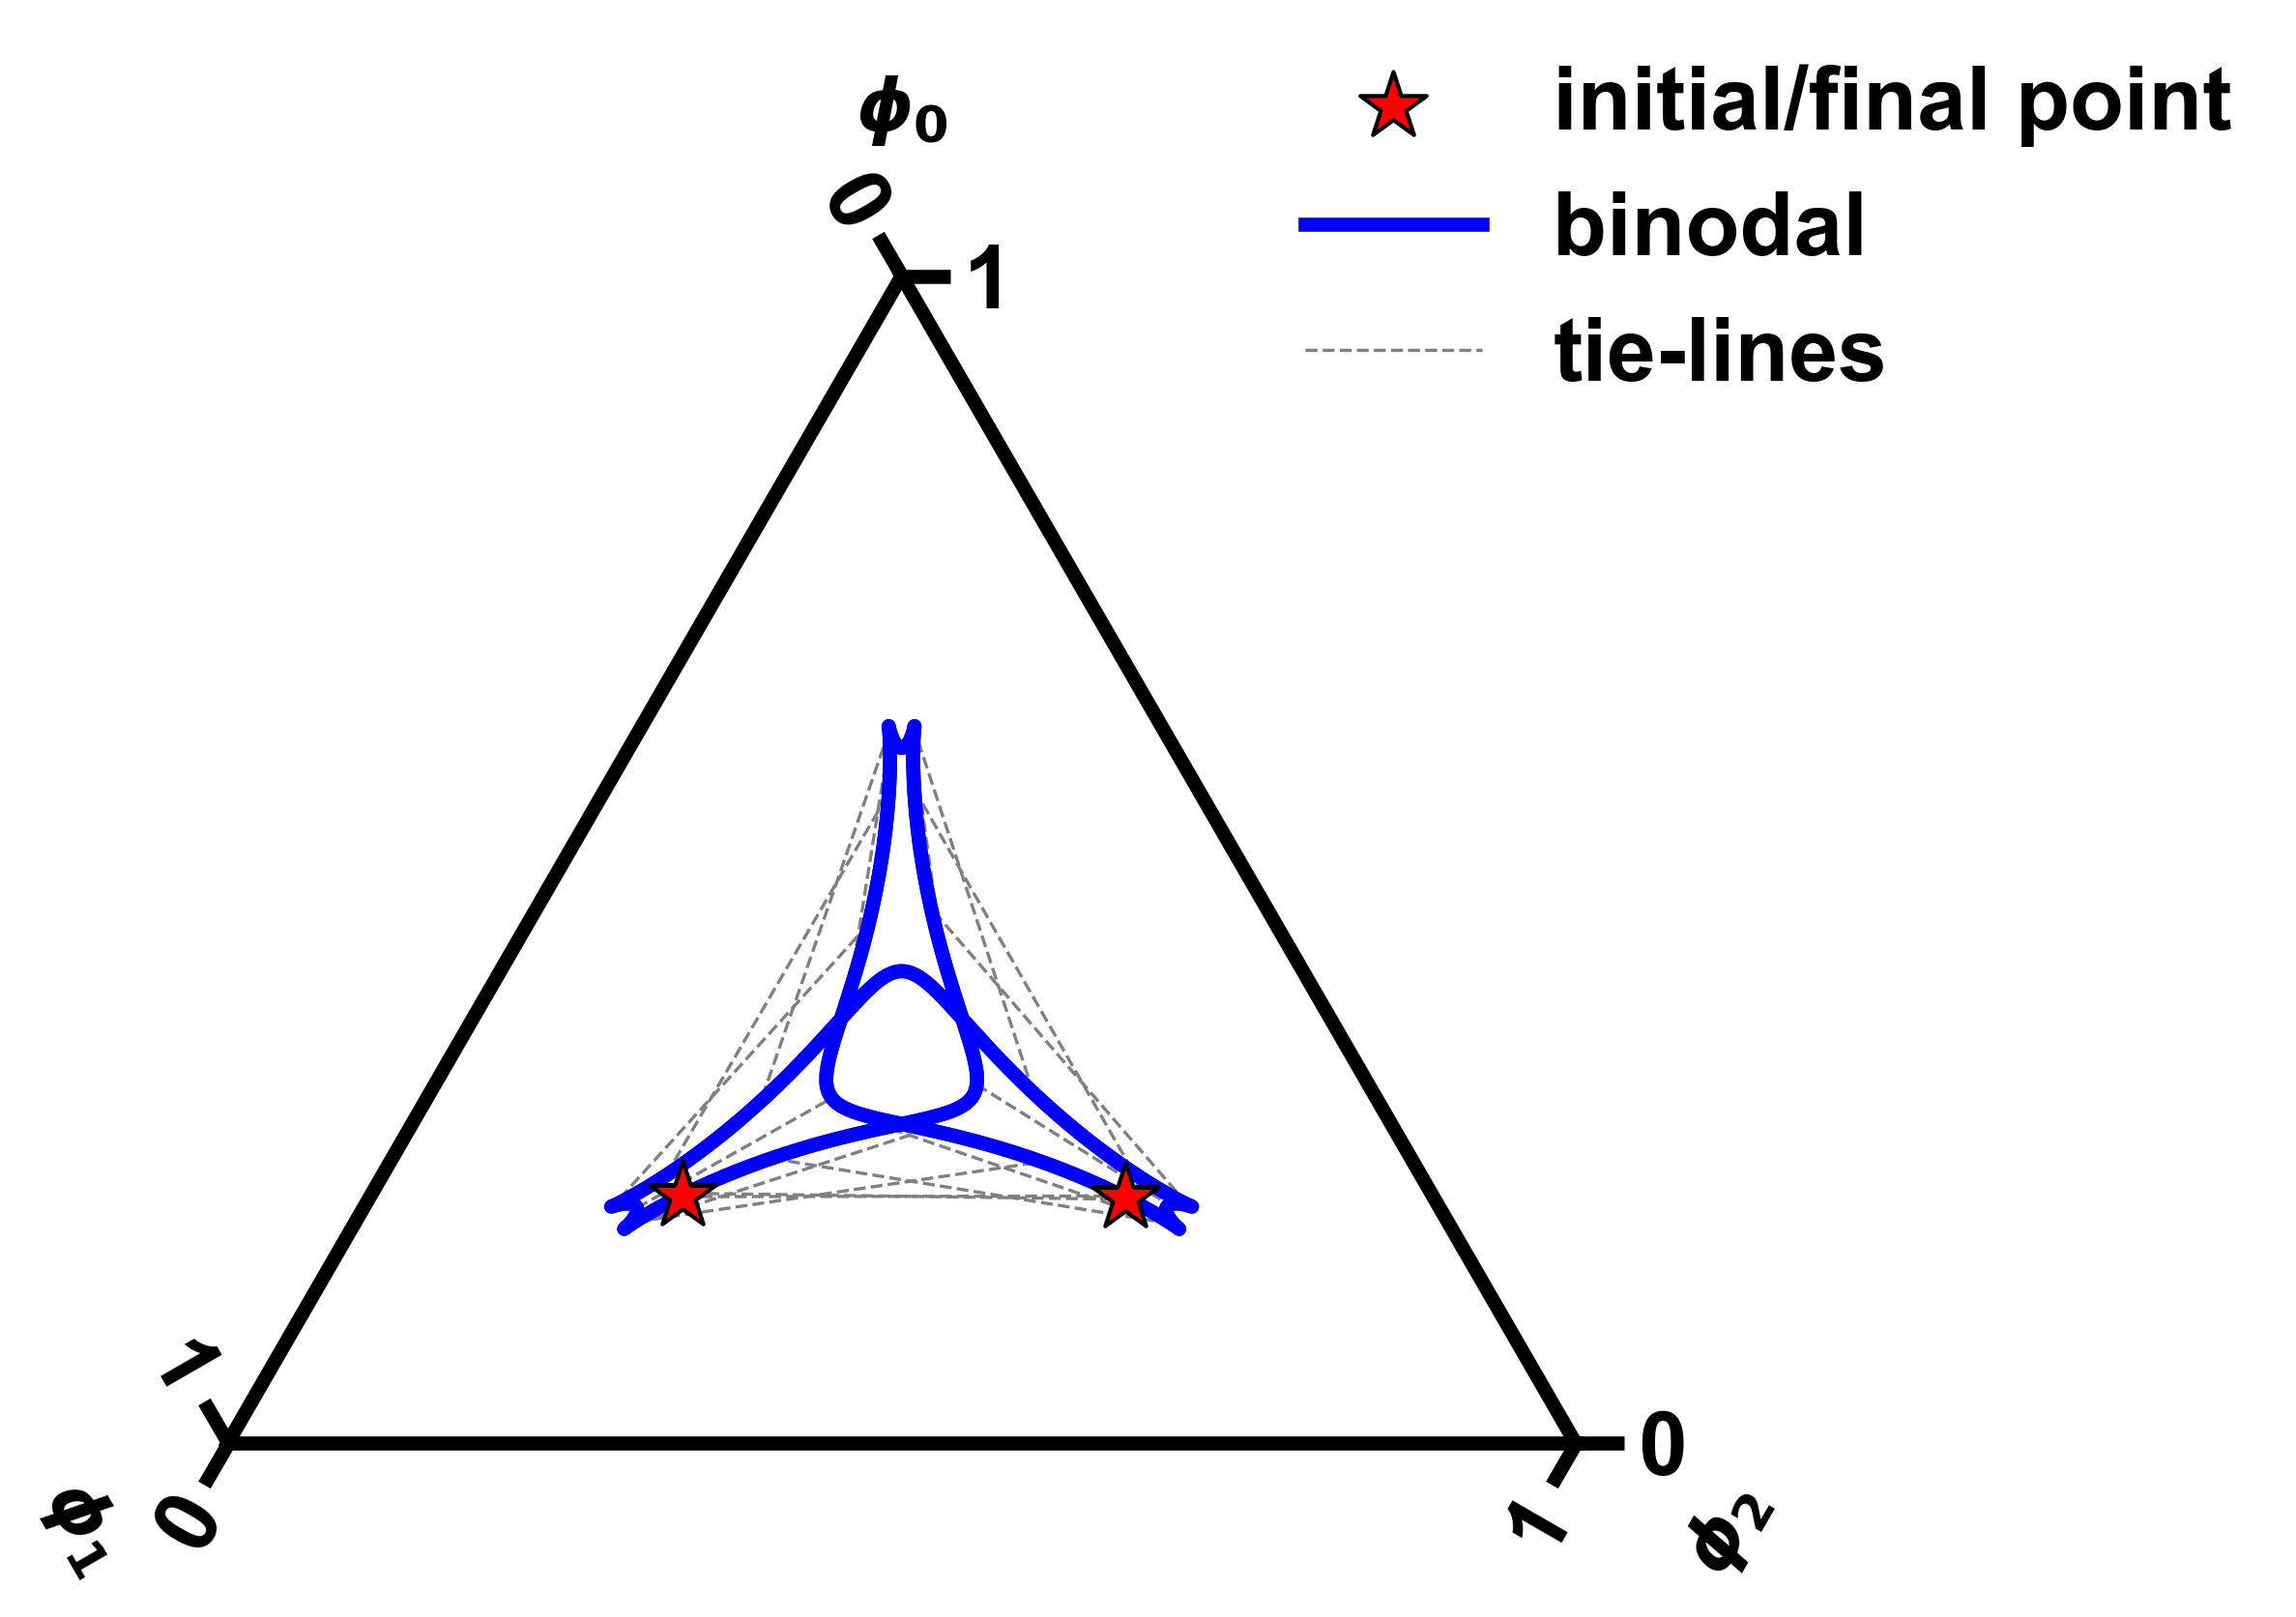
\includegraphics[width=0.8\textwidth]{figures/self_loop.png}
    \captionof{figure}{Example of a self-returning binodal section, which is a section of the binodal that loops back onto itself. The blue line shows the binodal and the gray dashed lines are the tie-lines. The red star indicates the point at which the binodal returns to its initial point.}
    \label{fig:self_loop}
\end{minipage}

\begin{table}
\centering
\caption{Numerical parameters of the continuation algorithm. Note that these values have been chosen to optimize accuracy rather than speed, since the algorithm is already quite fast compared to alternative methods.
For instance, decreasing the branching threshold of $10^{-3}$ suppresses false positive branching events, but increases the probability of false negatives, resulting in an incomplete reconstruction of the binodal.
}
\label{tab:numerical_parameters}
\begin{numvaluesbox}
\centering
\renewcommand{\arraystretch}{1.15}
\begin{tabular}{|p{0.28\textwidth}|p{0.49\textwidth}|p{0.13\textwidth}|}
\hline
\textbf{Parameter} & \textbf{Description} & \textbf{Default value} \\
\hline
Static tangential step size & Baseline step size used away from branching events. & \(10^{-2}\) \\
\hline
Adaptive tangential step size range & Step size used near branching events; scales with the second smallest singular value and is capped to avoid excessively small or large steps. & \([10^{-4},10^{-2}]\) \\
\hline
Adaptive-step threshold & Switch from static to adaptive tangential stepping when the second smallest singular value drops below this value. & \(10^{-1}\) \\
\hline
Branching threshold & Trigger branching events when the second smallest singular value falls below this value. & \(10^{-3}\) \\
\hline
Projection residual threshold & Stop the projection loop once \(\|\boldsymbol{E}(\boldsymbol{\phi})\|\) falls below this value. & \(10^{-10}\) \\
\hline
Critical-point termination threshold & Terminate tracing near a critical point when the Euclidean distance between the two coexisting phases falls below this value. & \(10^{-3}\) \\
\hline
Jacobian singular-value cutoff & Set singular values below this value to zero in order to stabilize the pseudoinverse near the critical point. & \(10^{-6}\) \\
\hline
Loop-back distance threshold & Terminate tracing if the current point returns sufficiently close to the initial point. & \(10^{-3}\) \\
\hline
Minimum steps before loop-back check & Delay the loop-back termination criterion to avoid spurious early termination. & \(10\) \\
\hline
\end{tabular}
\end{numvaluesbox}
\end{table}


\end{document}
